% Numerical experiments for sv_efficiency_proof.tex (included with % Numerical experiments for sv_efficiency_proof.tex (included with % Numerical experiments for sv_efficiency_proof.tex (included with % Numerical experiments for sv_efficiency_proof.tex (included with \input{numeric}).
% Data: examples/convection_diffusion/sv_numerics/run_numerics.py (output/*.json);
% tables and figures: make_figures.py -> tables/*.tex, figures/sv_*.{pdf,png}.
% All numbers quoted in the text below are read off those tables.

% ===========================================================================
\section{Numerical experiments}\label{sec:num}
% ===========================================================================

We test the estimator against the exact error. The questions are the ones raised by the theory:
\begin{enumerate}[label=(Q\arabic*)]
  \item Is the bound guaranteed, $E\le\eta_E$, in every run (Theorem~\ref{thm:rel})?
  \item Are the effectivity indices bounded independently of $\eps$, $\sigma$ and the stabilisation
  (Theorem~\ref{thm:eff}, Corollary~\ref{cor:two}), and do they stay bounded under refinement?
  \item Does the dependence on $c_b$ follow Corollaries~\ref{cor:two} and~\ref{cor:twoc}?
  \item Is the estimator locally efficient in the localisable measure (Theorem~\ref{thm:loc})?
  \item Do the indicators drive adaptive refinement to the optimal rate?
  \item Are the bounds valid at inexact iterates, and does the stopping criterion of
  Proposition~\ref{prop:stop} save iterations without spoiling the error?
  \item Does the variable-diffusion version keep its effectivity, with $\eta_\eps=O(h^2)$
  (Theorem~\ref{thm:vareps})?
\end{enumerate}

\subsection{Setup}

\paragraph{Discretisation.} Conforming $P_1$ elements on uniform meshes of the unit square
($n\times n$ squares, each cut into two triangles; $N=(n+1)^2$ vertices) or the unit cube ($n^3$
cubes, each cut into six tetrahedra), and on red--green refined meshes in the adaptive runs. The
stabilisations are the AFC scheme with the limiter of \cite{BJK17} (BJK), and the symmetrised
monotone upwind-type algebraic stabilisation of \cite{Kn23} (SMUAS). The nonlinear problem is solved
by the damped fixed-point iteration of \cite{AJ27} up to $\|r\|\le10^{-10}\sqrt N$, with at most
$2\cdot10^4$ iterations, unless stated otherwise.

\paragraph{Test problems} (all with $b$ constant, so $\sigma=c$, $c_b=1$ and $\kappa=3$, except in
Section~\ref{sec:num-cb}).
\begin{itemize}
  \item \emph{smooth}: $u=\prod_i\sin(\pi x_i)+x_1^2\prod_{i>1}x_i$, $b=(1,\tfrac12)$ or
  $(1,\tfrac12,\tfrac14)$, Dirichlet data on $\partial\Omega$; $f$ is computed from $u$. The solution
  has no layers, so its error is not dominated by layers, but for small $\eps$ the scheme is
  convection-dominated on every mesh used.
  \item \emph{layers}: $u=\prod_iw(x_i)$ with
  $w(s)=s-\bigl(e^{(s-1)/\eps}-e^{-1/\eps}\bigr)/\bigl(1-e^{-1/\eps}\bigr)$, $b=(1,\dots,1)$, homogeneous
  Dirichlet data; $u$ has exponential layers of width $\eps$ at the outflow boundary $x_i=1$.
  \item \emph{variable diffusion}: $u=\phi(x_1)\prod_{i>1}4x_i(1-x_i)$, either with
  $\eps(x)=\eps\,k^{x_1}$, $\phi(s)=4s(1-s)$ (\emph{smooth}), or with $\eps$ jumping from $\eps$ to $k\eps$
  at $x_1=\frac12$ and $\phi$ chosen such that the flux $\eps\phi'$ is continuous (\emph{jump}); $k$ is
  the contrast.
\end{itemize}

\paragraph{Error measures.} $\tnorm{e}$ is computed with a quadrature of degree~8. The dual norms
$\|B_A'(e,\cdot)\|_*$ and $\|\Stil\|_*$, and the local dual norms of $E_{\mathrm{loc}}$, are computed
from their Riesz representatives in the $P_2$ space on the same mesh (on each vertex patch for
$E_{\mathrm{loc}}$). These are \emph{lower} bounds of the true dual norms, so the reported effectivity
indices are slight overestimates; they become crude when the dual norm concentrates in layers that
the mesh does not resolve (see Section~\ref{sec:num-robust}). We report the effectivity indices
\[
  I=\frac{\eta}{\tnorm{e}},\qquad I_\oplus=\frac{\kappa\eta}{\tnorm{e}_\oplus},\qquad
  I_S=\frac{\eta_S}{\|\Stil\|_*},\qquad I_E=\frac{\eta_E}{E},
\]
of which $I_E$ is the one covered by Corollary~\ref{cor:two}; $I_\oplus\ge1$ and $I\ge1$ are guaranteed
too, but only $I_\oplus$ is expected to be robust.

\subsection{Solutions and indicators}

Figure~\ref{fig:snap} shows the discrete solution of the layers problem for $\eps=10^{-3}$ on the
$32\times32$ mesh, the cell indicators $\eta_K=\eta_{A,K}+\eta_{S,K}$, and the local energy errors
$\tnorm{e}_K$. The mesh does not resolve the layers ($h\approx4.4\cdot10^{-2}\gg\eps$); the AFC
solution is free of oscillations, and both the indicators and the error concentrate in the cells at
the outflow boundary, with a decay of several orders of magnitude into the interior. The indicator
is larger than $\tnorm{e}_K$ in the layer cells: it measures the residual in the dual norm, which
contains the convective part $\|B_A'(e,\cdot)\|_*$ of the error.

\begin{figure}[!htbp]
\centering
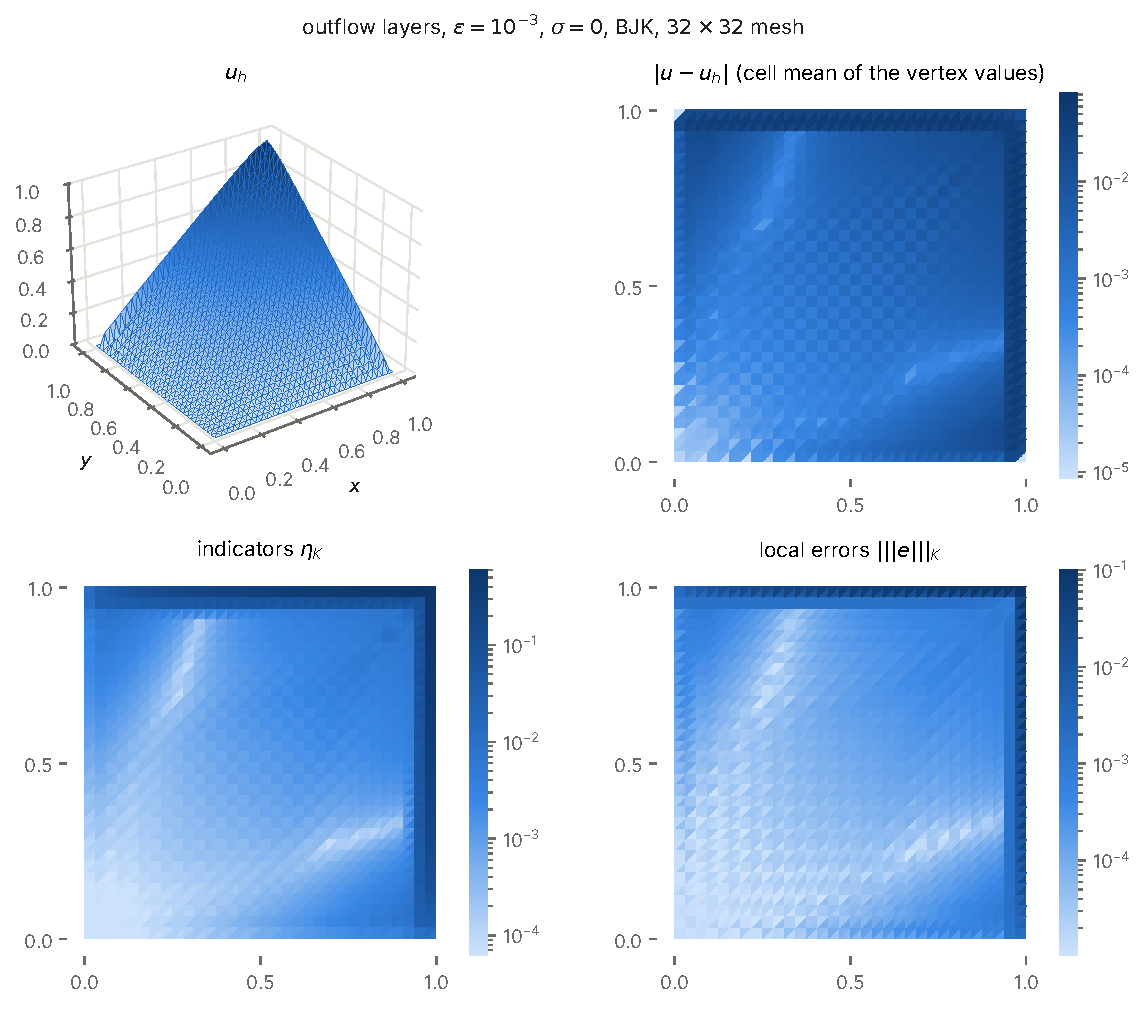
\includegraphics[width=\textwidth]{figures/sv_snap.pdf}
\caption{Layers problem, $\eps=10^{-3}$, $\sigma=0$, BJK, $n=32$: discrete solution $u_h$, indicators
$\eta_K$ and local errors $\tnorm{e}_K$ (logarithmic colour scale, common to both).}
\label{fig:snap}
\end{figure}

\subsection{Uniform refinement}\label{sec:num-conv}

Table~\ref{tab:conv} and Figure~\ref{fig:conv} report uniform refinement from $n=8$ to $n=128$.
\begin{itemize}
  \item \textbf{Smooth solution, $\eps=10^{-2}$.} $E$ and $\eta_E$ converge at the optimal rate $1$ in
  $h$ once the mesh resolves the solution; on the coarse meshes both decrease faster, because the
  stabilisation term $\|\Stil\|_*$ dominates $E$ there and decreases at a higher rate. The effectivity
  $I_E$ lies between $3.15$ and $3.29$ for $\sigma=0$ and $\sigma=1$ alike. The energy-norm index $I$
  tends to $1.1$: in the diffusion-dominated regime the energy norm and the dual norm of the
  residual coincide asymptotically.
  \item \textbf{Layers, $\eps=10^{-2}$.} The layers are resolved only from $n=64$ on, and the
  convergence of $E$ accelerates accordingly; $I_E$ stays between $2.77$ and $2.94$.
  \item \textbf{Layers, $\eps=10^{-4}$.} The meshes never resolve the layers. The energy error
  $\tnorm{e}$ \emph{increases} under refinement, because the error, concentrated in the outflow
  cells, sees an increasing part of the layer, while $E$ is dominated by the convective dual norm and
  decreases at the rate $0.45$--$0.53$; $\eta_E$ follows it with the rate $0.49$--$0.55$. The index $I_E$
  is $3.07$--$3.31$ on every mesh, whereas the energy-norm index $I$ falls from $833$ to $18.7$: the
  energy-norm bound is guaranteed but useless in this regime, which is why the error is measured in
  $E$.
\end{itemize}

\input{tables/conv}

\begin{figure}[!htbp]
\centering
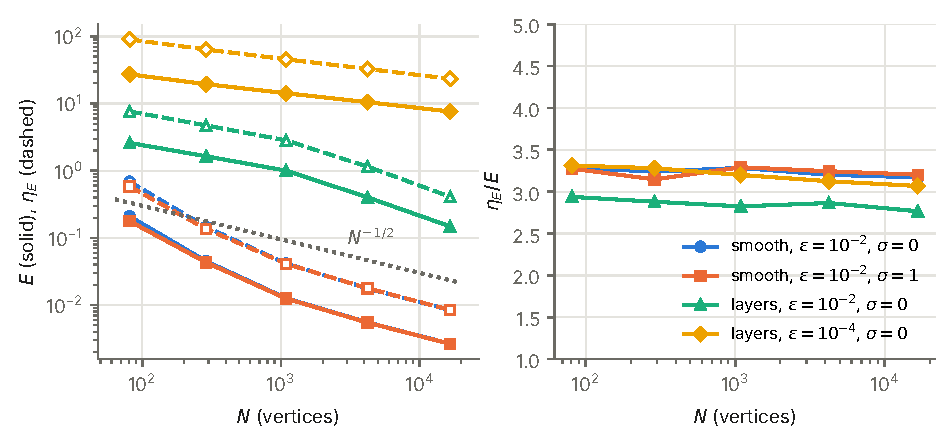
\includegraphics[width=\textwidth]{figures/sv_conv.pdf}
\caption{Uniform refinement in 2D, BJK. Left: $E$ (solid) and $\eta_E$ (dashed, open markers).
Right: effectivity index $I_E=\eta_E/E$.}
\label{fig:conv}
\end{figure}

\subsection{Robustness in \texorpdfstring{$\eps$}{eps}, \texorpdfstring{$\sigma$}{sigma} and the stabilisation}\label{sec:num-robust}

Table~\ref{tab:sweep} and Figure~\ref{fig:sweep} sweep $\eps$ from $10^{-1}$ to $10^{-8}$ on the fixed
mesh $n=32$, for $\sigma\in\{0,1\}$, both stabilisations and both problems.
\begin{itemize}
  \item \textbf{$\sigma=0$.} $I_E$ lies in $2.80$--$3.23$ for the layers problem and in $3.15$--$3.78$
  for the smooth problem, and becomes constant for $\eps\le10^{-5}$. $I_\oplus$ stays below $4.9$,
  and the stabilisation part is estimated sharply, $I_S=1.21$--$1.34$. BJK and SMUAS give the
  same indices $I_E$ and $I_\oplus$ to within $3\,\%$, as Remark~\ref{rem:robust} predicts: the limiter enters only
  through the functional, not the constants.
  \item \textbf{Energy norm.} The energy-norm index $I$ grows like $\eps^{-1}$ for $\sigma=0$, up to
  $2.5\cdot10^6$ at $\eps=10^{-8}$; the guaranteed energy-norm bound of \cite{ABR17} behaves in the
  same way. For $\sigma=1$, $I$ saturates at about $60$--$90$, the reaction giving $L^2$ control, while
  the ABR17 bound keeps growing ($1.3\cdot10^4$ at $\eps=10^{-8}$), because its reaction cut-off is not
  robust.
  \item \textbf{$\sigma=1$, small $\eps$.} Down to $\eps=10^{-6}$, $I_E$ stays in $2.7$--$3.2$ for the
  layers problem and in $3.2$--$4.9$ for the smooth one. For $\eps<10^{-6}$ it rises, to $5.5$ (layers)
  and $6.0$ (smooth) at $\eps=10^{-8}$. This increase comes from $I_S$ ($7.8$ and $10.4$ at
  $\eps=10^{-8}$), while $I_\oplus$ \emph{decreases}. This is consistent with a
  reference effect rather than with a loss of robustness: for $\sigma>0$, the Riesz representative of
  $\Stil$ has layers of width $(\eps/\sigma)^{1/2}=10^{-4}$, far below the mesh size $3\cdot10^{-2}$, so
  the same-mesh $P_2$ reference underestimates $\|\Stil\|_*$. Theorem~\ref{thm:eff} bounds $\eta_S$ by
  the true dual norm, independently of $\eps$. \adapt{The adaptive runs of Section~\ref{sec:num-unad} confirm this:
  once the mesh resolves the layers, $I_S$ falls to $1.5$--$1.6$ and $I_E$ to about $3$.} \asref{The
  asymptotic reference below makes this quantitative.}
\end{itemize}

\input{tables/sweep}

{\color{teal}
\paragraph{An asymptotically exact reference for $\|\Stil\|_*$.} For $\theta\ll1$ the dual norm of the
stabilisation functional can be evaluated without resolving its Riesz representative. With
$q=A\nabla u_h$ cellwise constant, $\Stil(v)=(q,\nabla v)=-\sum_F(\jump{q\cdot n},v)_F$ for $v\in H^1_D$, since
$\dv q=0$ in each cell. Away from the vertices, the Riesz representative is a sum of one-dimensional layers
$-\eps z''+\sigma z=\jump{q\cdot n}\,\delta_F$ across the faces, each of energy
$\jump{q\cdot n}^2/(2(\eps\sigma)^{1/2})$ per unit length. Hence
\begin{equation}\label{eq:Sasym}
  \|\Stil\|_*^2=\sum_{F\text{ interior}}\frac{\|\jump{q\cdot n}\|_F^2}{2(\eps\sigma)^{1/2}}\,\bigl(1+O(\theta)\bigr),
  \qquad \theta\to0,
\end{equation}
and the same sum over the faces interior to $\tilde\omega_K$ gives $\|\Stil\|_{*,\tilde\omega_K}^2$.
Table~\ref{tab:refref} and Figure~\ref{fig:refref} compare this value with $P_2$ references on the same mesh and on
$k$-times refined meshes ($k=2,4,8$), for the layers problem on the $16\times16$ mesh with $\sigma\in\{1,10^4\}$, using
the A+S estimator alone (without the direct variant of Remark~\ref{rem:direct}).
\begin{itemize}
  \item \textbf{The references.} At $\theta=0.11$ the asymptotic value agrees with the refined reference to $1\,\%$
  ($2.92$ against $2.95$). For smaller $\theta$ the $P_2$ references are far from converged: at $\theta=10^{-5}$ the
  same-mesh value underestimates $\|\Stil\|_*$ by a factor $85$, and even the $8$ times refined one by a factor $30$.
  \item \textbf{Theorem~\ref{thm:eff} for $\ell=-\Stil$.} Measured against \eqref{eq:Sasym}, the index
  $I_S=\eta_{-\Stil}/\|\Stil\|_*$ lies in $1.64$--$2.22$ for all $\theta\le10^{-2}$; the local ratio
  $\max_K\eta_{S,K}^2/\|\Stil\|_{*,\tilde\omega_K}^2$ lies in $0.58$--$1.56$. For this functional the theorem has no
  oscillation term, so this is a direct confirmation of robust global and local efficiency in the reaction regime.
  \item \textbf{The error measure.} With $\|\Stil\|_*$ from \eqref{eq:Sasym} and the other two parts of $E$ from the
  $8$ times refined mesh, $\eta_E/E$ stays in $8.3$--$10.2$ over three decades of $\theta$, whereas the same-mesh
  reference gives values up to $284$. The rises of $I_E$ in Table~\ref{tab:sweep} and in Section~\ref{sec:num-unad} at
  small $\theta$ are therefore an artifact of the reference, not a loss of robustness.
\end{itemize}
}

\input{tables/refref}

\begin{figure}[!htbp]
\centering
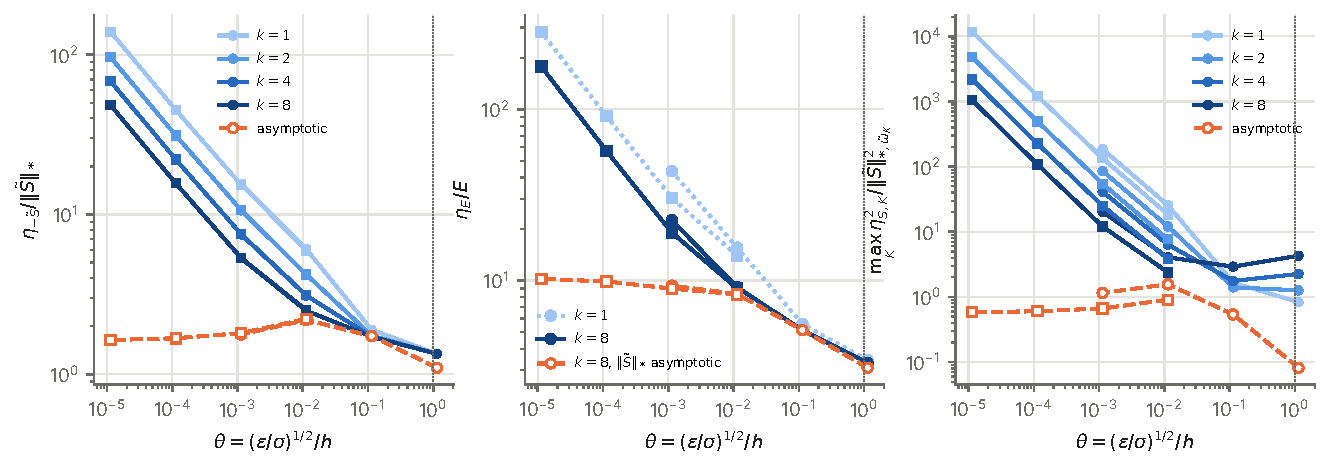
\includegraphics[width=\textwidth]{figures/sv_refref.pdf}
\caption{\asref{Reaction regime, layers problem, $n=16$, A+S estimator; circles $\sigma=1$, squares $\sigma=10^4$.
Left: $\eta_{-\Stil}/\|\Stil\|_*$ with $P_2$ references on $k$-times refined meshes and with the asymptotic value
\eqref{eq:Sasym}. Middle: $\eta_E/E$ with the same-mesh and the $8$ times refined references, and with
$\|\Stil\|_*$ from \eqref{eq:Sasym}. Right: the local ratio for $\ell=-\Stil$; the refined references are lower bounds
of the local dual norms, so these ratios are upper estimates; the asymptotic value is valid only for $\theta\ll1$.}}
\label{fig:refref}
\end{figure}

\begin{figure}[!htbp]
\centering
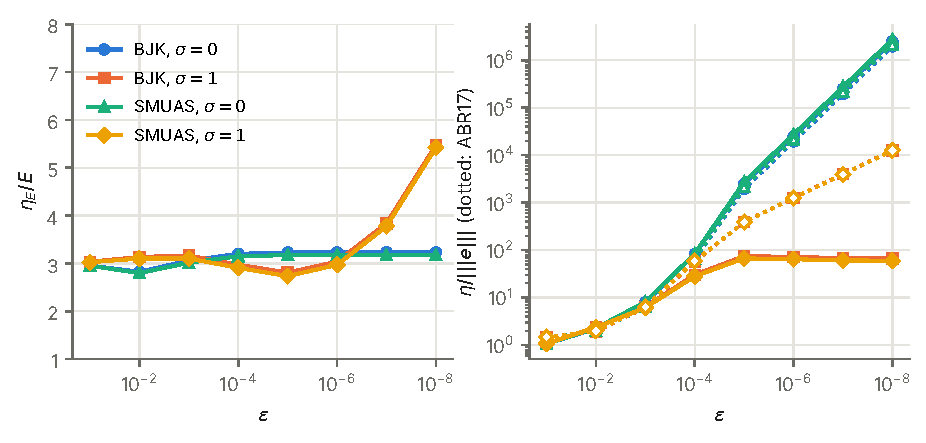
\includegraphics[width=\textwidth]{figures/sv_sweep.pdf}
\caption{Layers problem, $n=32$, as functions of $\eps$. Left: $I_E=\eta_E/E$. Right: the energy-norm
indices $\eta/\tnorm{e}$ (solid) and, dotted with open markers, that of the guaranteed bound of
\cite{ABR17}.}
\label{fig:sweep}
\end{figure}

\subsection{Variable reaction}\label{sec:num-cb}

With $c=1+(c_{\max}-1)xy$ and $\sigma=1$, the constant of (H3) is $\|c\|_\infty/\sigma=c_{\max}$, attained at
the vertex $(1,1)$. \refe{The computed $c_b$ is the sampled enclosure of Remark~\ref{rem:CF}, which is diagnostic: $c$ is not
affine on the cells, so the sampled maximum is enlarged by $\frac{h_K}2\max|\nabla c|$; here this gives} $c_b=1.12\,c_{\max}$, $1.06\,c_{\max}$
and $1.03\,c_{\max}$ for $n=8,16,32$, and $\kappa=2+c_b$ (Table~\ref{tab:cb}). The bound $E\le\eta_E$ holds in
all runs. The index of $\eta_{E,c}$ grows at most linearly, $\eta_{E,c}/E_c\le3\,c_b$ in all runs, as
Corollary~\ref{cor:twoc} predicts; it is often much smaller, down to $0.05\,c_b$, because the factor $M=c_b$ in front of $\tnorm{e}$ in $E_c$ also enlarges the
error measure. The index of $\eta_E$ grows faster, up to $5.2\,c_b$ at $c_b\approx10^3$, but stays far
below the worst case $(1+c_b)^2$ of Corollary~\ref{cor:two}. A variable reaction with a small lower
bound $\sigma$ is therefore the one situation in which the estimator loses its robustness, in
accordance with the theory; Section~\ref{sec:concl} discusses how to remove it.

\input{tables/cb}

\subsection{Local efficiency}\label{sec:num-loc}

Table~\ref{tab:loc} reports the localised measure for the layers problem on the $16\times16$ mesh. The
local ratio $\max_K\eta_K^2/E_{\mathrm{loc}}(\tilde\omega_K)^2$ is at most $0.51$ in all cases, and
independent of $\eps$ for $\eps\le10^{-4}$: the estimator is locally efficient, as stated in
Theorem~\ref{thm:loc}. The ratio $E_{\mathrm{loc}}/E$ lies between $0.48$ and $1.01$, so on these
problems the localised measure captures most of the global one, and the guaranteed bound
$E_{\mathrm{loc}}\le\sqrt{d+1}\,\eta_E$ of Theorem~\ref{thm:loc} overestimates $E_{\mathrm{loc}}$ by a
factor $5$--$12$. The largest value, $\eta_E/E_{\mathrm{loc}}=7.0$ for $\sigma=1$ and $\eps=10^{-8}$, is the
same reference effect as in Section~\ref{sec:num-robust}.

\input{tables/loc}

\subsection{Adaptive refinement}\label{sec:num-adapt}

Starting from the $8\times8$ mesh, we mark by the indicators $\eta_K=\eta_{A,K}+\eta_{S,K}$ with the
dual strategy of \cite{AJ27} (all cells with $\eta_K\ge\theta\max\eta$, $\theta=0.5$, reduced until at least
$5\,\%$ of the cells are marked) and refine by red--green refinement, until $N>3\cdot10^4$.
Table~\ref{tab:adapt} and Figures~\ref{fig:adapt} and~\ref{fig:adaptmesh} show the results for the layers
problem.
\begin{itemize}
  \item \textbf{Effectivity.} $I_E$ stays between $2.86$ and $3.55$ in every loop of all three runs, from
  $N=81$ to $N=45\,094$, while the local mesh size spans three orders of magnitude.
  \item \textbf{Where the mesh is refined.} The refinement concentrates in the outflow layers at $x=1$ and
  $y=1$ (Figure~\ref{fig:adaptmesh}); the smallest cells have $h_{\min}=3.5\cdot10^{-4}$ for $\eps=10^{-3}$,
  below $\eps$, so the layers are resolved, and $h_{\min}=1.7\cdot10^{-4}$ for $\eps=10^{-5}$, where they are not.
  \item \textbf{Convergence.} For $\eps=10^{-3}$, $E$ decreases at the rate $1.8$--$1.9$ with respect to
  $N^{-1/2}$ over the second half of the loops: this is the pre-asymptotic phase in which the layers become
  resolved, faster than the optimal rate $1$. For $\eps=10^{-5}$ the rate is $0.98$. On the finest uniform mesh
  ($N=16\,641$) the error $E$ is $18$, $4.4$ and $17$ times larger than the adaptive error at the same $N$.
  Under uniform refinement $E$ decreases at the rate $0.46$--$0.60$ for $\sigma=0$ and $0.04$--$0.51$ for
  $\sigma=1$, because the layers are never resolved; the index $I_E$ is $2.86$--$3.37$ there as well.
  \item \textbf{Energy norm.} Along the adaptive runs the energy-norm index $I$ falls from $29$ to $1.1$
  ($\eps=10^{-3}$) and from $8.4\cdot10^3$ to $6.2$ ($\eps=10^{-5}$): once the mesh resolves the layers, the
  energy error and the dual norm of the residual become comparable, while $I_E$ is insensitive to this.
\end{itemize}

\input{tables/adapt}

\begin{figure}[!htbp]
\centering
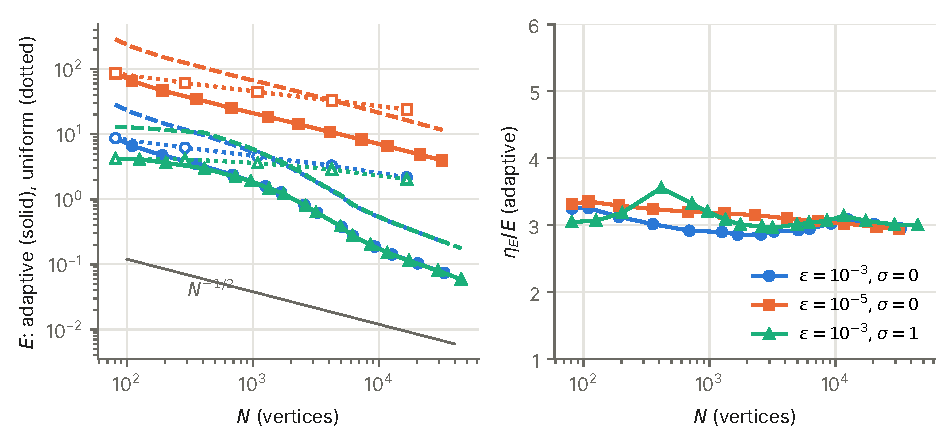
\includegraphics[width=\textwidth]{figures/sv_adapt.pdf}
\caption{Adaptive refinement, layers problem, BJK. Left: $E$ for adaptive (solid) and uniform (dotted, open
markers) refinement, and $\eta_E$ for the adaptive runs (dashed). Right: $I_E$ along the adaptive runs.}
\label{fig:adapt}
\end{figure}

\begin{figure}[!htbp]
\centering
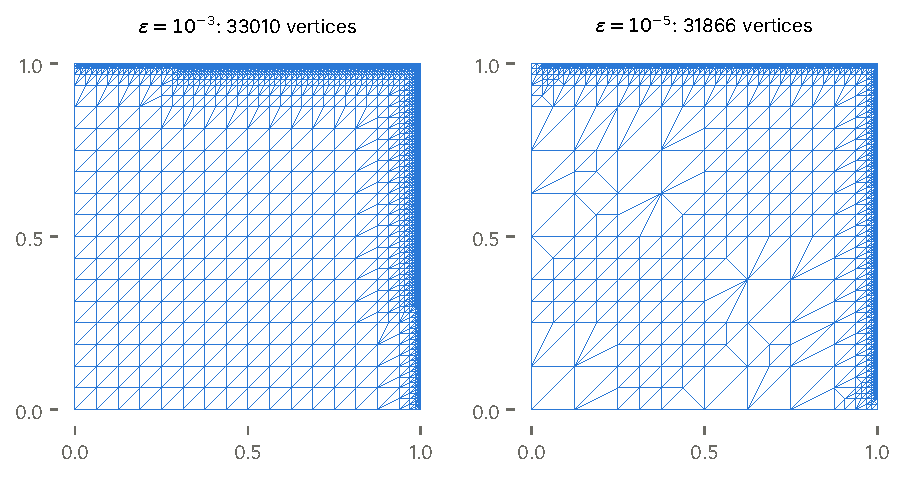
\includegraphics[width=\textwidth]{figures/sv_adapt_mesh.pdf}
\caption{Final adaptive meshes, layers problem, $\sigma=0$.}
\label{fig:adaptmesh}
\end{figure}

\subsection{\adapt{Uniform versus adaptive refinement}}\label{sec:num-unad}
{\color{magenta}

We repeat the uniform-mesh studies of Tables~\ref{tab:conv} and~\ref{tab:sweep} with adaptive refinement:
the same problems, the same marking as in Section~\ref{sec:num-adapt}, from the $8\times8$ mesh up to
$N\approx2\cdot10^4$ (Table~\ref{tab:conv}) and $N\approx10^4$ (Table~\ref{tab:sweep}). For the robustness
sweep we compare at equal cost: the adaptive loop whose $N$ is closest to $N=1089$, the size of the $32\times32$
mesh of Table~\ref{tab:sweep}.

\paragraph{Refinement studies (Figure~\ref{fig:aconv}).}
\begin{itemize}
  \item \textbf{Effectivity.} Along the adaptive runs $I_E$ lies in $2.83$--$4.18$ and tends to the same values
  as on uniform meshes, about $3.0$--$3.2$. The bound held in every loop.
  \item \textbf{Accuracy.} For the smooth solution, adaptive refinement gains nothing: at $N=16\,641$ the two
  errors agree to within $1\,\%$, and $E$ converges at the rate $1$ in both cases. For the layers problem the
  uniform error is $5.4$ ($\eps=10^{-2}$) and $5.9$ ($\eps=10^{-4}$) times the adaptive one at the same $N$.
  For $\eps=10^{-4}$, $E$ converges at the rate $0.47$ under uniform refinement and at $1.4$--$1.9$ in the last
  adaptive loops, in which the layers become resolved.
\end{itemize}

\begin{figure}[!htbp]
\centering
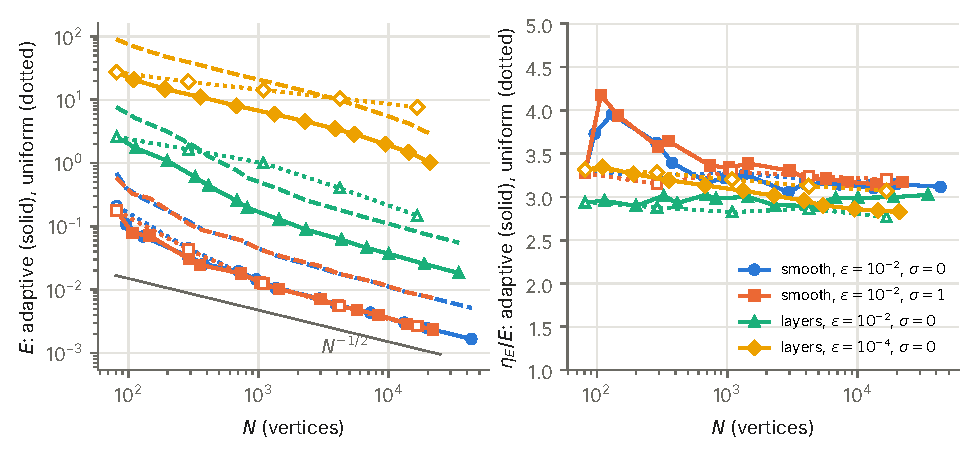
\includegraphics[width=\textwidth]{figures/sv_aconv.pdf}
\caption{\adapt{The cases of Table~\ref{tab:conv} under adaptive refinement. Left: $E$ for adaptive (solid) and uniform
(dotted, open markers) refinement, and $\eta_E$ for the adaptive runs (dashed). Right: $I_E$, adaptive (solid) and
uniform (dotted).}}
\label{fig:aconv}
\end{figure}

\paragraph{Robustness sweep (Figures~\ref{fig:abudget} and~\ref{fig:aloops}).}
\begin{itemize}
  \item \textbf{$\sigma=0$.} At equal cost, $I_E=2.89$--$3.22$ on the adaptive meshes against $2.80$--$3.23$ on the
  uniform mesh, for all $\eps$ and both stabilisations, and it stays in $2.82$--$3.35$ over all loops: the
  estimator is as robust on the meshes it generates as on the fixed mesh.
  \item \textbf{$\sigma=1$, small $\eps$.} The rise of $I_E$ to $5.4$--$5.5$ on the uniform mesh at
  $\eps\le10^{-7}$ (Section~\ref{sec:num-robust}) does not occur at equal cost on the adaptive meshes, where
  $I_E=2.75$--$3.16$. Figure~\ref{fig:aloops} shows why. The large values, up to $9.6$, appear only on the
  coarse initial mesh, and they come from the stabilisation part: $I_S=17.8$ at $N=81$ for $\eps=10^{-8}$. As the
  mesh resolves the layers, $I_S$ falls to $1.5$--$1.6$ and $I_E$ returns to about $3$. This confirms that the
  rise on the uniform mesh is a property of the under-resolved $P_2$ reference for $\|\Stil\|_*$, not of the
  estimator.
  \item \textbf{Smooth problem.} For $\eps\le10^{-3}$ the adaptive indices are higher than the uniform ones at
  equal cost: $I_E=4.0$--$5.3$ against $3.6$--$3.8$ for $\sigma=0$, and $4.5$--$6.0$ against $3.9$--$6.0$ for
  $\sigma=1$. Along the runs they reach $7.8$ after the first loop, and $10.9$ on the initial mesh. For $\sigma=1$
  and $\eps\le10^{-6}$ the fixed-point iteration reaches the iteration limit $2\cdot10^4$ on most meshes beyond
  $N\approx1100$, and the bound holds at these iterates.
  \item \textbf{Energy norm.} At $\sigma=0$ the energy-norm index still grows like $\eps^{-1}$ on the adaptive meshes,
  to $4\cdot10^5$ at $\eps=10^{-8}$ (uniform: $2.5\cdot10^6$); only the augmented measure is robust.
  \item \textbf{An open point.} For the layers problem with $\sigma=1$ and $\eps=10^{-6}$, $I_E$ rises again in the
  last loops, from $2.8$ to $4.3$, together with $I_\oplus$ (from $3.2$ to $6.6$). We have not identified the cause;
  it may be the convective part of the reference becoming resolved, and would need runs beyond $N=10^4$.
\end{itemize}

\begin{figure}[!htbp]
\centering
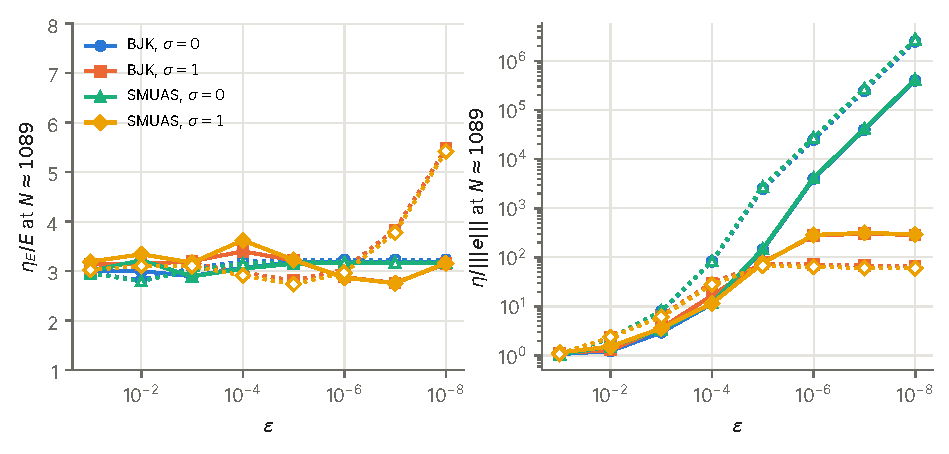
\includegraphics[width=\textwidth]{figures/sv_asweep_budget.pdf}
\caption{\adapt{The robustness sweep of Table~\ref{tab:sweep} at equal cost, layers problem: adaptive meshes with
$N\approx1089$ (solid) against the uniform $32\times32$ mesh (dotted, open markers). Left: $I_E$. Right: the
energy-norm index $\eta/\tnorm{e}$.}}
\label{fig:abudget}
\end{figure}

\begin{figure}[!htbp]
\centering
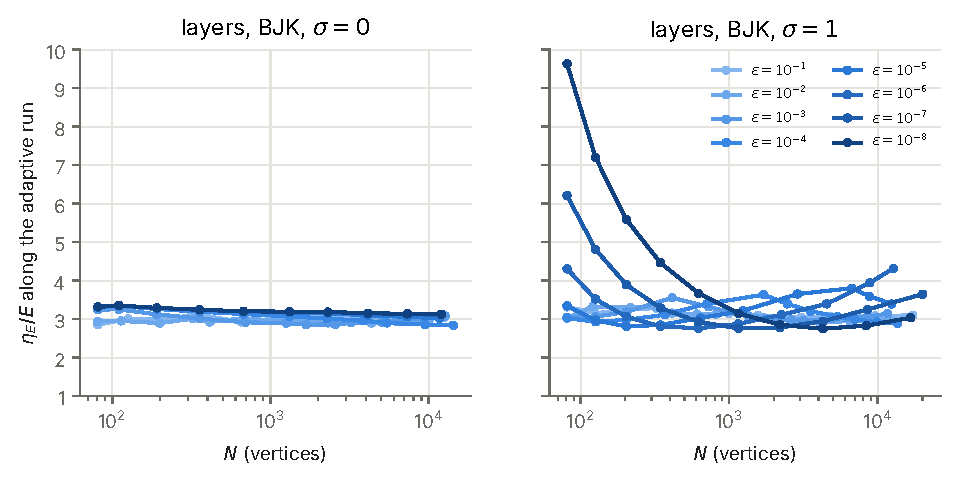
\includegraphics[width=\textwidth]{figures/sv_asweep_loops.pdf}
\caption{\adapt{$I_E$ along the adaptive runs of the robustness sweep, layers problem, BJK; one line per $\eps$, darker for
smaller $\eps$.}}
\label{fig:aloops}
\end{figure}

\paragraph{Which refinement to use.} For computing solutions, adaptive refinement is clearly preferable when the
solution has layers, by factors $4$--$18$ in $E$ at equal $N$, and it is what the estimator is designed for. For
testing the theory, the uniform meshes remain the primary evidence: a fixed coarse mesh keeps the layers
unresolved, which is the regime in which robustness can fail, isolates the dependence on $\eps$ and $\sigma$, and
is the only setting in which rates in $h$ are meaningful. The adaptive runs confirm that the effectivity stays at
about $3$ on the meshes the estimator generates itself.
}% end of the magenta block

\subsection{Inexact iterates and adaptive stopping}\label{sec:num-stop}

\paragraph{Iterates.} Table~\ref{tab:iter} and Figure~\ref{fig:iter} evaluate the estimator at the
fixed-point iterates $u^i$ on the $16\times16$ mesh. The index $I_E$ stays between $2.9$ and $5.3$ at
every iterate, including the first one, where the algebraic part $\eta_{\mathrm{alg}}$ is up to $71\,\%$
of $\eta_{\mathrm{disc}}$: this is part~2 of Proposition~\ref{prop:stop}, efficiency at every iterate
without any condition on the algebraic error. The ratio $\eta_{\mathrm{alg}}/\eta_{\mathrm{disc}}$
decreases monotonically for all problems except the smooth one with $\eps=10^{-6}$ and $\sigma=0$, for
which the fixed-point iteration does not converge in $2\cdot10^4$ iterations; there the ratio stalls
between $10^{-3}$ and $4\cdot10^{-3}$. In that case the error is smallest at $i\approx10$, $E(u^{10})=4.8$, and grows to
$8.4$ at $i=2\cdot10^4$: further iterations make the iterate worse in $E$, and the estimator, which is
efficient at every iterate, reflects this.

\input{tables/iter}

\begin{figure}[!htbp]
\centering
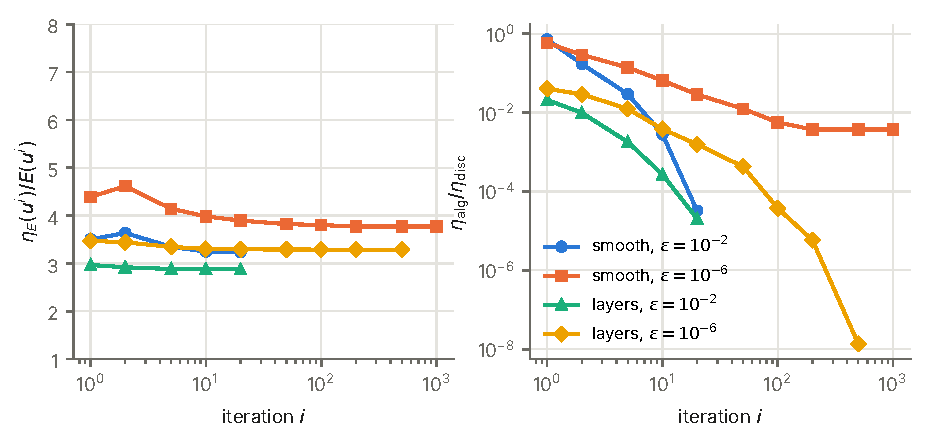
\includegraphics[width=\textwidth]{figures/sv_iter.pdf}
\caption{Fixed-point iterates, BJK, $\sigma=0$, $n=16$. Left: $I_E$ at the iterate $u^i$. Right: the
ratio $\eta_{\mathrm{alg}}/\eta_{\mathrm{disc}}$ (points with a ratio below $10^{-8}$ are omitted).}
\label{fig:iter}
\end{figure}

\paragraph{Adaptive stopping.} Table~\ref{tab:stop} runs five adaptive loops \refe{as in} Section~\ref{sec:num-adapt}
in which the fixed-point iteration is stopped either at the fixed tolerance $\|r\|\le10^{-10}\sqrt N$ or by
the criterion \eqref{eq:stop}, $\eta_{\mathrm{alg}}\le\gamma\eta_{\mathrm{disc}}$, with
$\eta_{\mathrm{disc}}=\eta_E-\eta_{\mathrm{alg}}$; each loop starts from the zero initial guess.
\begin{itemize}
  \item \textbf{Savings.} With $\gamma=0.1$, the total number of iterations drops from $227$ to $25$ (smooth,
  $\eps=10^{-2}$) and from $2323$ to $25$ (layers, $\eps=10^{-4}$), by factors $9$ and $93$; with $\gamma=0.01$
  the factors are $4.5$ and $46$.
  \item \textbf{Accuracy.} The final error $E$ changes by at most $6\,\%$ ($\gamma=0.1$, layers) and by at most
  $0.3\,\%$ for $\gamma\le0.01$. The index $I_E$ stays in $3.1$--$4.8$ in all runs, and in every stopped loop
  $\eta_{\mathrm{alg}}/\eta_{\mathrm{disc}}\le\gamma$, so $E\le(1+\gamma)\eta_{\mathrm{disc}}$
  (Proposition~\ref{prop:stop}, part~3).
  \item \textbf{Non-converging iteration.} For the smooth problem with $\eps=10^{-6}$ the fixed-point
  iteration does not reach the tolerance within $10^4$ iterations on any mesh, and $50\,000$ iterations give
  $E=3.22$. The criterion with $\gamma=0.1$ stops after $5$--$15$ iterations per loop, $50$ in total, with a
  \emph{smaller} error, $E=1.98$: as in Figure~\ref{fig:iter}, the early iterates are better than the late
  ones. For $\gamma=10^{-3}$ the criterion fires in only one of the five loops, since $\eta_{\mathrm{alg}}/\eta_{\mathrm{disc}}$ stalls
  at about $3\cdot10^{-3}$; this is a property of the iteration, not of the estimator.
\end{itemize}

\input{tables/stop}

\subsection{Variable diffusion}\label{sec:num-vareps}

Table~\ref{tab:vareps} reports the variable-diffusion problems on the meshes $n=8,16,32$. All bounds are
guaranteed. For the smooth coefficient, the oscillation $\eta_\eps$ converges at the rate $2.09$--$2.13$
in $h$, in accordance with Lemma~\ref{lem:V}(iii), and is at most $12\,\%$ of $\eta$ (at contrast $10^4$ on
the coarsest mesh). For the jump aligned with the mesh, $\Pi_1\eps=\eps$ and $\eta_\eps=0$. The
effectivity $I_E$ lies in $2.6$--$4.5$ for contrasts up to $10^4$, for $\eps=10^{-2}$ and $10^{-6}$ alike. For
the jump it does not grow with the contrast; for the smooth coefficient it grows mildly, from
$3.1$ at contrast $1$ to at most $4.3$ at contrast $10^4$ (on the coarsest mesh). This is the quasi-monotone case; the constants of
Theorem~\ref{thm:vareps} depend on the patch contrast, but for an aligned jump that contrast does not
show up in the indices. Checkerboard (non-quasi-monotone) coefficients are not tested; for them no
local estimator can be robust \cite{Li26}.

\input{tables/vareps}

\subsection{Three dimensions}\label{sec:num-3d}

Table~\ref{tab:d3} repeats the uniform-refinement study on the unit cube ($n=4,8,16$, up to $N=4913$
vertices and $24\,576$ tetrahedra).
\begin{itemize}
  \item \textbf{Layers.} $I_E=2.94$--$3.55$ for $\eps=10^{-2}$ and $10^{-6}$, as in two dimensions; $I_\oplus\le4.9$
  and $I_S=1.21$--$1.26$.
  \item \textbf{Smooth solution.} $I_E$ is higher than in two dimensions, $5.1$--$6.4$, but decreases under
  refinement for both values of $\eps$ ($5.97\to5.40$ and $6.39\to5.09$). These meshes are coarse: $E$ still
  converges at the pre-asymptotic rates $2.1$--$2.7$ in $h$, dominated by the stabilisation part
  $\|\Stil\|_*$, which is estimated sharply ($I_S=1.28$--$1.31$); the larger index comes from the convective
  dual norm on coarse tetrahedral meshes. For $\eps=10^{-6}$ on the finest mesh the fixed-point iteration does
  not converge within $2\cdot10^4$ iterations, and the bound still holds at the last iterate.
  \item \textbf{Energy norm.} As in two dimensions, $I$ is useless for $\sigma=0$ and small $\eps$
  ($1.0\cdot10^4$--$1.4\cdot10^5$ at $\eps=10^{-6}$, against $2.6$--$9.3$ at $\eps=10^{-2}$), while $I_E$ is not
  affected.
  \item \textbf{Cost.} The estimator takes about $8$\,s at $N=729$ and $220$--$240$\,s at $N=4913$ in our
  Python implementation; the cost is dominated by the vertex-patch problems in $\RTN$, whose size grows
  quickly with the number of tetrahedra per patch in three dimensions. The patch problems are independent and
  can be solved in parallel; the global $\RT_0$ defect problem takes a small fraction of the time.
\end{itemize}

\input{tables/d3}

\subsection{Summary}

The experiments answer the questions (Q1)--(Q7) as follows.
\begin{enumerate}[label=(Q\arabic*)]
  \item The bound $E\le\eta_E$ held in every run: two and three dimensions, both stabilisations,
  $\eps=10^{-1},\dots,10^{-8}$, $\sigma\in\{0,1\}$, variable reaction and diffusion, adaptive meshes and inexact
  iterates\refe{, and so did $I\ge1$, $I_\oplus\ge1$ and $I_S\ge1$. Since the references are lower bounds of the dual
  norms, this is a consistency check rather than a proof}.
  \item For constant coefficients, $I_E$ lies in $2.6$--$5.3$ in two dimensions, inexact iterates included,
  independently of $\eps$, $\sigma$, the stabilisation and the mesh; the only exception is a rise to $6.0$
  ($n=32$) and $7.1$ ($n=16$) at $\sigma=1$, $\eps\le10^{-7}$, \adapt{which the adaptive runs identify as an
  under-resolved reference for $\|\Stil\|_*$ (Section~\ref{sec:num-unad})}\asref{, as the asymptotically exact
  reference \eqref{eq:Sasym} confirms ($I_S=1.6$--$2.2$ and $\eta_E/E=8.3$--$10.2$ for $\theta$ down to $10^{-5}$)}; in three dimensions it is $2.9$--$6.4$ and
  decreases under refinement. The energy-norm index $I$, and the guaranteed bound of \cite{ABR17}, are not
  robust.
  \item The effectivity grows with $c_b$, at most linearly for $\eta_{E,c}$ and well below $c_b^2$ for $\eta_E$:
  a variable reaction with a small lower bound is the one case in which robustness is lost, as the theory
  predicts.
  \item The local ratio $\max_K\eta_K^2/E_{\mathrm{loc}}(\tilde\omega_K)^2$ is at most $0.51$.
  \item Adaptive refinement driven by $\eta_K$ resolves the layers and reduces $E$ by factors $4$--$18$
  against uniform refinement at equal $N$, with $I_E=2.9$--$3.6$ throughout. \adapt{Repeating the refinement and
  robustness studies adaptively gives the same effectivity, about $3$, as on uniform meshes.}
  \item The estimator is efficient at every iterate, and the stopping criterion saves up to $99\,\%$ of the
  iterations at a change of the error of at most $6\,\%$ ($\gamma=0.1$) or $0.3\,\%$ ($\gamma\le0.01$).
  \item For variable diffusion, $\eta_\eps$ converges at rate $2$ and $I_E$ stays in $2.6$--$4.5$ up to contrast
  $10^4$.
\end{enumerate}

\paragraph{Reproducibility.} All results are produced by the scripts \texttt{run\_numerics.py} and
\texttt{make\_figures.py} in the directory
\path{examples/convection_diffusion/sv_numerics} of \texttt{galerkit}. The first runs the experiments (about
$35$ minutes on four cores, the three-dimensional runs sequentially because of their memory use); the
second writes the tables, the figures and, for every stored solution, a VTK file
(\texttt{.vtu}) with $u_h$, $u$, $u-u_h$, $\eps$, $\eta_K$, $\tnorm{e}_K$ and the local effectivity
$\eta_K/\tnorm{e}_K$. \adapt{The figures of Section~\ref{sec:num-unad} are produced by
\texttt{make\_adaptive\_figures.py} in the same directory.}

).
% Data: examples/convection_diffusion/sv_numerics/run_numerics.py (output/*.json);
% tables and figures: make_figures.py -> tables/*.tex, figures/sv_*.{pdf,png}.
% All numbers quoted in the text below are read off those tables.

% ===========================================================================
\section{Numerical experiments}\label{sec:num}
% ===========================================================================

We test the estimator against the exact error. The questions are the ones raised by the theory:
\begin{enumerate}[label=(Q\arabic*)]
  \item Is the bound guaranteed, $E\le\eta_E$, in every run (Theorem~\ref{thm:rel})?
  \item Are the effectivity indices bounded independently of $\eps$, $\sigma$ and the stabilisation
  (Theorem~\ref{thm:eff}, Corollary~\ref{cor:two}), and do they stay bounded under refinement?
  \item Does the dependence on $c_b$ follow Corollaries~\ref{cor:two} and~\ref{cor:twoc}?
  \item Is the estimator locally efficient in the localisable measure (Theorem~\ref{thm:loc})?
  \item Do the indicators drive adaptive refinement to the optimal rate?
  \item Are the bounds valid at inexact iterates, and does the stopping criterion of
  Proposition~\ref{prop:stop} save iterations without spoiling the error?
  \item Does the variable-diffusion version keep its effectivity, with $\eta_\eps=O(h^2)$
  (Theorem~\ref{thm:vareps})?
\end{enumerate}

\subsection{Setup}

\paragraph{Discretisation.} Conforming $P_1$ elements on uniform meshes of the unit square
($n\times n$ squares, each cut into two triangles; $N=(n+1)^2$ vertices) or the unit cube ($n^3$
cubes, each cut into six tetrahedra), and on red--green refined meshes in the adaptive runs. The
stabilisations are the AFC scheme with the limiter of \cite{BJK17} (BJK), and the symmetrised
monotone upwind-type algebraic stabilisation of \cite{Kn23} (SMUAS). The nonlinear problem is solved
by the damped fixed-point iteration of \cite{AJ27} up to $\|r\|\le10^{-10}\sqrt N$, with at most
$2\cdot10^4$ iterations, unless stated otherwise.

\paragraph{Test problems} (all with $b$ constant, so $\sigma=c$, $c_b=1$ and $\kappa=3$, except in
Section~\ref{sec:num-cb}).
\begin{itemize}
  \item \emph{smooth}: $u=\prod_i\sin(\pi x_i)+x_1^2\prod_{i>1}x_i$, $b=(1,\tfrac12)$ or
  $(1,\tfrac12,\tfrac14)$, Dirichlet data on $\partial\Omega$; $f$ is computed from $u$. The solution
  has no layers, so its error is not dominated by layers, but for small $\eps$ the scheme is
  convection-dominated on every mesh used.
  \item \emph{layers}: $u=\prod_iw(x_i)$ with
  $w(s)=s-\bigl(e^{(s-1)/\eps}-e^{-1/\eps}\bigr)/\bigl(1-e^{-1/\eps}\bigr)$, $b=(1,\dots,1)$, homogeneous
  Dirichlet data; $u$ has exponential layers of width $\eps$ at the outflow boundary $x_i=1$.
  \item \emph{variable diffusion}: $u=\phi(x_1)\prod_{i>1}4x_i(1-x_i)$, either with
  $\eps(x)=\eps\,k^{x_1}$, $\phi(s)=4s(1-s)$ (\emph{smooth}), or with $\eps$ jumping from $\eps$ to $k\eps$
  at $x_1=\frac12$ and $\phi$ chosen such that the flux $\eps\phi'$ is continuous (\emph{jump}); $k$ is
  the contrast.
\end{itemize}

\paragraph{Error measures.} $\tnorm{e}$ is computed with a quadrature of degree~8. The dual norms
$\|B_A'(e,\cdot)\|_*$ and $\|\Stil\|_*$, and the local dual norms of $E_{\mathrm{loc}}$, are computed
from their Riesz representatives in the $P_2$ space on the same mesh (on each vertex patch for
$E_{\mathrm{loc}}$). These are \emph{lower} bounds of the true dual norms, so the reported effectivity
indices are slight overestimates; they become crude when the dual norm concentrates in layers that
the mesh does not resolve (see Section~\ref{sec:num-robust}). We report the effectivity indices
\[
  I=\frac{\eta}{\tnorm{e}},\qquad I_\oplus=\frac{\kappa\eta}{\tnorm{e}_\oplus},\qquad
  I_S=\frac{\eta_S}{\|\Stil\|_*},\qquad I_E=\frac{\eta_E}{E},
\]
of which $I_E$ is the one covered by Corollary~\ref{cor:two}; $I_\oplus\ge1$ and $I\ge1$ are guaranteed
too, but only $I_\oplus$ is expected to be robust.

\subsection{Solutions and indicators}

Figure~\ref{fig:snap} shows the discrete solution of the layers problem for $\eps=10^{-3}$ on the
$32\times32$ mesh, the cell indicators $\eta_K=\eta_{A,K}+\eta_{S,K}$, and the local energy errors
$\tnorm{e}_K$. The mesh does not resolve the layers ($h\approx4.4\cdot10^{-2}\gg\eps$); the AFC
solution is free of oscillations, and both the indicators and the error concentrate in the cells at
the outflow boundary, with a decay of several orders of magnitude into the interior. The indicator
is larger than $\tnorm{e}_K$ in the layer cells: it measures the residual in the dual norm, which
contains the convective part $\|B_A'(e,\cdot)\|_*$ of the error.

\begin{figure}[!htbp]
\centering
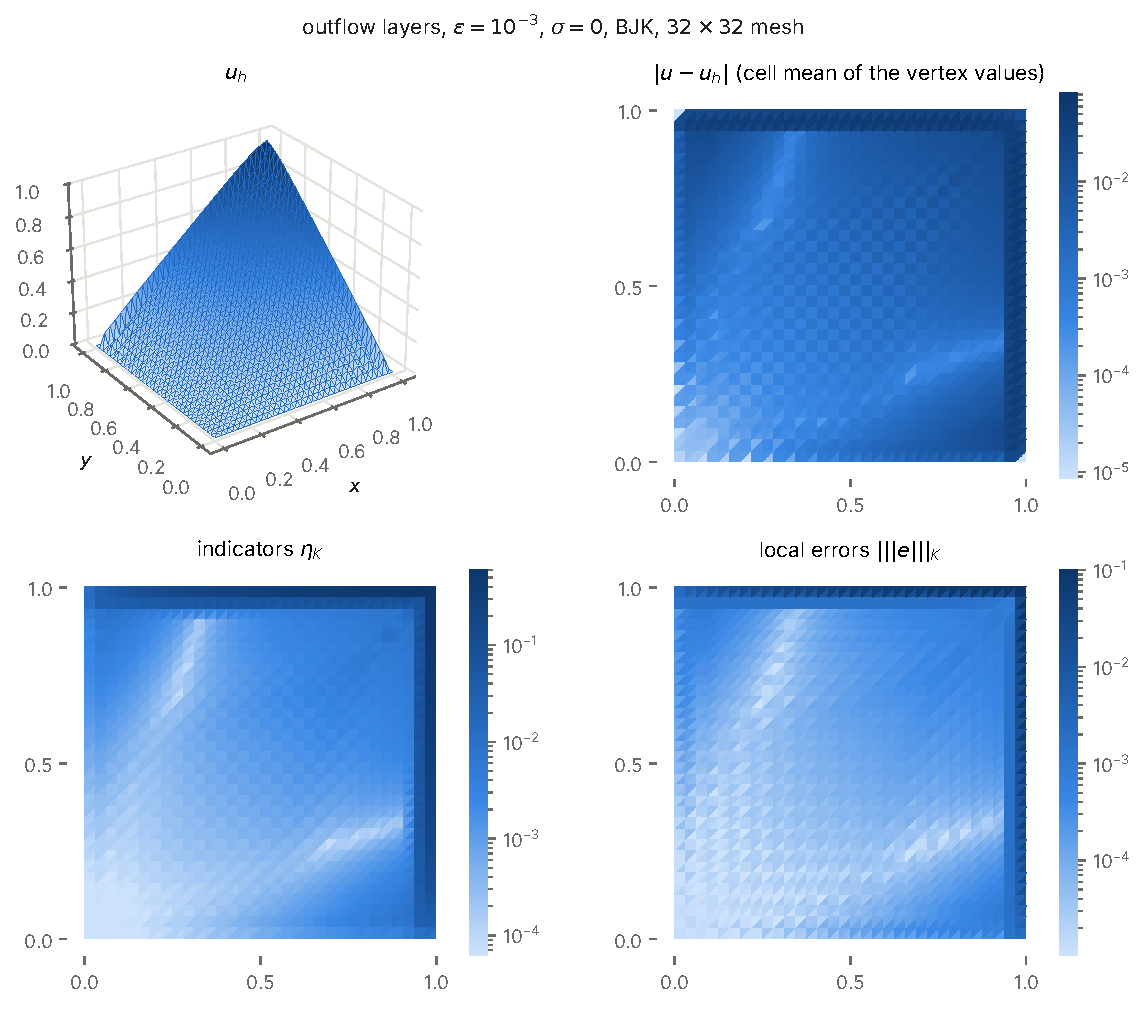
\includegraphics[width=\textwidth]{figures/sv_snap.pdf}
\caption{Layers problem, $\eps=10^{-3}$, $\sigma=0$, BJK, $n=32$: discrete solution $u_h$, indicators
$\eta_K$ and local errors $\tnorm{e}_K$ (logarithmic colour scale, common to both).}
\label{fig:snap}
\end{figure}

\subsection{Uniform refinement}\label{sec:num-conv}

Table~\ref{tab:conv} and Figure~\ref{fig:conv} report uniform refinement from $n=8$ to $n=128$.
\begin{itemize}
  \item \textbf{Smooth solution, $\eps=10^{-2}$.} $E$ and $\eta_E$ converge at the optimal rate $1$ in
  $h$ once the mesh resolves the solution; on the coarse meshes both decrease faster, because the
  stabilisation term $\|\Stil\|_*$ dominates $E$ there and decreases at a higher rate. The effectivity
  $I_E$ lies between $3.15$ and $3.29$ for $\sigma=0$ and $\sigma=1$ alike. The energy-norm index $I$
  tends to $1.1$: in the diffusion-dominated regime the energy norm and the dual norm of the
  residual coincide asymptotically.
  \item \textbf{Layers, $\eps=10^{-2}$.} The layers are resolved only from $n=64$ on, and the
  convergence of $E$ accelerates accordingly; $I_E$ stays between $2.77$ and $2.94$.
  \item \textbf{Layers, $\eps=10^{-4}$.} The meshes never resolve the layers. The energy error
  $\tnorm{e}$ \emph{increases} under refinement, because the error, concentrated in the outflow
  cells, sees an increasing part of the layer, while $E$ is dominated by the convective dual norm and
  decreases at the rate $0.45$--$0.53$; $\eta_E$ follows it with the rate $0.49$--$0.55$. The index $I_E$
  is $3.07$--$3.31$ on every mesh, whereas the energy-norm index $I$ falls from $833$ to $18.7$: the
  energy-norm bound is guaranteed but useless in this regime, which is why the error is measured in
  $E$.
\end{itemize}

% generated by examples/convection_diffusion/sv_numerics/make_figures.py; do not edit
\begin{table}[!htbp]
\centering
\small
\setlength{\tabcolsep}{4pt}
\caption{Uniform refinement in 2D, BJK. Rates with respect to $N^{-1/2}\sim h$; the expected rate is $1$ once the mesh resolves the solution. Effectivity indices $I=\eta/\tnorm{e}$, $I_\oplus=\kappa\eta/\tnorm{e}_\oplus$, $I_E=\eta_E/E$; the last column is the number of fixed-point iterations.}\label{tab:conv}
\begin{tabular}{rlllrlrrrr}
\toprule
$N$ & $\tnorm{e}$ & $E$ & rate & $\eta_E$ & rate & $I$ & $I_\oplus$ & $I_E$ & it.\\
\midrule
\multicolumn{10}{l}{\emph{smooth, $\eps=10^{-2}$, $\sigma=0$}}\\
81 & $4.88\cdot10^{-2}$ & $0.209$ &  & $0.687$ &  & 4.12 & 4.22 & 3.29 & 59\\
289 & $2.15\cdot10^{-2}$ & $4.48\cdot10^{-2}$ & 2.42 & $0.145$ & 2.45 & 2.05 & 3.86 & 3.24 & 39\\
1089 & $1.04\cdot10^{-2}$ & $1.26\cdot10^{-2}$ & 1.91 & $4.15\cdot10^{-2}$ & 1.89 & 1.31 & 3.46 & 3.28 & 18\\
4225 & $5.16\cdot10^{-3}$ & $5.51\cdot10^{-3}$ & 1.23 & $1.76\cdot10^{-2}$ & 1.26 & 1.14 & 3.24 & 3.20 & 9\\
16641 & $2.58\cdot10^{-3}$ & $2.65\cdot10^{-3}$ & 1.07 & $8.40\cdot10^{-3}$ & 1.08 & 1.09 & 3.18 & 3.17 & 6\\
\multicolumn{10}{l}{\emph{smooth, $\eps=10^{-2}$, $\sigma=1$}}\\
81 & $5.01\cdot10^{-2}$ & $0.178$ &  & $0.582$ &  & 3.34 & 4.04 & 3.27 & 56\\
289 & $2.16\cdot10^{-2}$ & $4.31\cdot10^{-2}$ & 2.23 & $0.136$ & 2.29 & 1.89 & 3.69 & 3.15 & 37\\
1089 & $1.04\cdot10^{-2}$ & $1.25\cdot10^{-2}$ & 1.87 & $4.12\cdot10^{-2}$ & 1.80 & 1.29 & 3.46 & 3.29 & 18\\
4225 & $5.16\cdot10^{-3}$ & $5.47\cdot10^{-3}$ & 1.22 & $1.77\cdot10^{-2}$ & 1.24 & 1.15 & 3.29 & 3.24 & 9\\
16641 & $2.58\cdot10^{-3}$ & $2.64\cdot10^{-3}$ & 1.06 & $8.45\cdot10^{-3}$ & 1.08 & 1.10 & 3.22 & 3.20 & 6\\
\multicolumn{10}{l}{\emph{layers, $\eps=10^{-2}$, $\sigma=0$}}\\
81 & $0.522$ & $2.6$ &  & $7.62$ &  & 4.19 & 3.78 & 2.94 & 67\\
289 & $0.471$ & $1.64$ & 0.72 & $4.72$ & 0.75 & 2.88 & 3.64 & 2.88 & 47\\
1089 & $0.366$ & $1$ & 0.74 & $2.83$ & 0.77 & 2.21 & 3.56 & 2.82 & 63\\
4225 & $0.231$ & $0.401$ & 1.35 & $1.15$ & 1.33 & 1.52 & 3.26 & 2.86 & 28\\
16641 & $0.127$ & $0.148$ & 1.46 & $0.409$ & 1.51 & 1.07 & 2.77 & 2.77 & 9\\
\multicolumn{10}{l}{\emph{layers, $\eps=10^{-4}$, $\sigma=0$}}\\
81 & $3.07\cdot10^{-2}$ & $2.72\cdot10^{1}$ &  & $9.02\cdot10^{1}$ &  & 833.01 & 4.76 & 3.31 & 405\\
289 & $6.15\cdot10^{-2}$ & $1.94\cdot10^{1}$ & 0.53 & $6.37\cdot10^{1}$ & 0.55 & 290.45 & 4.81 & 3.28 & 709\\
1089 & $0.154$ & $1.42\cdot10^{1}$ & 0.47 & $4.56\cdot10^{1}$ & 0.51 & 82.17 & 4.75 & 3.20 & 700\\
4225 & $0.242$ & $1.05\cdot10^{1}$ & 0.45 & $3.27\cdot10^{1}$ & 0.49 & 37.26 & 4.65 & 3.12 & 626\\
16641 & $0.342$ & $7.6$ & 0.47 & $2.33\cdot10^{1}$ & 0.49 & 18.72 & 4.54 & 3.07 & 566\\
\bottomrule
\end{tabular}
\end{table}


\begin{figure}[!htbp]
\centering
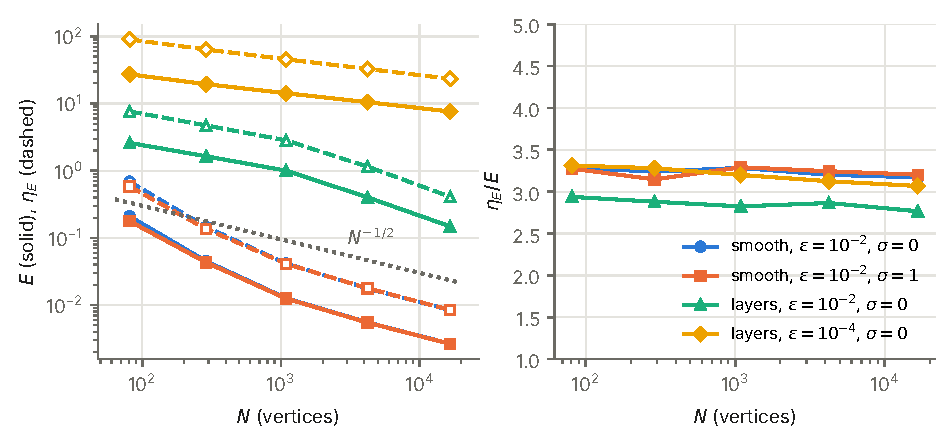
\includegraphics[width=\textwidth]{figures/sv_conv.pdf}
\caption{Uniform refinement in 2D, BJK. Left: $E$ (solid) and $\eta_E$ (dashed, open markers).
Right: effectivity index $I_E=\eta_E/E$.}
\label{fig:conv}
\end{figure}

\subsection{Robustness in \texorpdfstring{$\eps$}{eps}, \texorpdfstring{$\sigma$}{sigma} and the stabilisation}\label{sec:num-robust}

Table~\ref{tab:sweep} and Figure~\ref{fig:sweep} sweep $\eps$ from $10^{-1}$ to $10^{-8}$ on the fixed
mesh $n=32$, for $\sigma\in\{0,1\}$, both stabilisations and both problems.
\begin{itemize}
  \item \textbf{$\sigma=0$.} $I_E$ lies in $2.80$--$3.23$ for the layers problem and in $3.15$--$3.78$
  for the smooth problem, and becomes constant for $\eps\le10^{-5}$. $I_\oplus$ stays below $4.9$,
  and the stabilisation part is estimated sharply, $I_S=1.21$--$1.34$. BJK and SMUAS give the
  same indices $I_E$ and $I_\oplus$ to within $3\,\%$, as Remark~\ref{rem:robust} predicts: the limiter enters only
  through the functional, not the constants.
  \item \textbf{Energy norm.} The energy-norm index $I$ grows like $\eps^{-1}$ for $\sigma=0$, up to
  $2.5\cdot10^6$ at $\eps=10^{-8}$; the guaranteed energy-norm bound of \cite{ABR17} behaves in the
  same way. For $\sigma=1$, $I$ saturates at about $60$--$90$, the reaction giving $L^2$ control, while
  the ABR17 bound keeps growing ($1.3\cdot10^4$ at $\eps=10^{-8}$), because its reaction cut-off is not
  robust.
  \item \textbf{$\sigma=1$, small $\eps$.} Down to $\eps=10^{-6}$, $I_E$ stays in $2.7$--$3.2$ for the
  layers problem and in $3.2$--$4.9$ for the smooth one. For $\eps<10^{-6}$ it rises, to $5.5$ (layers)
  and $6.0$ (smooth) at $\eps=10^{-8}$. This increase comes from $I_S$ ($7.8$ and $10.4$ at
  $\eps=10^{-8}$), while $I_\oplus$ \emph{decreases}. This is consistent with a
  reference effect rather than with a loss of robustness: for $\sigma>0$, the Riesz representative of
  $\Stil$ has layers of width $(\eps/\sigma)^{1/2}=10^{-4}$, far below the mesh size $3\cdot10^{-2}$, so
  the same-mesh $P_2$ reference underestimates $\|\Stil\|_*$. Theorem~\ref{thm:eff} bounds $\eta_S$ by
  the true dual norm, independently of $\eps$. \adapt{The adaptive runs of Section~\ref{sec:num-unad} confirm this:
  once the mesh resolves the layers, $I_S$ falls to $1.5$--$1.6$ and $I_E$ to about $3$.} \asref{The
  asymptotic reference below makes this quantitative.}
\end{itemize}

% generated by examples/convection_diffusion/sv_numerics/make_figures.py; do not edit
\begin{table}[!htbp]
\centering
\footnotesize
\setlength{\tabcolsep}{4pt}
\caption{Robustness in $\eps$ and $\sigma$ on the uniform mesh with $n=32$ ($N=1089$). $I_E=\eta_E/E$, $I_\oplus=\kappa\eta/\tnorm{e}_\oplus$, $I_S=\eta_S/\|\Stil\|_*$, $I=\eta/\tnorm{e}$ and, for comparison, the effectivity $I_{\mathrm{ABR17}}$ of the guaranteed energy-norm bound of \cite{ABR17}.}\label{tab:sweep}
\begin{tabular}{llrrrrrrrr}
\toprule
case & index & $10^{-1}$ & $10^{-2}$ & $10^{-3}$ & $10^{-4}$ & $10^{-5}$ & $10^{-6}$ & $10^{-7}$ & $10^{-8}$\\
\midrule
layers, BJK, $\sigma=0$ & $I_E$ & 2.96 & 2.82 & 3.06 & 3.20 & 3.23 & 3.23 & 3.23 & 3.23\\
 & $I_\oplus$ & 2.98 & 3.56 & 4.30 & 4.75 & 4.84 & 4.84 & 4.84 & 4.84\\
 & $I_S$ & 1.26 & 1.24 & 1.24 & 1.22 & 1.22 & 1.22 & 1.22 & 1.22\\
 & $I$ & 1.06 & 2.21 & 7.95 & 82.17 & $2.5\cdot10^{3}$ & $2.5\cdot10^{4}$ & $2.5\cdot10^{5}$ & $2.5\cdot10^{6}$\\
 & $I_{\mathrm{ABR17}}$ & 1.47 & 1.93 & 6.26 & 64.53 & $1.9\cdot10^{3}$ & $1.9\cdot10^{4}$ & $1.9\cdot10^{5}$ & $1.9\cdot10^{6}$\\
\addlinespace
layers, BJK, $\sigma=1$ & $I_E$ & 3.03 & 3.13 & 3.16 & 2.97 & 2.81 & 3.04 & 3.83 & 5.47\\
 & $I_\oplus$ & 3.05 & 3.95 & 4.25 & 4.02 & 3.83 & 3.50 & 3.28 & 3.24\\
 & $I_S$ & 1.29 & 1.29 & 1.41 & 1.54 & 1.66 & 2.55 & 4.41 & 7.79\\
 & $I$ & 1.09 & 2.33 & 6.39 & 30.27 & 74.58 & 71.78 & 67.57 & 66.77\\
 & $I_{\mathrm{ABR17}}$ & 1.47 & 1.94 & 6.25 & 57.80 & 391.31 & $1.3\cdot10^{3}$ & $4.0\cdot10^{3}$ & $1.3\cdot10^{4}$\\
\addlinespace
layers, SMUAS, $\sigma=0$ & $I_E$ & 2.95 & 2.80 & 3.01 & 3.15 & 3.17 & 3.18 & 3.18 & 3.18\\
 & $I_\oplus$ & 2.97 & 3.57 & 4.29 & 4.73 & 4.82 & 4.82 & 4.82 & 4.82\\
 & $I_S$ & 1.34 & 1.24 & 1.25 & 1.23 & 1.23 & 1.23 & 1.23 & 1.23\\
 & $I$ & 1.06 & 2.26 & 8.09 & 83.92 & $2.7\cdot10^{3}$ & $2.7\cdot10^{4}$ & $2.7\cdot10^{5}$ & $2.7\cdot10^{6}$\\
 & $I_{\mathrm{ABR17}}$ & 1.47 & 1.97 & 6.38 & 65.99 & $2.2\cdot10^{3}$ & $2.2\cdot10^{4}$ & $2.2\cdot10^{5}$ & $2.2\cdot10^{6}$\\
\addlinespace
layers, SMUAS, $\sigma=1$ & $I_E$ & 3.03 & 3.10 & 3.10 & 2.91 & 2.73 & 2.97 & 3.78 & 5.42\\
 & $I_\oplus$ & 3.04 & 3.95 & 4.20 & 4.00 & 3.81 & 3.49 & 3.27 & 3.24\\
 & $I_S$ & 1.37 & 1.28 & 1.41 & 1.50 & 1.61 & 2.46 & 4.26 & 7.53\\
 & $I$ & 1.08 & 2.36 & 6.14 & 28.08 & 66.99 & 64.21 & 60.54 & 59.85\\
 & $I_{\mathrm{ABR17}}$ & 1.47 & 1.99 & 6.38 & 58.84 & 389.93 & $1.3\cdot10^{3}$ & $4.0\cdot10^{3}$ & $1.3\cdot10^{4}$\\
\addlinespace
smooth, BJK, $\sigma=0$ & $I_E$ & 3.15 & 3.28 & 3.76 & 3.78 & 3.58 & 3.58 & 3.58 & 3.58\\
 & $I_\oplus$ & 3.17 & 3.46 & 4.85 & 4.49 & 3.87 & 3.86 & 3.85 & 3.85\\
 & $I_S$ & 1.29 & 1.30 & 1.24 & 1.21 & 1.22 & 1.22 & 1.22 & 1.22\\
 & $I$ & 1.12 & 1.31 & 6.28 & 77.92 & 778.23 & $6.9\cdot10^{3}$ & $6.8\cdot10^{4}$ & $6.8\cdot10^{5}$\\
 & $I_{\mathrm{ABR17}}$ & 1.70 & 1.76 & 5.18 & 74.26 & 842.71 & $7.5\cdot10^{3}$ & $7.4\cdot10^{4}$ & $7.4\cdot10^{5}$\\
\addlinespace
smooth, BJK, $\sigma=1$ & $I_E$ & 3.22 & 3.29 & 3.86 & 4.66 & 4.93 & 4.81 & 5.04 & 6.00\\
 & $I_\oplus$ & 3.24 & 3.46 & 4.82 & 5.50 & 5.68 & 5.22 & 4.79 & 4.69\\
 & $I_S$ & 1.32 & 1.37 & 1.45 & 1.66 & 2.24 & 3.41 & 5.88 & 10.39\\
 & $I$ & 1.14 & 1.29 & 5.60 & 42.08 & 90.00 & 92.63 & 85.82 & 84.22\\
 & $I_{\mathrm{ABR17}}$ & 1.70 & 1.76 & 5.05 & 49.08 & 229.66 & 763.28 & $2.4\cdot10^{3}$ & $7.7\cdot10^{3}$\\
\bottomrule
\end{tabular}
\end{table}


{\color{teal}
\paragraph{An asymptotically exact reference for $\|\Stil\|_*$.} For $\theta\ll1$ the dual norm of the
stabilisation functional can be evaluated without resolving its Riesz representative. With
$q=A\nabla u_h$ cellwise constant, $\Stil(v)=(q,\nabla v)=-\sum_F(\jump{q\cdot n},v)_F$ for $v\in H^1_D$, since
$\dv q=0$ in each cell. Away from the vertices, the Riesz representative is a sum of one-dimensional layers
$-\eps z''+\sigma z=\jump{q\cdot n}\,\delta_F$ across the faces, each of energy
$\jump{q\cdot n}^2/(2(\eps\sigma)^{1/2})$ per unit length. Hence
\begin{equation}\label{eq:Sasym}
  \|\Stil\|_*^2=\sum_{F\text{ interior}}\frac{\|\jump{q\cdot n}\|_F^2}{2(\eps\sigma)^{1/2}}\,\bigl(1+O(\theta)\bigr),
  \qquad \theta\to0,
\end{equation}
and the same sum over the faces interior to $\tilde\omega_K$ gives $\|\Stil\|_{*,\tilde\omega_K}^2$.
Table~\ref{tab:refref} and Figure~\ref{fig:refref} compare this value with $P_2$ references on the same mesh and on
$k$-times refined meshes ($k=2,4,8$), for the layers problem on the $16\times16$ mesh with $\sigma\in\{1,10^4\}$, using
the A+S estimator alone (without the direct variant of Remark~\ref{rem:direct}).
\begin{itemize}
  \item \textbf{The references.} At $\theta=0.11$ the asymptotic value agrees with the refined reference to $1\,\%$
  ($2.92$ against $2.95$). For smaller $\theta$ the $P_2$ references are far from converged: at $\theta=10^{-5}$ the
  same-mesh value underestimates $\|\Stil\|_*$ by a factor $85$, and even the $8$ times refined one by a factor $30$.
  \item \textbf{Theorem~\ref{thm:eff} for $\ell=-\Stil$.} Measured against \eqref{eq:Sasym}, the index
  $I_S=\eta_{-\Stil}/\|\Stil\|_*$ lies in $1.64$--$2.22$ for all $\theta\le10^{-2}$; the local ratio
  $\max_K\eta_{S,K}^2/\|\Stil\|_{*,\tilde\omega_K}^2$ lies in $0.58$--$1.56$. For this functional the theorem has no
  oscillation term, so this is a direct confirmation of robust global and local efficiency in the reaction regime.
  \item \textbf{The error measure.} With $\|\Stil\|_*$ from \eqref{eq:Sasym} and the other two parts of $E$ from the
  $8$ times refined mesh, $\eta_E/E$ stays in $8.3$--$10.2$ over three decades of $\theta$, whereas the same-mesh
  reference gives values up to $284$. The rises of $I_E$ in Table~\ref{tab:sweep} and in Section~\ref{sec:num-unad} at
  small $\theta$ are therefore an artifact of the reference, not a loss of robustness.
\end{itemize}
}

% generated by examples/convection_diffusion/sv_numerics/make_exp36_figures.py; do not edit
\begin{table}[!htbp]
\centering
\small
\setlength{\tabcolsep}{3.5pt}
\caption{\asref{Reaction regime, layers problem, $n=16$, BJK, the A+S estimator alone. $\|\tilde S\|_*$ from $P_2$ on the same mesh ($k=1$), on the $8$ times refined mesh ($k=8$), and the asymptotic value \eqref{eq:Sasym}; $I_S=\eta_{-\tilde S}/\|\tilde S\|_*$; $\eta_E/E$ with the same-mesh reference and with $E^*$, in which $\|\tilde S\|_*$ is the larger of the $k=8$ and the asymptotic value.}}\label{tab:refref}
\begin{tabular}{rrrrrrrrrr}
\toprule
$\sigma$ & $\eps$ & $\theta$ & \multicolumn{3}{c}{$\|\tilde S\|_*$} & \multicolumn{2}{c}{$I_S$} & \multicolumn{2}{c}{$\eta_E/E$}\\
 & & & $k=1$ & $k=8$ & asympt. & $k=8$ & asympt. & $k=1$ & $E^*$\\
\midrule
1 & $10^{-2}$ & $1.1$ & 0.461 & 0.461 & 0.564 & 1.34 & 1.10 & 3.4 & 3.1 \\
1 & $10^{-4}$ & $1.1\cdot10^{-1}$ & 2.67 & 2.95 & 2.92 & 1.72 & 1.73 & 5.6 & 5.1 \\
1 & $10^{-6}$ & $1.1\cdot10^{-2}$ & 3.34 & 8.14 & 9.28 & 2.49 & 2.19 & 15.6 & 8.4 \\
1 & $10^{-8}$ & $1.1\cdot10^{-3}$ & 3.35 & 9.77 & 29.4 & 5.33 & 1.77 & 43.5 & 9.3 \\
10000 & $10^{-2}$ & $1.1\cdot10^{-2}$ & 5.02 & 11.9 & 13.5 & 2.52 & 2.22 & 14.0 & 8.3 \\
10000 & $10^{-4}$ & $1.1\cdot10^{-3}$ & 5.29 & 15.2 & 45 & 5.36 & 1.81 & 30.4 & 9.0 \\
10000 & $10^{-6}$ & $1.1\cdot10^{-4}$ & 5.29 & 15.2 & 142 & 15.68 & 1.68 & 91.1 & 9.9 \\
10000 & $10^{-8}$ & $1.1\cdot10^{-5}$ & 5.29 & 15.2 & 450 & 48.39 & 1.64 & 283.6 & 10.2 \\
\bottomrule
\end{tabular}
\end{table}


\begin{figure}[!htbp]
\centering
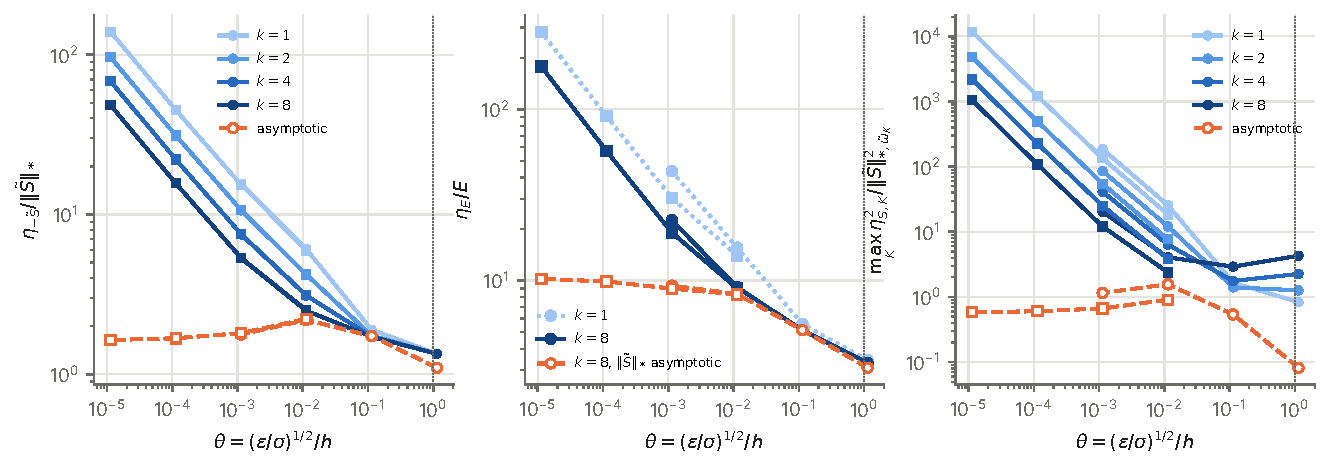
\includegraphics[width=\textwidth]{figures/sv_refref.pdf}
\caption{\asref{Reaction regime, layers problem, $n=16$, A+S estimator; circles $\sigma=1$, squares $\sigma=10^4$.
Left: $\eta_{-\Stil}/\|\Stil\|_*$ with $P_2$ references on $k$-times refined meshes and with the asymptotic value
\eqref{eq:Sasym}. Middle: $\eta_E/E$ with the same-mesh and the $8$ times refined references, and with
$\|\Stil\|_*$ from \eqref{eq:Sasym}. Right: the local ratio for $\ell=-\Stil$; the refined references are lower bounds
of the local dual norms, so these ratios are upper estimates; the asymptotic value is valid only for $\theta\ll1$.}}
\label{fig:refref}
\end{figure}

\begin{figure}[!htbp]
\centering
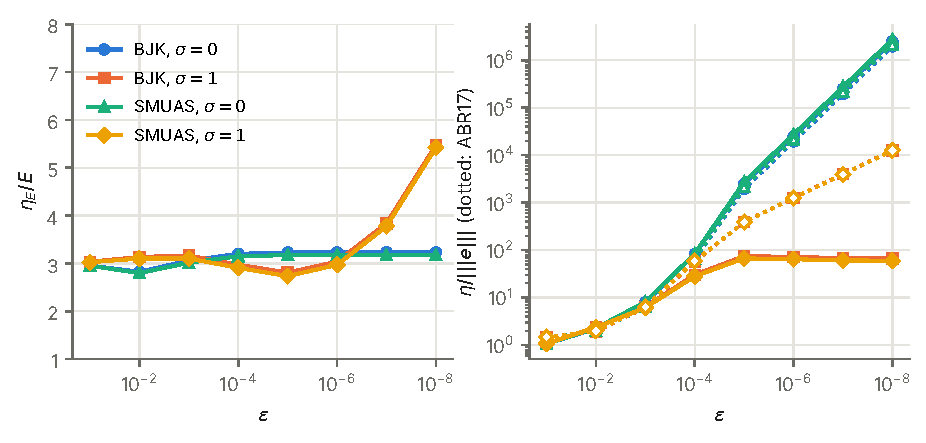
\includegraphics[width=\textwidth]{figures/sv_sweep.pdf}
\caption{Layers problem, $n=32$, as functions of $\eps$. Left: $I_E=\eta_E/E$. Right: the energy-norm
indices $\eta/\tnorm{e}$ (solid) and, dotted with open markers, that of the guaranteed bound of
\cite{ABR17}.}
\label{fig:sweep}
\end{figure}

\subsection{Variable reaction}\label{sec:num-cb}

With $c=1+(c_{\max}-1)xy$ and $\sigma=1$, the constant of (H3) is $\|c\|_\infty/\sigma=c_{\max}$, attained at
the vertex $(1,1)$. \refe{The computed $c_b$ is the sampled enclosure of Remark~\ref{rem:CF}, which is diagnostic: $c$ is not
affine on the cells, so the sampled maximum is enlarged by $\frac{h_K}2\max|\nabla c|$; here this gives} $c_b=1.12\,c_{\max}$, $1.06\,c_{\max}$
and $1.03\,c_{\max}$ for $n=8,16,32$, and $\kappa=2+c_b$ (Table~\ref{tab:cb}). The bound $E\le\eta_E$ holds in
all runs. The index of $\eta_{E,c}$ grows at most linearly, $\eta_{E,c}/E_c\le3\,c_b$ in all runs, as
Corollary~\ref{cor:twoc} predicts; it is often much smaller, down to $0.05\,c_b$, because the factor $M=c_b$ in front of $\tnorm{e}$ in $E_c$ also enlarges the
error measure. The index of $\eta_E$ grows faster, up to $5.2\,c_b$ at $c_b\approx10^3$, but stays far
below the worst case $(1+c_b)^2$ of Corollary~\ref{cor:two}. A variable reaction with a small lower
bound $\sigma$ is therefore the one situation in which the estimator loses its robustness, in
accordance with the theory; Section~\ref{sec:concl} discusses how to remove it.

% generated by examples/convection_diffusion/sv_numerics/make_figures.py; do not edit
\begin{table}[!htbp]
\centering
\small
\setlength{\tabcolsep}{4pt}
\caption{Variable reaction $c=1+(c_{\max}-1)xy$, $\sigma=1$, $\eps\in\{10^{-3},10^{-6}\}$, $n\in\{8,16,32\}$: ranges over the six runs; $c_b$ and $\kappa$ are the means of the sampled enclosures (Remark~\ref{rem:CF}; diagnostic), which exceed $c_{\max}$ by $3$--$12\,\%$.}\label{tab:cb}
\begin{tabular}{rrrllll}
\toprule
$c_{\max}$ & $c_b$ & $\kappa$ & $\eta_E/E$ & $\eta_{E,c}/E_c$ & $\eta_{E,c}/(c_bE_c)$ & $E\le\eta_E$\\
\midrule
1 & 1.00 & 3.00 & 3.85--5.34 & 3.85--5.34 & 3.85--5.34 & yes\\
10 & 10.66 & 12.66 & 14.63--19.94 & 8.69--30.35 & 0.85--2.95 & yes\\
100 & 107.22 & 109.22 & 128--271 & 12.27--216 & 0.12--2.09 & yes\\
1000 & $1.1\cdot10^{3}$ & $1.1\cdot10^{3}$ & 1618--5312 & 56.23--1125 & 0.05--1.09 & yes\\
\bottomrule
\end{tabular}
\end{table}


\subsection{Local efficiency}\label{sec:num-loc}

Table~\ref{tab:loc} reports the localised measure for the layers problem on the $16\times16$ mesh. The
local ratio $\max_K\eta_K^2/E_{\mathrm{loc}}(\tilde\omega_K)^2$ is at most $0.51$ in all cases, and
independent of $\eps$ for $\eps\le10^{-4}$: the estimator is locally efficient, as stated in
Theorem~\ref{thm:loc}. The ratio $E_{\mathrm{loc}}/E$ lies between $0.48$ and $1.01$, so on these
problems the localised measure captures most of the global one, and the guaranteed bound
$E_{\mathrm{loc}}\le\sqrt{d+1}\,\eta_E$ of Theorem~\ref{thm:loc} overestimates $E_{\mathrm{loc}}$ by a
factor $5$--$12$. The largest value, $\eta_E/E_{\mathrm{loc}}=7.0$ for $\sigma=1$ and $\eps=10^{-8}$, is the
same reference effect as in Section~\ref{sec:num-robust}.

% generated by examples/convection_diffusion/sv_numerics/make_figures.py; do not edit
\begin{table}[!htbp]
\centering
\small
\setlength{\tabcolsep}{4pt}
\caption{Localised measure (Theorem~\ref{thm:loc}), outflow layers, BJK, $n=16$. The last but one column is $\max_K\eta_K^2/E_{\mathrm{loc}}(\tilde\omega_K)^2$ with $\eta_K=\eta_{A,K}+\eta_{S,K}$.}\label{tab:loc}
\begin{tabular}{rrrrrrr}
\toprule
$\sigma$ & $\eps$ & $E_{\mathrm{loc}}/E$ & $\eta_E/E_{\mathrm{loc}}$ & $\sqrt{d+1}\,\eta_E/E_{\mathrm{loc}}$ & local max & $I_E$\\
\midrule
0 & $10^{-2}$ & 0.48 & 5.94 & 10.29 & 0.26 & 2.88\\
0 & $10^{-4}$ & 0.60 & 5.50 & 9.53 & 0.37 & 3.28\\
0 & $10^{-6}$ & 0.60 & 5.50 & 9.52 & 0.37 & 3.29\\
0 & $10^{-8}$ & 0.60 & 5.50 & 9.52 & 0.37 & 3.29\\
1 & $10^{-2}$ & 0.52 & 6.38 & 11.05 & 0.51 & 3.33\\
1 & $10^{-4}$ & 0.95 & 3.07 & 5.32 & 0.13 & 2.93\\
1 & $10^{-6}$ & 1.01 & 3.47 & 6.01 & 0.07 & 3.51\\
1 & $10^{-8}$ & 1.01 & 7.04 & 12.20 & 0.07 & 7.13\\
\bottomrule
\end{tabular}
\end{table}


\subsection{Adaptive refinement}\label{sec:num-adapt}

Starting from the $8\times8$ mesh, we mark by the indicators $\eta_K=\eta_{A,K}+\eta_{S,K}$ with the
dual strategy of \cite{AJ27} (all cells with $\eta_K\ge\theta\max\eta$, $\theta=0.5$, reduced until at least
$5\,\%$ of the cells are marked) and refine by red--green refinement, until $N>3\cdot10^4$.
Table~\ref{tab:adapt} and Figures~\ref{fig:adapt} and~\ref{fig:adaptmesh} show the results for the layers
problem.
\begin{itemize}
  \item \textbf{Effectivity.} $I_E$ stays between $2.86$ and $3.55$ in every loop of all three runs, from
  $N=81$ to $N=45\,094$, while the local mesh size spans three orders of magnitude.
  \item \textbf{Where the mesh is refined.} The refinement concentrates in the outflow layers at $x=1$ and
  $y=1$ (Figure~\ref{fig:adaptmesh}); the smallest cells have $h_{\min}=3.5\cdot10^{-4}$ for $\eps=10^{-3}$,
  below $\eps$, so the layers are resolved, and $h_{\min}=1.7\cdot10^{-4}$ for $\eps=10^{-5}$, where they are not.
  \item \textbf{Convergence.} For $\eps=10^{-3}$, $E$ decreases at the rate $1.8$--$1.9$ with respect to
  $N^{-1/2}$ over the second half of the loops: this is the pre-asymptotic phase in which the layers become
  resolved, faster than the optimal rate $1$. For $\eps=10^{-5}$ the rate is $0.98$. On the finest uniform mesh
  ($N=16\,641$) the error $E$ is $18$, $4.4$ and $17$ times larger than the adaptive error at the same $N$.
  Under uniform refinement $E$ decreases at the rate $0.46$--$0.60$ for $\sigma=0$ and $0.04$--$0.51$ for
  $\sigma=1$, because the layers are never resolved; the index $I_E$ is $2.86$--$3.37$ there as well.
  \item \textbf{Energy norm.} Along the adaptive runs the energy-norm index $I$ falls from $29$ to $1.1$
  ($\eps=10^{-3}$) and from $8.4\cdot10^3$ to $6.2$ ($\eps=10^{-5}$): once the mesh resolves the layers, the
  energy error and the dual norm of the residual become comparable, while $I_E$ is insensitive to this.
\end{itemize}

% generated by examples/convection_diffusion/sv_numerics/make_figures.py; do not edit
\begin{table}[!htbp]
\centering
\small
\setlength{\tabcolsep}{4pt}
\caption{Adaptive refinement for the outflow-layers problem, BJK, dual marking by the SV indicators $\eta_K$, red--green refinement. The rate is that of $E$ with respect to $N^{-1/2}$ over the second half of the loops; the last column is the ratio of $E$ on the finest uniform mesh ($N=16641$) to the adaptive $E$ at the same $N$.}\label{tab:adapt}
\begin{tabular}{rrrrllrlr}
\toprule
$\eps$ & $\sigma$ & loops & $N$ (last) & $h_{\min}$ & $E$ (last) & rate & $\eta_E/E$ & gain\\
\midrule
$10^{-3}$ & 0 & 15 & 33010 & $3.45\cdot10^{-4}$ & $7.395\cdot10^{-2}$ & 1.88 & 2.86--3.25 & 18.3\\
$10^{-5}$ & 0 & 12 & 31866 & $1.73\cdot10^{-4}$ & $3.941$ & 0.98 & 2.94--3.35 & 4.4\\
$10^{-3}$ & 1 & 17 & 45094 & $1.73\cdot10^{-4}$ & $5.891\cdot10^{-2}$ & 1.83 & 2.96--3.55 & 17.2\\
\bottomrule
\end{tabular}
\end{table}


\begin{figure}[!htbp]
\centering
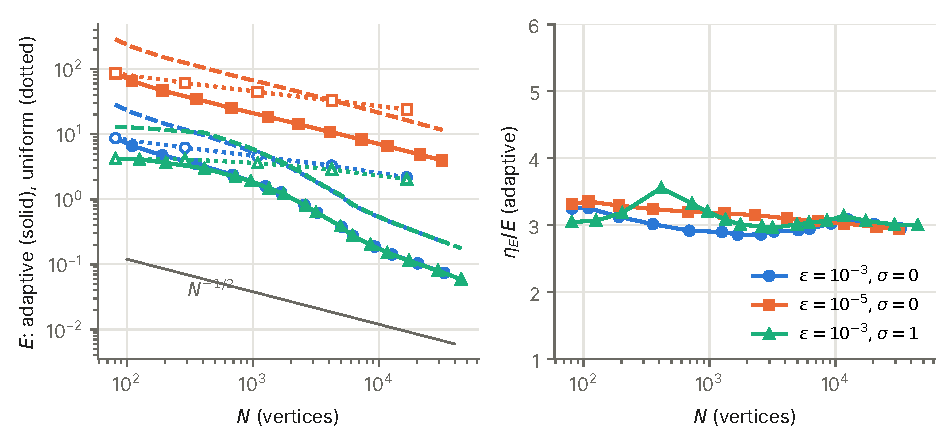
\includegraphics[width=\textwidth]{figures/sv_adapt.pdf}
\caption{Adaptive refinement, layers problem, BJK. Left: $E$ for adaptive (solid) and uniform (dotted, open
markers) refinement, and $\eta_E$ for the adaptive runs (dashed). Right: $I_E$ along the adaptive runs.}
\label{fig:adapt}
\end{figure}

\begin{figure}[!htbp]
\centering
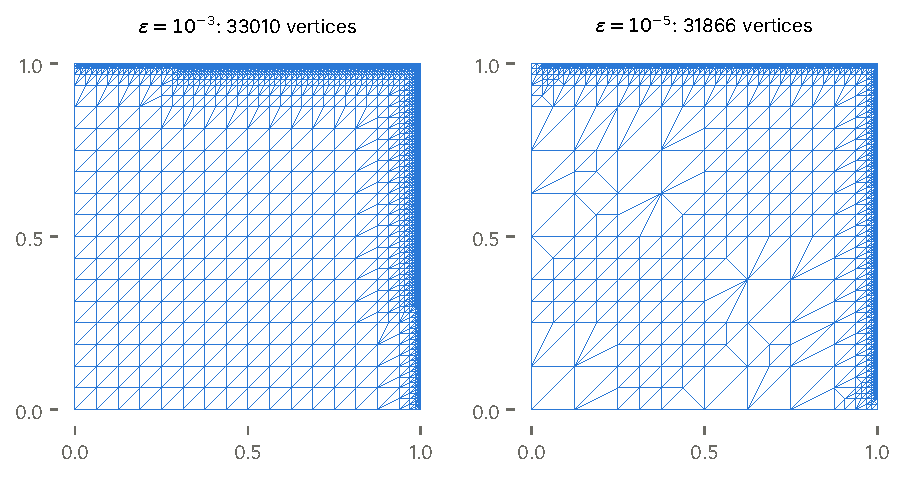
\includegraphics[width=\textwidth]{figures/sv_adapt_mesh.pdf}
\caption{Final adaptive meshes, layers problem, $\sigma=0$.}
\label{fig:adaptmesh}
\end{figure}

\subsection{\adapt{Uniform versus adaptive refinement}}\label{sec:num-unad}
{\color{magenta}

We repeat the uniform-mesh studies of Tables~\ref{tab:conv} and~\ref{tab:sweep} with adaptive refinement:
the same problems, the same marking as in Section~\ref{sec:num-adapt}, from the $8\times8$ mesh up to
$N\approx2\cdot10^4$ (Table~\ref{tab:conv}) and $N\approx10^4$ (Table~\ref{tab:sweep}). For the robustness
sweep we compare at equal cost: the adaptive loop whose $N$ is closest to $N=1089$, the size of the $32\times32$
mesh of Table~\ref{tab:sweep}.

\paragraph{Refinement studies (Figure~\ref{fig:aconv}).}
\begin{itemize}
  \item \textbf{Effectivity.} Along the adaptive runs $I_E$ lies in $2.83$--$4.18$ and tends to the same values
  as on uniform meshes, about $3.0$--$3.2$. The bound held in every loop.
  \item \textbf{Accuracy.} For the smooth solution, adaptive refinement gains nothing: at $N=16\,641$ the two
  errors agree to within $1\,\%$, and $E$ converges at the rate $1$ in both cases. For the layers problem the
  uniform error is $5.4$ ($\eps=10^{-2}$) and $5.9$ ($\eps=10^{-4}$) times the adaptive one at the same $N$.
  For $\eps=10^{-4}$, $E$ converges at the rate $0.47$ under uniform refinement and at $1.4$--$1.9$ in the last
  adaptive loops, in which the layers become resolved.
\end{itemize}

\begin{figure}[!htbp]
\centering
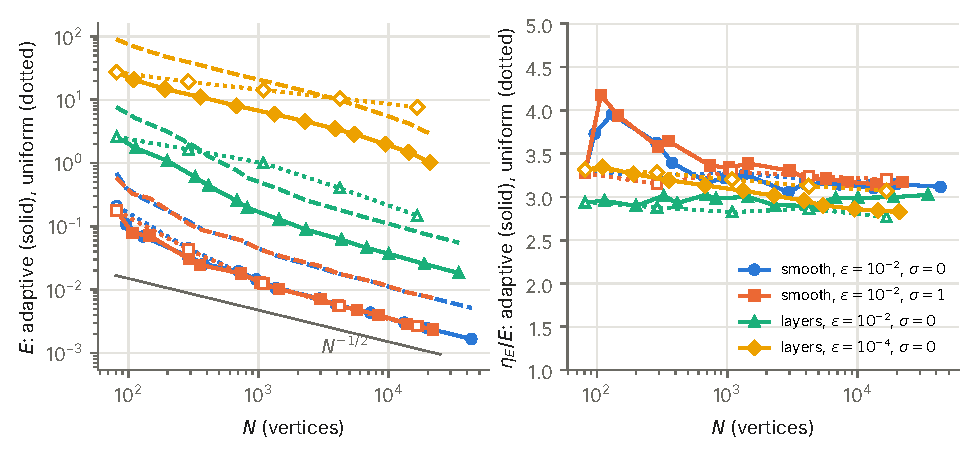
\includegraphics[width=\textwidth]{figures/sv_aconv.pdf}
\caption{\adapt{The cases of Table~\ref{tab:conv} under adaptive refinement. Left: $E$ for adaptive (solid) and uniform
(dotted, open markers) refinement, and $\eta_E$ for the adaptive runs (dashed). Right: $I_E$, adaptive (solid) and
uniform (dotted).}}
\label{fig:aconv}
\end{figure}

\paragraph{Robustness sweep (Figures~\ref{fig:abudget} and~\ref{fig:aloops}).}
\begin{itemize}
  \item \textbf{$\sigma=0$.} At equal cost, $I_E=2.89$--$3.22$ on the adaptive meshes against $2.80$--$3.23$ on the
  uniform mesh, for all $\eps$ and both stabilisations, and it stays in $2.82$--$3.35$ over all loops: the
  estimator is as robust on the meshes it generates as on the fixed mesh.
  \item \textbf{$\sigma=1$, small $\eps$.} The rise of $I_E$ to $5.4$--$5.5$ on the uniform mesh at
  $\eps\le10^{-7}$ (Section~\ref{sec:num-robust}) does not occur at equal cost on the adaptive meshes, where
  $I_E=2.75$--$3.16$. Figure~\ref{fig:aloops} shows why. The large values, up to $9.6$, appear only on the
  coarse initial mesh, and they come from the stabilisation part: $I_S=17.8$ at $N=81$ for $\eps=10^{-8}$. As the
  mesh resolves the layers, $I_S$ falls to $1.5$--$1.6$ and $I_E$ returns to about $3$. This confirms that the
  rise on the uniform mesh is a property of the under-resolved $P_2$ reference for $\|\Stil\|_*$, not of the
  estimator.
  \item \textbf{Smooth problem.} For $\eps\le10^{-3}$ the adaptive indices are higher than the uniform ones at
  equal cost: $I_E=4.0$--$5.3$ against $3.6$--$3.8$ for $\sigma=0$, and $4.5$--$6.0$ against $3.9$--$6.0$ for
  $\sigma=1$. Along the runs they reach $7.8$ after the first loop, and $10.9$ on the initial mesh. For $\sigma=1$
  and $\eps\le10^{-6}$ the fixed-point iteration reaches the iteration limit $2\cdot10^4$ on most meshes beyond
  $N\approx1100$, and the bound holds at these iterates.
  \item \textbf{Energy norm.} At $\sigma=0$ the energy-norm index still grows like $\eps^{-1}$ on the adaptive meshes,
  to $4\cdot10^5$ at $\eps=10^{-8}$ (uniform: $2.5\cdot10^6$); only the augmented measure is robust.
  \item \textbf{An open point.} For the layers problem with $\sigma=1$ and $\eps=10^{-6}$, $I_E$ rises again in the
  last loops, from $2.8$ to $4.3$, together with $I_\oplus$ (from $3.2$ to $6.6$). We have not identified the cause;
  it may be the convective part of the reference becoming resolved, and would need runs beyond $N=10^4$.
\end{itemize}

\begin{figure}[!htbp]
\centering
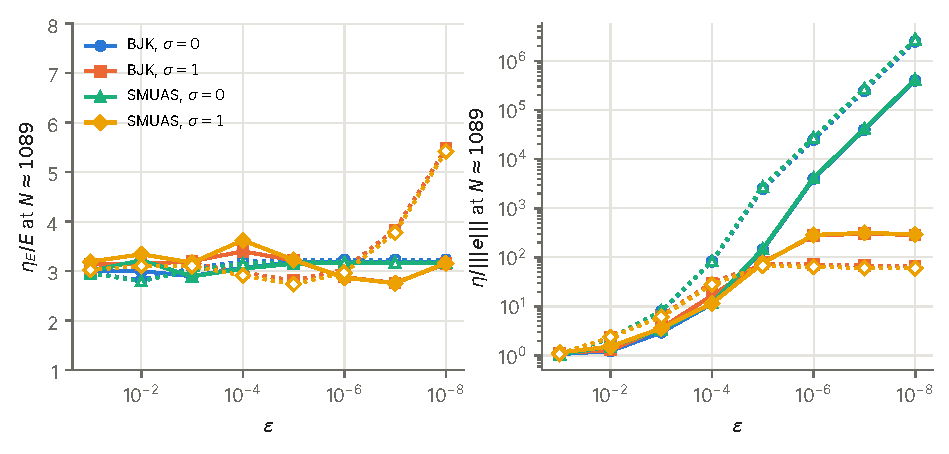
\includegraphics[width=\textwidth]{figures/sv_asweep_budget.pdf}
\caption{\adapt{The robustness sweep of Table~\ref{tab:sweep} at equal cost, layers problem: adaptive meshes with
$N\approx1089$ (solid) against the uniform $32\times32$ mesh (dotted, open markers). Left: $I_E$. Right: the
energy-norm index $\eta/\tnorm{e}$.}}
\label{fig:abudget}
\end{figure}

\begin{figure}[!htbp]
\centering
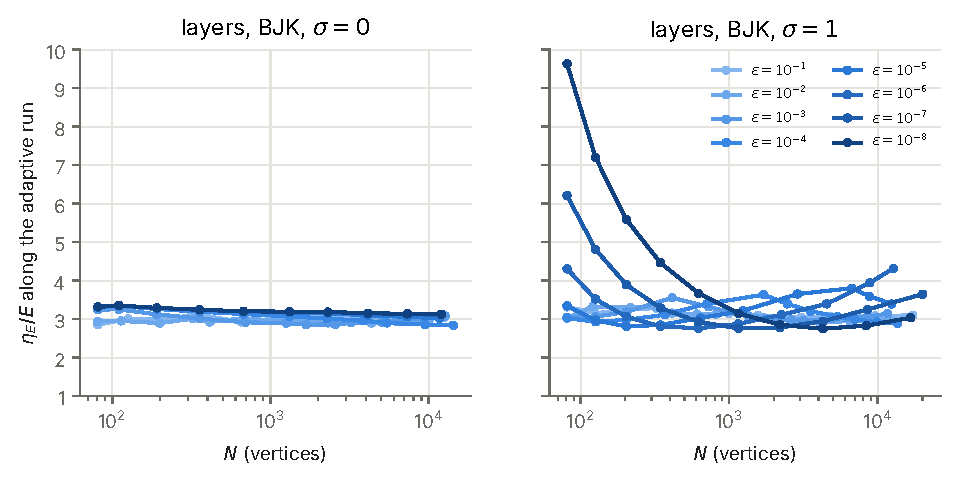
\includegraphics[width=\textwidth]{figures/sv_asweep_loops.pdf}
\caption{\adapt{$I_E$ along the adaptive runs of the robustness sweep, layers problem, BJK; one line per $\eps$, darker for
smaller $\eps$.}}
\label{fig:aloops}
\end{figure}

\paragraph{Which refinement to use.} For computing solutions, adaptive refinement is clearly preferable when the
solution has layers, by factors $4$--$18$ in $E$ at equal $N$, and it is what the estimator is designed for. For
testing the theory, the uniform meshes remain the primary evidence: a fixed coarse mesh keeps the layers
unresolved, which is the regime in which robustness can fail, isolates the dependence on $\eps$ and $\sigma$, and
is the only setting in which rates in $h$ are meaningful. The adaptive runs confirm that the effectivity stays at
about $3$ on the meshes the estimator generates itself.
}% end of the magenta block

\subsection{Inexact iterates and adaptive stopping}\label{sec:num-stop}

\paragraph{Iterates.} Table~\ref{tab:iter} and Figure~\ref{fig:iter} evaluate the estimator at the
fixed-point iterates $u^i$ on the $16\times16$ mesh. The index $I_E$ stays between $2.9$ and $5.3$ at
every iterate, including the first one, where the algebraic part $\eta_{\mathrm{alg}}$ is up to $71\,\%$
of $\eta_{\mathrm{disc}}$: this is part~2 of Proposition~\ref{prop:stop}, efficiency at every iterate
without any condition on the algebraic error. The ratio $\eta_{\mathrm{alg}}/\eta_{\mathrm{disc}}$
decreases monotonically for all problems except the smooth one with $\eps=10^{-6}$ and $\sigma=0$, for
which the fixed-point iteration does not converge in $2\cdot10^4$ iterations; there the ratio stalls
between $10^{-3}$ and $4\cdot10^{-3}$. In that case the error is smallest at $i\approx10$, $E(u^{10})=4.8$, and grows to
$8.4$ at $i=2\cdot10^4$: further iterations make the iterate worse in $E$, and the estimator, which is
efficient at every iterate, reflects this.

% generated by examples/convection_diffusion/sv_numerics/make_figures.py; do not edit
\begin{table}[!htbp]
\centering
\small
\setlength{\tabcolsep}{4pt}
\caption{Fixed-point iterates $u^i$, $i\in\{1,2,5,\dots,1000\}$ below the converged count, and the converged solution; BJK, $n=16$. The split is $\eta_{\mathrm{disc}}=\eta_E-\eta_{\mathrm{alg}}$.}\label{tab:iter}
\begin{tabular}{lrrrlrrl}
\toprule
problem & $\eps$ & $\sigma$ & it.\ to tol. & $\eta_E/E$ over $i$ & $\max_i\eta_{\mathrm{alg}}/\eta_{\mathrm{disc}}$ & $E(u^1)/E(u^{\mathrm{last}})$ & $E\le\eta_E$\\
\midrule
smooth & $10^{-2}$ & 0 & 39 & 3.24--3.63 & 0.71 & 1.81 & yes\\
smooth & $10^{-2}$ & 1 & 37 & 3.15--3.45 & 0.51 & 1.58 & yes\\
smooth & $10^{-6}$ & 0 & 20000 & 3.76--4.61 & 0.58 & 1.06 & yes\\
smooth & $10^{-6}$ & 1 & 664 & 4.42--5.28 & 0.19 & 1.20 & yes\\
layers & $10^{-2}$ & 0 & 47 & 2.88--2.97 & 0.02 & 1.01 & yes\\
layers & $10^{-2}$ & 1 & 45 & 3.32--3.33 & 0.01 & 1.01 & yes\\
layers & $10^{-6}$ & 0 & 635 & 3.29--3.47 & 0.04 & 1.01 & yes\\
layers & $10^{-6}$ & 1 & 502 & 3.51--3.56 & 0.02 & 1.03 & yes\\
\bottomrule
\end{tabular}
\end{table}


\begin{figure}[!htbp]
\centering
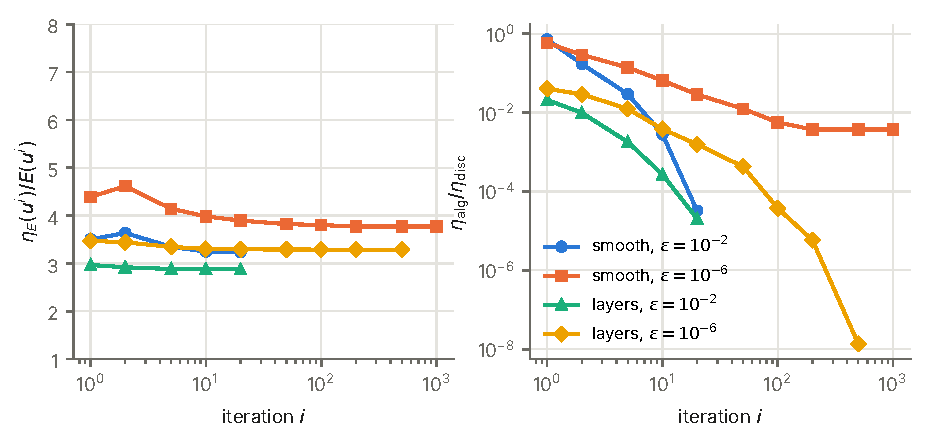
\includegraphics[width=\textwidth]{figures/sv_iter.pdf}
\caption{Fixed-point iterates, BJK, $\sigma=0$, $n=16$. Left: $I_E$ at the iterate $u^i$. Right: the
ratio $\eta_{\mathrm{alg}}/\eta_{\mathrm{disc}}$ (points with a ratio below $10^{-8}$ are omitted).}
\label{fig:iter}
\end{figure}

\paragraph{Adaptive stopping.} Table~\ref{tab:stop} runs five adaptive loops \refe{as in} Section~\ref{sec:num-adapt}
in which the fixed-point iteration is stopped either at the fixed tolerance $\|r\|\le10^{-10}\sqrt N$ or by
the criterion \eqref{eq:stop}, $\eta_{\mathrm{alg}}\le\gamma\eta_{\mathrm{disc}}$, with
$\eta_{\mathrm{disc}}=\eta_E-\eta_{\mathrm{alg}}$; each loop starts from the zero initial guess.
\begin{itemize}
  \item \textbf{Savings.} With $\gamma=0.1$, the total number of iterations drops from $227$ to $25$ (smooth,
  $\eps=10^{-2}$) and from $2323$ to $25$ (layers, $\eps=10^{-4}$), by factors $9$ and $93$; with $\gamma=0.01$
  the factors are $4.5$ and $46$.
  \item \textbf{Accuracy.} The final error $E$ changes by at most $6\,\%$ ($\gamma=0.1$, layers) and by at most
  $0.3\,\%$ for $\gamma\le0.01$. The index $I_E$ stays in $3.1$--$4.8$ in all runs, and in every stopped loop
  $\eta_{\mathrm{alg}}/\eta_{\mathrm{disc}}\le\gamma$, so $E\le(1+\gamma)\eta_{\mathrm{disc}}$
  (Proposition~\ref{prop:stop}, part~3).
  \item \textbf{Non-converging iteration.} For the smooth problem with $\eps=10^{-6}$ the fixed-point
  iteration does not reach the tolerance within $10^4$ iterations on any mesh, and $50\,000$ iterations give
  $E=3.22$. The criterion with $\gamma=0.1$ stops after $5$--$15$ iterations per loop, $50$ in total, with a
  \emph{smaller} error, $E=1.98$: as in Figure~\ref{fig:iter}, the early iterates are better than the late
  ones. For $\gamma=10^{-3}$ the criterion fires in only one of the five loops, since $\eta_{\mathrm{alg}}/\eta_{\mathrm{disc}}$ stalls
  at about $3\cdot10^{-3}$; this is a property of the iteration, not of the estimator.
\end{itemize}

% generated by examples/convection_diffusion/sv_numerics/make_figures.py; do not edit
\begin{table}[!htbp]
\centering
\footnotesize
\setlength{\tabcolsep}{4pt}
\caption{Adaptive stopping in five adaptive loops (dual marking by the SV indicators, red--green refinement), BJK, $\sigma=0$. ``tol.'' is the fixed tolerance $\|r\|\le10^{-10}\sqrt N$; otherwise the iteration stops at $\eta_{\mathrm{alg}}\le\gamma\eta_{\mathrm{disc}}$ (at most $10^4$ iterations). The last column says whether every loop stopped before the iteration limit.}\label{tab:stop}
\begin{tabular}{lrrrrlllr}
\toprule
problem & $\eps$ & $\gamma$ & it./loop & total & $E$ (last) & $\eta_E/E$ & $\max\eta_{\mathrm{alg}}/\eta_{\mathrm{disc}}$ & stopped\\
\midrule
smooth & $10^{-2}$ & tol. & 30--59 & 227 & $2.550\cdot10^{-2}$ & 3.29--3.95 & $5.78\cdot10^{-8}$ & yes\\
smooth & $10^{-2}$ & 0.1 & 5 & 25 & $2.554\cdot10^{-2}$ & 3.41--3.97 & $5.07\cdot10^{-2}$ & yes\\
smooth & $10^{-2}$ & 0.01 & 10 & 50 & $2.551\cdot10^{-2}$ & 3.33--3.98 & $7.27\cdot10^{-3}$ & yes\\
smooth & $10^{-2}$ & 0.001 & 10--20 & 80 & $2.551\cdot10^{-2}$ & 3.29--3.96 & $9.89\cdot10^{-4}$ & yes\\
smooth & $10^{-6}$ & tol. & 10000 & 50000 & $3.218$ & 3.77--4.58 & $3.03\cdot10^{-3}$ & no\\
smooth & $10^{-6}$ & 0.1 & 5--15 & 50 & $1.984$ & 4.04--4.79 & $9.83\cdot10^{-2}$ & yes\\
smooth & $10^{-6}$ & 0.01 & 120--760 & 2190 & $2.749$ & 3.80--4.45 & $9.10\cdot10^{-3}$ & yes\\
smooth & $10^{-6}$ & 0.001 & 7320--10000 & 47320 & $3.218$ & 3.77--4.58 & $3.03\cdot10^{-3}$ & no\\
layers & $10^{-4}$ & tol. & 385--628 & 2323 & $8.044$ & 3.13--3.34 & $3.57\cdot10^{-9}$ & yes\\
layers & $10^{-4}$ & 0.1 & 5 & 25 & $8.524$ & 3.20--3.42 & $2.49\cdot10^{-2}$ & yes\\
layers & $10^{-4}$ & 0.01 & 10 & 50 & $8.023$ & 3.15--3.38 & $8.43\cdot10^{-3}$ & yes\\
layers & $10^{-4}$ & 0.001 & 25--50 & 175 & $8.04$ & 3.14--3.35 & $9.29\cdot10^{-4}$ & yes\\
\bottomrule
\end{tabular}
\end{table}


\subsection{Variable diffusion}\label{sec:num-vareps}

Table~\ref{tab:vareps} reports the variable-diffusion problems on the meshes $n=8,16,32$. All bounds are
guaranteed. For the smooth coefficient, the oscillation $\eta_\eps$ converges at the rate $2.09$--$2.13$
in $h$, in accordance with Lemma~\ref{lem:V}(iii), and is at most $12\,\%$ of $\eta$ (at contrast $10^4$ on
the coarsest mesh). For the jump aligned with the mesh, $\Pi_1\eps=\eps$ and $\eta_\eps=0$. The
effectivity $I_E$ lies in $2.6$--$4.5$ for contrasts up to $10^4$, for $\eps=10^{-2}$ and $10^{-6}$ alike. For
the jump it does not grow with the contrast; for the smooth coefficient it grows mildly, from
$3.1$ at contrast $1$ to at most $4.3$ at contrast $10^4$ (on the coarsest mesh). This is the quasi-monotone case; the constants of
Theorem~\ref{thm:vareps} depend on the patch contrast, but for an aligned jump that contrast does not
show up in the indices. Checkerboard (non-quasi-monotone) coefficients are not tested; for them no
local estimator can be robust \cite{Li26}.

% generated by examples/convection_diffusion/sv_numerics/make_figures.py; do not edit
\begin{table}[!htbp]
\centering
\footnotesize
\setlength{\tabcolsep}{4pt}
\caption{Variable diffusion, BJK, $\sigma=0$, $n\in\{8,16,32\}$: ranges over the three meshes. The rate is that of $\eta_\eps$ with respect to $N^{-1/2}$ between $n=16$ and $n=32$ (expected: $2$).}\label{tab:vareps}
\begin{tabular}{lrrllllrl}
\toprule
$\eps(x)$ & $\eps$ & contrast & $I$ & $I_\oplus$ & $I_E$ & $\max\eta_\eps/\eta$ & rate & $E\le\eta_E$\\
\midrule
smooth & $10^{-2}$ & 1 & 1.23--4.58 & 3.30--4.06 & 3.07--3.13 & 0.000 & --- & yes\\
smooth & $10^{-2}$ & 100 & 1.07--1.24 & 3.16--3.39 & 3.15--3.26 & 0.035 & 2.09 & yes\\
smooth & $10^{-2}$ & 10000 & 1.10--1.44 & 3.30--4.28 & 3.29--4.27 & 0.117 & 2.09 & yes\\
smooth & $10^{-6}$ & 1 & 7959--36796 & 3.72--5.01 & 3.50--3.70 & 0.000 & --- & yes\\
smooth & $10^{-6}$ & 100 & 818--3354 & 3.73--5.44 & 3.54--4.03 & 0.000 & 2.13 & yes\\
smooth & $10^{-6}$ & 10000 & 64.07--336 & 4.31--5.49 & 3.94--4.46 & 0.001 & 2.10 & yes\\
jump & $10^{-2}$ & 100 & 2.56--7.63 & 3.43--4.18 & 2.61--2.99 & 0.000 & --- & yes\\
jump & $10^{-2}$ & 10000 & 2.61--8.12 & 3.43--4.22 & 2.60--3.01 & 0.000 & --- & yes\\
jump & $10^{-6}$ & 100 & 9025--28125 & 4.75--5.12 & 3.44--3.54 & 0.000 & --- & yes\\
jump & $10^{-6}$ & 10000 & 2156--4989 & 4.78--5.08 & 3.41--3.52 & 0.000 & --- & yes\\
\bottomrule
\end{tabular}
\end{table}


\subsection{Three dimensions}\label{sec:num-3d}

Table~\ref{tab:d3} repeats the uniform-refinement study on the unit cube ($n=4,8,16$, up to $N=4913$
vertices and $24\,576$ tetrahedra).
\begin{itemize}
  \item \textbf{Layers.} $I_E=2.94$--$3.55$ for $\eps=10^{-2}$ and $10^{-6}$, as in two dimensions; $I_\oplus\le4.9$
  and $I_S=1.21$--$1.26$.
  \item \textbf{Smooth solution.} $I_E$ is higher than in two dimensions, $5.1$--$6.4$, but decreases under
  refinement for both values of $\eps$ ($5.97\to5.40$ and $6.39\to5.09$). These meshes are coarse: $E$ still
  converges at the pre-asymptotic rates $2.1$--$2.7$ in $h$, dominated by the stabilisation part
  $\|\Stil\|_*$, which is estimated sharply ($I_S=1.28$--$1.31$); the larger index comes from the convective
  dual norm on coarse tetrahedral meshes. For $\eps=10^{-6}$ on the finest mesh the fixed-point iteration does
  not converge within $2\cdot10^4$ iterations, and the bound still holds at the last iterate.
  \item \textbf{Energy norm.} As in two dimensions, $I$ is useless for $\sigma=0$ and small $\eps$
  ($1.0\cdot10^4$--$1.4\cdot10^5$ at $\eps=10^{-6}$, against $2.6$--$9.3$ at $\eps=10^{-2}$), while $I_E$ is not
  affected.
  \item \textbf{Cost.} The estimator takes about $8$\,s at $N=729$ and $220$--$240$\,s at $N=4913$ in our
  Python implementation; the cost is dominated by the vertex-patch problems in $\RTN$, whose size grows
  quickly with the number of tetrahedra per patch in three dimensions. The patch problems are independent and
  can be solved in parallel; the global $\RT_0$ defect problem takes a small fraction of the time.
\end{itemize}

% generated by examples/convection_diffusion/sv_numerics/make_figures.py; do not edit
\begin{table}[!htbp]
\centering
\small
\setlength{\tabcolsep}{4pt}
\caption{Three dimensions, uniform refinement of the unit cube, BJK, $\sigma=0$. Rates with respect to $N^{-1/3}\sim h$; the last column is the time of the estimator in seconds.}\label{tab:d3}
\begin{tabular}{lrrlrrrrr}
\toprule
problem & $\eps$ & $N$ & $E$ & rate & $I$ & $I_\oplus$ & $I_E$ & time\\
\midrule
smooth & $10^{-2}$ & 125 & $0.7$ &  & 9.27 & 7.82 & 5.97 & 0.7\\
smooth & $10^{-2}$ & 729 & $0.144$ & 2.69 & 4.83 & 6.98 & 5.71 & 9.0\\
smooth & $10^{-2}$ & 4913 & $3.55\cdot10^{-2}$ & 2.20 & 2.64 & 5.84 & 5.40 & 226.6\\
smooth & $10^{-6}$ & 125 & $6.72\cdot10^{1}$ &  & $7.4\cdot10^{4}$ & 9.26 & 6.39 & 0.6\\
smooth & $10^{-6}$ & 729 & $2.00\cdot10^{1}$ & 2.06 & $2.8\cdot10^{4}$ & 6.93 & 5.31 & 8.4\\
smooth & $10^{-6}$ & 4913 & $4.06$ & 2.51 & $1.0\cdot10^{4}$ & 5.56 & 5.09 & 238.0\\
layers & $10^{-2}$ & 125 & $2.74$ &  & 6.67 & 4.01 & 3.10 & 0.6\\
layers & $10^{-2}$ & 729 & $1.82$ & 0.70 & 4.31 & 3.71 & 3.01 & 8.0\\
layers & $10^{-2}$ & 4913 & $1.14$ & 0.73 & 2.93 & 3.64 & 2.94 & 217.3\\
layers & $10^{-6}$ & 125 & $2.79\cdot10^{2}$ &  & $1.4\cdot10^{5}$ & 4.71 & 3.38 & 0.5\\
layers & $10^{-6}$ & 729 & $2.01\cdot10^{2}$ & 0.56 & $7.3\cdot10^{4}$ & 4.78 & 3.47 & 8.5\\
layers & $10^{-6}$ & 4913 & $1.35\cdot10^{2}$ & 0.63 & $3.8\cdot10^{4}$ & 4.93 & 3.55 & 236.1\\
\bottomrule
\end{tabular}
\end{table}


\subsection{Summary}

The experiments answer the questions (Q1)--(Q7) as follows.
\begin{enumerate}[label=(Q\arabic*)]
  \item The bound $E\le\eta_E$ held in every run: two and three dimensions, both stabilisations,
  $\eps=10^{-1},\dots,10^{-8}$, $\sigma\in\{0,1\}$, variable reaction and diffusion, adaptive meshes and inexact
  iterates\refe{, and so did $I\ge1$, $I_\oplus\ge1$ and $I_S\ge1$. Since the references are lower bounds of the dual
  norms, this is a consistency check rather than a proof}.
  \item For constant coefficients, $I_E$ lies in $2.6$--$5.3$ in two dimensions, inexact iterates included,
  independently of $\eps$, $\sigma$, the stabilisation and the mesh; the only exception is a rise to $6.0$
  ($n=32$) and $7.1$ ($n=16$) at $\sigma=1$, $\eps\le10^{-7}$, \adapt{which the adaptive runs identify as an
  under-resolved reference for $\|\Stil\|_*$ (Section~\ref{sec:num-unad})}\asref{, as the asymptotically exact
  reference \eqref{eq:Sasym} confirms ($I_S=1.6$--$2.2$ and $\eta_E/E=8.3$--$10.2$ for $\theta$ down to $10^{-5}$)}; in three dimensions it is $2.9$--$6.4$ and
  decreases under refinement. The energy-norm index $I$, and the guaranteed bound of \cite{ABR17}, are not
  robust.
  \item The effectivity grows with $c_b$, at most linearly for $\eta_{E,c}$ and well below $c_b^2$ for $\eta_E$:
  a variable reaction with a small lower bound is the one case in which robustness is lost, as the theory
  predicts.
  \item The local ratio $\max_K\eta_K^2/E_{\mathrm{loc}}(\tilde\omega_K)^2$ is at most $0.51$.
  \item Adaptive refinement driven by $\eta_K$ resolves the layers and reduces $E$ by factors $4$--$18$
  against uniform refinement at equal $N$, with $I_E=2.9$--$3.6$ throughout. \adapt{Repeating the refinement and
  robustness studies adaptively gives the same effectivity, about $3$, as on uniform meshes.}
  \item The estimator is efficient at every iterate, and the stopping criterion saves up to $99\,\%$ of the
  iterations at a change of the error of at most $6\,\%$ ($\gamma=0.1$) or $0.3\,\%$ ($\gamma\le0.01$).
  \item For variable diffusion, $\eta_\eps$ converges at rate $2$ and $I_E$ stays in $2.6$--$4.5$ up to contrast
  $10^4$.
\end{enumerate}

\paragraph{Reproducibility.} All results are produced by the scripts \texttt{run\_numerics.py} and
\texttt{make\_figures.py} in the directory
\path{examples/convection_diffusion/sv_numerics} of \texttt{galerkit}. The first runs the experiments (about
$35$ minutes on four cores, the three-dimensional runs sequentially because of their memory use); the
second writes the tables, the figures and, for every stored solution, a VTK file
(\texttt{.vtu}) with $u_h$, $u$, $u-u_h$, $\eps$, $\eta_K$, $\tnorm{e}_K$ and the local effectivity
$\eta_K/\tnorm{e}_K$. \adapt{The figures of Section~\ref{sec:num-unad} are produced by
\texttt{make\_adaptive\_figures.py} in the same directory.}

).
% Data: examples/convection_diffusion/sv_numerics/run_numerics.py (output/*.json);
% tables and figures: make_figures.py -> tables/*.tex, figures/sv_*.{pdf,png}.
% All numbers quoted in the text below are read off those tables.

% ===========================================================================
\section{Numerical experiments}\label{sec:num}
% ===========================================================================

We test the estimator against the exact error. The questions are the ones raised by the theory:
\begin{enumerate}[label=(Q\arabic*)]
  \item Is the bound guaranteed, $E\le\eta_E$, in every run (Theorem~\ref{thm:rel})?
  \item Are the effectivity indices bounded independently of $\eps$, $\sigma$ and the stabilisation
  (Theorem~\ref{thm:eff}, Corollary~\ref{cor:two}), and do they stay bounded under refinement?
  \item Does the dependence on $c_b$ follow Corollaries~\ref{cor:two} and~\ref{cor:twoc}?
  \item Is the estimator locally efficient in the localisable measure (Theorem~\ref{thm:loc})?
  \item Do the indicators drive adaptive refinement to the optimal rate?
  \item Are the bounds valid at inexact iterates, and does the stopping criterion of
  Proposition~\ref{prop:stop} save iterations without spoiling the error?
  \item Does the variable-diffusion version keep its effectivity, with $\eta_\eps=O(h^2)$
  (Theorem~\ref{thm:vareps})?
\end{enumerate}

\subsection{Setup}

\paragraph{Discretisation.} Conforming $P_1$ elements on uniform meshes of the unit square
($n\times n$ squares, each cut into two triangles; $N=(n+1)^2$ vertices) or the unit cube ($n^3$
cubes, each cut into six tetrahedra), and on red--green refined meshes in the adaptive runs. The
stabilisations are the AFC scheme with the limiter of \cite{BJK17} (BJK), and the symmetrised
monotone upwind-type algebraic stabilisation of \cite{Kn23} (SMUAS). The nonlinear problem is solved
by the damped fixed-point iteration of \cite{AJ27} up to $\|r\|\le10^{-10}\sqrt N$, with at most
$2\cdot10^4$ iterations, unless stated otherwise.

\paragraph{Test problems} (all with $b$ constant, so $\sigma=c$, $c_b=1$ and $\kappa=3$, except in
Section~\ref{sec:num-cb}).
\begin{itemize}
  \item \emph{smooth}: $u=\prod_i\sin(\pi x_i)+x_1^2\prod_{i>1}x_i$, $b=(1,\tfrac12)$ or
  $(1,\tfrac12,\tfrac14)$, Dirichlet data on $\partial\Omega$; $f$ is computed from $u$. The solution
  has no layers, so its error is not dominated by layers, but for small $\eps$ the scheme is
  convection-dominated on every mesh used.
  \item \emph{layers}: $u=\prod_iw(x_i)$ with
  $w(s)=s-\bigl(e^{(s-1)/\eps}-e^{-1/\eps}\bigr)/\bigl(1-e^{-1/\eps}\bigr)$, $b=(1,\dots,1)$, homogeneous
  Dirichlet data; $u$ has exponential layers of width $\eps$ at the outflow boundary $x_i=1$.
  \item \emph{variable diffusion}: $u=\phi(x_1)\prod_{i>1}4x_i(1-x_i)$, either with
  $\eps(x)=\eps\,k^{x_1}$, $\phi(s)=4s(1-s)$ (\emph{smooth}), or with $\eps$ jumping from $\eps$ to $k\eps$
  at $x_1=\frac12$ and $\phi$ chosen such that the flux $\eps\phi'$ is continuous (\emph{jump}); $k$ is
  the contrast.
\end{itemize}

\paragraph{Error measures.} $\tnorm{e}$ is computed with a quadrature of degree~8. The dual norms
$\|B_A'(e,\cdot)\|_*$ and $\|\Stil\|_*$, and the local dual norms of $E_{\mathrm{loc}}$, are computed
from their Riesz representatives in the $P_2$ space on the same mesh (on each vertex patch for
$E_{\mathrm{loc}}$). These are \emph{lower} bounds of the true dual norms, so the reported effectivity
indices are slight overestimates; they become crude when the dual norm concentrates in layers that
the mesh does not resolve (see Section~\ref{sec:num-robust}). We report the effectivity indices
\[
  I=\frac{\eta}{\tnorm{e}},\qquad I_\oplus=\frac{\kappa\eta}{\tnorm{e}_\oplus},\qquad
  I_S=\frac{\eta_S}{\|\Stil\|_*},\qquad I_E=\frac{\eta_E}{E},
\]
of which $I_E$ is the one covered by Corollary~\ref{cor:two}; $I_\oplus\ge1$ and $I\ge1$ are guaranteed
too, but only $I_\oplus$ is expected to be robust.

\subsection{Solutions and indicators}

Figure~\ref{fig:snap} shows the discrete solution of the layers problem for $\eps=10^{-3}$ on the
$32\times32$ mesh, the cell indicators $\eta_K=\eta_{A,K}+\eta_{S,K}$, and the local energy errors
$\tnorm{e}_K$. The mesh does not resolve the layers ($h\approx4.4\cdot10^{-2}\gg\eps$); the AFC
solution is free of oscillations, and both the indicators and the error concentrate in the cells at
the outflow boundary, with a decay of several orders of magnitude into the interior. The indicator
is larger than $\tnorm{e}_K$ in the layer cells: it measures the residual in the dual norm, which
contains the convective part $\|B_A'(e,\cdot)\|_*$ of the error.

\begin{figure}[!htbp]
\centering
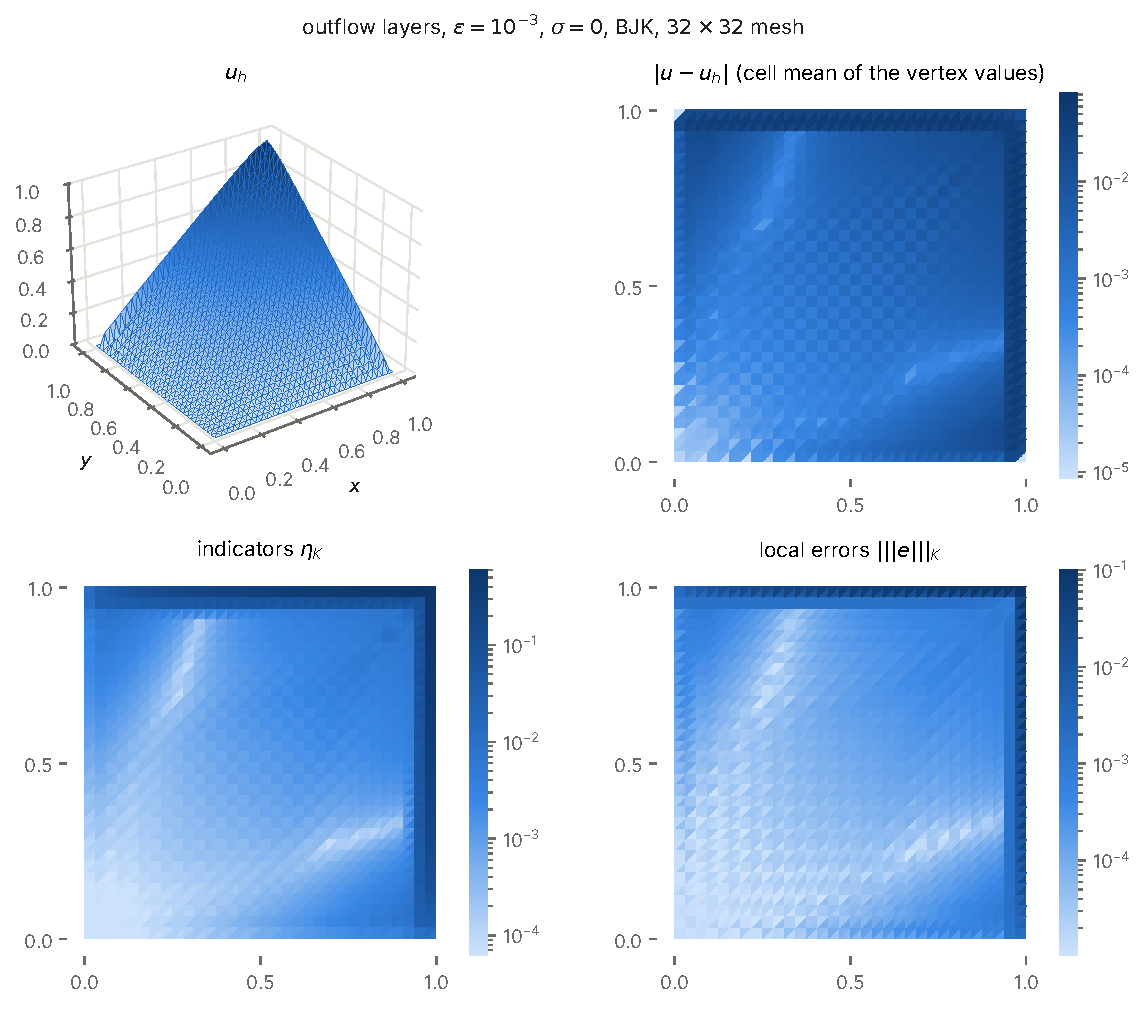
\includegraphics[width=\textwidth]{figures/sv_snap.pdf}
\caption{Layers problem, $\eps=10^{-3}$, $\sigma=0$, BJK, $n=32$: discrete solution $u_h$, indicators
$\eta_K$ and local errors $\tnorm{e}_K$ (logarithmic colour scale, common to both).}
\label{fig:snap}
\end{figure}

\subsection{Uniform refinement}\label{sec:num-conv}

Table~\ref{tab:conv} and Figure~\ref{fig:conv} report uniform refinement from $n=8$ to $n=128$.
\begin{itemize}
  \item \textbf{Smooth solution, $\eps=10^{-2}$.} $E$ and $\eta_E$ converge at the optimal rate $1$ in
  $h$ once the mesh resolves the solution; on the coarse meshes both decrease faster, because the
  stabilisation term $\|\Stil\|_*$ dominates $E$ there and decreases at a higher rate. The effectivity
  $I_E$ lies between $3.15$ and $3.29$ for $\sigma=0$ and $\sigma=1$ alike. The energy-norm index $I$
  tends to $1.1$: in the diffusion-dominated regime the energy norm and the dual norm of the
  residual coincide asymptotically.
  \item \textbf{Layers, $\eps=10^{-2}$.} The layers are resolved only from $n=64$ on, and the
  convergence of $E$ accelerates accordingly; $I_E$ stays between $2.77$ and $2.94$.
  \item \textbf{Layers, $\eps=10^{-4}$.} The meshes never resolve the layers. The energy error
  $\tnorm{e}$ \emph{increases} under refinement, because the error, concentrated in the outflow
  cells, sees an increasing part of the layer, while $E$ is dominated by the convective dual norm and
  decreases at the rate $0.45$--$0.53$; $\eta_E$ follows it with the rate $0.49$--$0.55$. The index $I_E$
  is $3.07$--$3.31$ on every mesh, whereas the energy-norm index $I$ falls from $833$ to $18.7$: the
  energy-norm bound is guaranteed but useless in this regime, which is why the error is measured in
  $E$.
\end{itemize}

% generated by examples/convection_diffusion/sv_numerics/make_figures.py; do not edit
\begin{table}[!htbp]
\centering
\small
\setlength{\tabcolsep}{4pt}
\caption{Uniform refinement in 2D, BJK. Rates with respect to $N^{-1/2}\sim h$; the expected rate is $1$ once the mesh resolves the solution. Effectivity indices $I=\eta/\tnorm{e}$, $I_\oplus=\kappa\eta/\tnorm{e}_\oplus$, $I_E=\eta_E/E$; the last column is the number of fixed-point iterations.}\label{tab:conv}
\begin{tabular}{rlllrlrrrr}
\toprule
$N$ & $\tnorm{e}$ & $E$ & rate & $\eta_E$ & rate & $I$ & $I_\oplus$ & $I_E$ & it.\\
\midrule
\multicolumn{10}{l}{\emph{smooth, $\eps=10^{-2}$, $\sigma=0$}}\\
81 & $4.88\cdot10^{-2}$ & $0.209$ &  & $0.687$ &  & 4.12 & 4.22 & 3.29 & 59\\
289 & $2.15\cdot10^{-2}$ & $4.48\cdot10^{-2}$ & 2.42 & $0.145$ & 2.45 & 2.05 & 3.86 & 3.24 & 39\\
1089 & $1.04\cdot10^{-2}$ & $1.26\cdot10^{-2}$ & 1.91 & $4.15\cdot10^{-2}$ & 1.89 & 1.31 & 3.46 & 3.28 & 18\\
4225 & $5.16\cdot10^{-3}$ & $5.51\cdot10^{-3}$ & 1.23 & $1.76\cdot10^{-2}$ & 1.26 & 1.14 & 3.24 & 3.20 & 9\\
16641 & $2.58\cdot10^{-3}$ & $2.65\cdot10^{-3}$ & 1.07 & $8.40\cdot10^{-3}$ & 1.08 & 1.09 & 3.18 & 3.17 & 6\\
\multicolumn{10}{l}{\emph{smooth, $\eps=10^{-2}$, $\sigma=1$}}\\
81 & $5.01\cdot10^{-2}$ & $0.178$ &  & $0.582$ &  & 3.34 & 4.04 & 3.27 & 56\\
289 & $2.16\cdot10^{-2}$ & $4.31\cdot10^{-2}$ & 2.23 & $0.136$ & 2.29 & 1.89 & 3.69 & 3.15 & 37\\
1089 & $1.04\cdot10^{-2}$ & $1.25\cdot10^{-2}$ & 1.87 & $4.12\cdot10^{-2}$ & 1.80 & 1.29 & 3.46 & 3.29 & 18\\
4225 & $5.16\cdot10^{-3}$ & $5.47\cdot10^{-3}$ & 1.22 & $1.77\cdot10^{-2}$ & 1.24 & 1.15 & 3.29 & 3.24 & 9\\
16641 & $2.58\cdot10^{-3}$ & $2.64\cdot10^{-3}$ & 1.06 & $8.45\cdot10^{-3}$ & 1.08 & 1.10 & 3.22 & 3.20 & 6\\
\multicolumn{10}{l}{\emph{layers, $\eps=10^{-2}$, $\sigma=0$}}\\
81 & $0.522$ & $2.6$ &  & $7.62$ &  & 4.19 & 3.78 & 2.94 & 67\\
289 & $0.471$ & $1.64$ & 0.72 & $4.72$ & 0.75 & 2.88 & 3.64 & 2.88 & 47\\
1089 & $0.366$ & $1$ & 0.74 & $2.83$ & 0.77 & 2.21 & 3.56 & 2.82 & 63\\
4225 & $0.231$ & $0.401$ & 1.35 & $1.15$ & 1.33 & 1.52 & 3.26 & 2.86 & 28\\
16641 & $0.127$ & $0.148$ & 1.46 & $0.409$ & 1.51 & 1.07 & 2.77 & 2.77 & 9\\
\multicolumn{10}{l}{\emph{layers, $\eps=10^{-4}$, $\sigma=0$}}\\
81 & $3.07\cdot10^{-2}$ & $2.72\cdot10^{1}$ &  & $9.02\cdot10^{1}$ &  & 833.01 & 4.76 & 3.31 & 405\\
289 & $6.15\cdot10^{-2}$ & $1.94\cdot10^{1}$ & 0.53 & $6.37\cdot10^{1}$ & 0.55 & 290.45 & 4.81 & 3.28 & 709\\
1089 & $0.154$ & $1.42\cdot10^{1}$ & 0.47 & $4.56\cdot10^{1}$ & 0.51 & 82.17 & 4.75 & 3.20 & 700\\
4225 & $0.242$ & $1.05\cdot10^{1}$ & 0.45 & $3.27\cdot10^{1}$ & 0.49 & 37.26 & 4.65 & 3.12 & 626\\
16641 & $0.342$ & $7.6$ & 0.47 & $2.33\cdot10^{1}$ & 0.49 & 18.72 & 4.54 & 3.07 & 566\\
\bottomrule
\end{tabular}
\end{table}


\begin{figure}[!htbp]
\centering
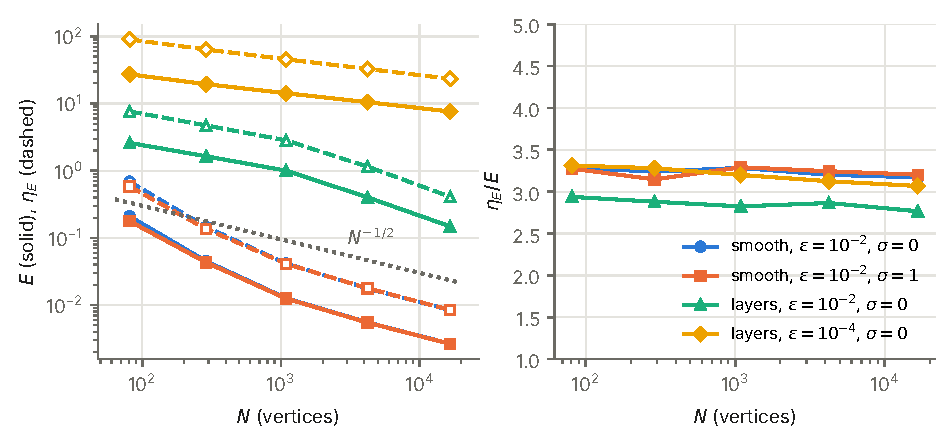
\includegraphics[width=\textwidth]{figures/sv_conv.pdf}
\caption{Uniform refinement in 2D, BJK. Left: $E$ (solid) and $\eta_E$ (dashed, open markers).
Right: effectivity index $I_E=\eta_E/E$.}
\label{fig:conv}
\end{figure}

\subsection{Robustness in \texorpdfstring{$\eps$}{eps}, \texorpdfstring{$\sigma$}{sigma} and the stabilisation}\label{sec:num-robust}

Table~\ref{tab:sweep} and Figure~\ref{fig:sweep} sweep $\eps$ from $10^{-1}$ to $10^{-8}$ on the fixed
mesh $n=32$, for $\sigma\in\{0,1\}$, both stabilisations and both problems.
\begin{itemize}
  \item \textbf{$\sigma=0$.} $I_E$ lies in $2.80$--$3.23$ for the layers problem and in $3.15$--$3.78$
  for the smooth problem, and becomes constant for $\eps\le10^{-5}$. $I_\oplus$ stays below $4.9$,
  and the stabilisation part is estimated sharply, $I_S=1.21$--$1.34$. BJK and SMUAS give the
  same indices $I_E$ and $I_\oplus$ to within $3\,\%$, as Remark~\ref{rem:robust} predicts: the limiter enters only
  through the functional, not the constants.
  \item \textbf{Energy norm.} The energy-norm index $I$ grows like $\eps^{-1}$ for $\sigma=0$, up to
  $2.5\cdot10^6$ at $\eps=10^{-8}$; the guaranteed energy-norm bound of \cite{ABR17} behaves in the
  same way. For $\sigma=1$, $I$ saturates at about $60$--$90$, the reaction giving $L^2$ control, while
  the ABR17 bound keeps growing ($1.3\cdot10^4$ at $\eps=10^{-8}$), because its reaction cut-off is not
  robust.
  \item \textbf{$\sigma=1$, small $\eps$.} Down to $\eps=10^{-6}$, $I_E$ stays in $2.7$--$3.2$ for the
  layers problem and in $3.2$--$4.9$ for the smooth one. For $\eps<10^{-6}$ it rises, to $5.5$ (layers)
  and $6.0$ (smooth) at $\eps=10^{-8}$. This increase comes from $I_S$ ($7.8$ and $10.4$ at
  $\eps=10^{-8}$), while $I_\oplus$ \emph{decreases}. This is consistent with a
  reference effect rather than with a loss of robustness: for $\sigma>0$, the Riesz representative of
  $\Stil$ has layers of width $(\eps/\sigma)^{1/2}=10^{-4}$, far below the mesh size $3\cdot10^{-2}$, so
  the same-mesh $P_2$ reference underestimates $\|\Stil\|_*$. Theorem~\ref{thm:eff} bounds $\eta_S$ by
  the true dual norm, independently of $\eps$. \adapt{The adaptive runs of Section~\ref{sec:num-unad} confirm this:
  once the mesh resolves the layers, $I_S$ falls to $1.5$--$1.6$ and $I_E$ to about $3$.} \asref{The
  asymptotic reference below makes this quantitative.}
\end{itemize}

% generated by examples/convection_diffusion/sv_numerics/make_figures.py; do not edit
\begin{table}[!htbp]
\centering
\footnotesize
\setlength{\tabcolsep}{4pt}
\caption{Robustness in $\eps$ and $\sigma$ on the uniform mesh with $n=32$ ($N=1089$). $I_E=\eta_E/E$, $I_\oplus=\kappa\eta/\tnorm{e}_\oplus$, $I_S=\eta_S/\|\Stil\|_*$, $I=\eta/\tnorm{e}$ and, for comparison, the effectivity $I_{\mathrm{ABR17}}$ of the guaranteed energy-norm bound of \cite{ABR17}.}\label{tab:sweep}
\begin{tabular}{llrrrrrrrr}
\toprule
case & index & $10^{-1}$ & $10^{-2}$ & $10^{-3}$ & $10^{-4}$ & $10^{-5}$ & $10^{-6}$ & $10^{-7}$ & $10^{-8}$\\
\midrule
layers, BJK, $\sigma=0$ & $I_E$ & 2.96 & 2.82 & 3.06 & 3.20 & 3.23 & 3.23 & 3.23 & 3.23\\
 & $I_\oplus$ & 2.98 & 3.56 & 4.30 & 4.75 & 4.84 & 4.84 & 4.84 & 4.84\\
 & $I_S$ & 1.26 & 1.24 & 1.24 & 1.22 & 1.22 & 1.22 & 1.22 & 1.22\\
 & $I$ & 1.06 & 2.21 & 7.95 & 82.17 & $2.5\cdot10^{3}$ & $2.5\cdot10^{4}$ & $2.5\cdot10^{5}$ & $2.5\cdot10^{6}$\\
 & $I_{\mathrm{ABR17}}$ & 1.47 & 1.93 & 6.26 & 64.53 & $1.9\cdot10^{3}$ & $1.9\cdot10^{4}$ & $1.9\cdot10^{5}$ & $1.9\cdot10^{6}$\\
\addlinespace
layers, BJK, $\sigma=1$ & $I_E$ & 3.03 & 3.13 & 3.16 & 2.97 & 2.81 & 3.04 & 3.83 & 5.47\\
 & $I_\oplus$ & 3.05 & 3.95 & 4.25 & 4.02 & 3.83 & 3.50 & 3.28 & 3.24\\
 & $I_S$ & 1.29 & 1.29 & 1.41 & 1.54 & 1.66 & 2.55 & 4.41 & 7.79\\
 & $I$ & 1.09 & 2.33 & 6.39 & 30.27 & 74.58 & 71.78 & 67.57 & 66.77\\
 & $I_{\mathrm{ABR17}}$ & 1.47 & 1.94 & 6.25 & 57.80 & 391.31 & $1.3\cdot10^{3}$ & $4.0\cdot10^{3}$ & $1.3\cdot10^{4}$\\
\addlinespace
layers, SMUAS, $\sigma=0$ & $I_E$ & 2.95 & 2.80 & 3.01 & 3.15 & 3.17 & 3.18 & 3.18 & 3.18\\
 & $I_\oplus$ & 2.97 & 3.57 & 4.29 & 4.73 & 4.82 & 4.82 & 4.82 & 4.82\\
 & $I_S$ & 1.34 & 1.24 & 1.25 & 1.23 & 1.23 & 1.23 & 1.23 & 1.23\\
 & $I$ & 1.06 & 2.26 & 8.09 & 83.92 & $2.7\cdot10^{3}$ & $2.7\cdot10^{4}$ & $2.7\cdot10^{5}$ & $2.7\cdot10^{6}$\\
 & $I_{\mathrm{ABR17}}$ & 1.47 & 1.97 & 6.38 & 65.99 & $2.2\cdot10^{3}$ & $2.2\cdot10^{4}$ & $2.2\cdot10^{5}$ & $2.2\cdot10^{6}$\\
\addlinespace
layers, SMUAS, $\sigma=1$ & $I_E$ & 3.03 & 3.10 & 3.10 & 2.91 & 2.73 & 2.97 & 3.78 & 5.42\\
 & $I_\oplus$ & 3.04 & 3.95 & 4.20 & 4.00 & 3.81 & 3.49 & 3.27 & 3.24\\
 & $I_S$ & 1.37 & 1.28 & 1.41 & 1.50 & 1.61 & 2.46 & 4.26 & 7.53\\
 & $I$ & 1.08 & 2.36 & 6.14 & 28.08 & 66.99 & 64.21 & 60.54 & 59.85\\
 & $I_{\mathrm{ABR17}}$ & 1.47 & 1.99 & 6.38 & 58.84 & 389.93 & $1.3\cdot10^{3}$ & $4.0\cdot10^{3}$ & $1.3\cdot10^{4}$\\
\addlinespace
smooth, BJK, $\sigma=0$ & $I_E$ & 3.15 & 3.28 & 3.76 & 3.78 & 3.58 & 3.58 & 3.58 & 3.58\\
 & $I_\oplus$ & 3.17 & 3.46 & 4.85 & 4.49 & 3.87 & 3.86 & 3.85 & 3.85\\
 & $I_S$ & 1.29 & 1.30 & 1.24 & 1.21 & 1.22 & 1.22 & 1.22 & 1.22\\
 & $I$ & 1.12 & 1.31 & 6.28 & 77.92 & 778.23 & $6.9\cdot10^{3}$ & $6.8\cdot10^{4}$ & $6.8\cdot10^{5}$\\
 & $I_{\mathrm{ABR17}}$ & 1.70 & 1.76 & 5.18 & 74.26 & 842.71 & $7.5\cdot10^{3}$ & $7.4\cdot10^{4}$ & $7.4\cdot10^{5}$\\
\addlinespace
smooth, BJK, $\sigma=1$ & $I_E$ & 3.22 & 3.29 & 3.86 & 4.66 & 4.93 & 4.81 & 5.04 & 6.00\\
 & $I_\oplus$ & 3.24 & 3.46 & 4.82 & 5.50 & 5.68 & 5.22 & 4.79 & 4.69\\
 & $I_S$ & 1.32 & 1.37 & 1.45 & 1.66 & 2.24 & 3.41 & 5.88 & 10.39\\
 & $I$ & 1.14 & 1.29 & 5.60 & 42.08 & 90.00 & 92.63 & 85.82 & 84.22\\
 & $I_{\mathrm{ABR17}}$ & 1.70 & 1.76 & 5.05 & 49.08 & 229.66 & 763.28 & $2.4\cdot10^{3}$ & $7.7\cdot10^{3}$\\
\bottomrule
\end{tabular}
\end{table}


{\color{teal}
\paragraph{An asymptotically exact reference for $\|\Stil\|_*$.} For $\theta\ll1$ the dual norm of the
stabilisation functional can be evaluated without resolving its Riesz representative. With
$q=A\nabla u_h$ cellwise constant, $\Stil(v)=(q,\nabla v)=-\sum_F(\jump{q\cdot n},v)_F$ for $v\in H^1_D$, since
$\dv q=0$ in each cell. Away from the vertices, the Riesz representative is a sum of one-dimensional layers
$-\eps z''+\sigma z=\jump{q\cdot n}\,\delta_F$ across the faces, each of energy
$\jump{q\cdot n}^2/(2(\eps\sigma)^{1/2})$ per unit length. Hence
\begin{equation}\label{eq:Sasym}
  \|\Stil\|_*^2=\sum_{F\text{ interior}}\frac{\|\jump{q\cdot n}\|_F^2}{2(\eps\sigma)^{1/2}}\,\bigl(1+O(\theta)\bigr),
  \qquad \theta\to0,
\end{equation}
and the same sum over the faces interior to $\tilde\omega_K$ gives $\|\Stil\|_{*,\tilde\omega_K}^2$.
Table~\ref{tab:refref} and Figure~\ref{fig:refref} compare this value with $P_2$ references on the same mesh and on
$k$-times refined meshes ($k=2,4,8$), for the layers problem on the $16\times16$ mesh with $\sigma\in\{1,10^4\}$, using
the A+S estimator alone (without the direct variant of Remark~\ref{rem:direct}).
\begin{itemize}
  \item \textbf{The references.} At $\theta=0.11$ the asymptotic value agrees with the refined reference to $1\,\%$
  ($2.92$ against $2.95$). For smaller $\theta$ the $P_2$ references are far from converged: at $\theta=10^{-5}$ the
  same-mesh value underestimates $\|\Stil\|_*$ by a factor $85$, and even the $8$ times refined one by a factor $30$.
  \item \textbf{Theorem~\ref{thm:eff} for $\ell=-\Stil$.} Measured against \eqref{eq:Sasym}, the index
  $I_S=\eta_{-\Stil}/\|\Stil\|_*$ lies in $1.64$--$2.22$ for all $\theta\le10^{-2}$; the local ratio
  $\max_K\eta_{S,K}^2/\|\Stil\|_{*,\tilde\omega_K}^2$ lies in $0.58$--$1.56$. For this functional the theorem has no
  oscillation term, so this is a direct confirmation of robust global and local efficiency in the reaction regime.
  \item \textbf{The error measure.} With $\|\Stil\|_*$ from \eqref{eq:Sasym} and the other two parts of $E$ from the
  $8$ times refined mesh, $\eta_E/E$ stays in $8.3$--$10.2$ over three decades of $\theta$, whereas the same-mesh
  reference gives values up to $284$. The rises of $I_E$ in Table~\ref{tab:sweep} and in Section~\ref{sec:num-unad} at
  small $\theta$ are therefore an artifact of the reference, not a loss of robustness.
\end{itemize}
}

% generated by examples/convection_diffusion/sv_numerics/make_exp36_figures.py; do not edit
\begin{table}[!htbp]
\centering
\small
\setlength{\tabcolsep}{3.5pt}
\caption{\asref{Reaction regime, layers problem, $n=16$, BJK, the A+S estimator alone. $\|\tilde S\|_*$ from $P_2$ on the same mesh ($k=1$), on the $8$ times refined mesh ($k=8$), and the asymptotic value \eqref{eq:Sasym}; $I_S=\eta_{-\tilde S}/\|\tilde S\|_*$; $\eta_E/E$ with the same-mesh reference and with $E^*$, in which $\|\tilde S\|_*$ is the larger of the $k=8$ and the asymptotic value.}}\label{tab:refref}
\begin{tabular}{rrrrrrrrrr}
\toprule
$\sigma$ & $\eps$ & $\theta$ & \multicolumn{3}{c}{$\|\tilde S\|_*$} & \multicolumn{2}{c}{$I_S$} & \multicolumn{2}{c}{$\eta_E/E$}\\
 & & & $k=1$ & $k=8$ & asympt. & $k=8$ & asympt. & $k=1$ & $E^*$\\
\midrule
1 & $10^{-2}$ & $1.1$ & 0.461 & 0.461 & 0.564 & 1.34 & 1.10 & 3.4 & 3.1 \\
1 & $10^{-4}$ & $1.1\cdot10^{-1}$ & 2.67 & 2.95 & 2.92 & 1.72 & 1.73 & 5.6 & 5.1 \\
1 & $10^{-6}$ & $1.1\cdot10^{-2}$ & 3.34 & 8.14 & 9.28 & 2.49 & 2.19 & 15.6 & 8.4 \\
1 & $10^{-8}$ & $1.1\cdot10^{-3}$ & 3.35 & 9.77 & 29.4 & 5.33 & 1.77 & 43.5 & 9.3 \\
10000 & $10^{-2}$ & $1.1\cdot10^{-2}$ & 5.02 & 11.9 & 13.5 & 2.52 & 2.22 & 14.0 & 8.3 \\
10000 & $10^{-4}$ & $1.1\cdot10^{-3}$ & 5.29 & 15.2 & 45 & 5.36 & 1.81 & 30.4 & 9.0 \\
10000 & $10^{-6}$ & $1.1\cdot10^{-4}$ & 5.29 & 15.2 & 142 & 15.68 & 1.68 & 91.1 & 9.9 \\
10000 & $10^{-8}$ & $1.1\cdot10^{-5}$ & 5.29 & 15.2 & 450 & 48.39 & 1.64 & 283.6 & 10.2 \\
\bottomrule
\end{tabular}
\end{table}


\begin{figure}[!htbp]
\centering
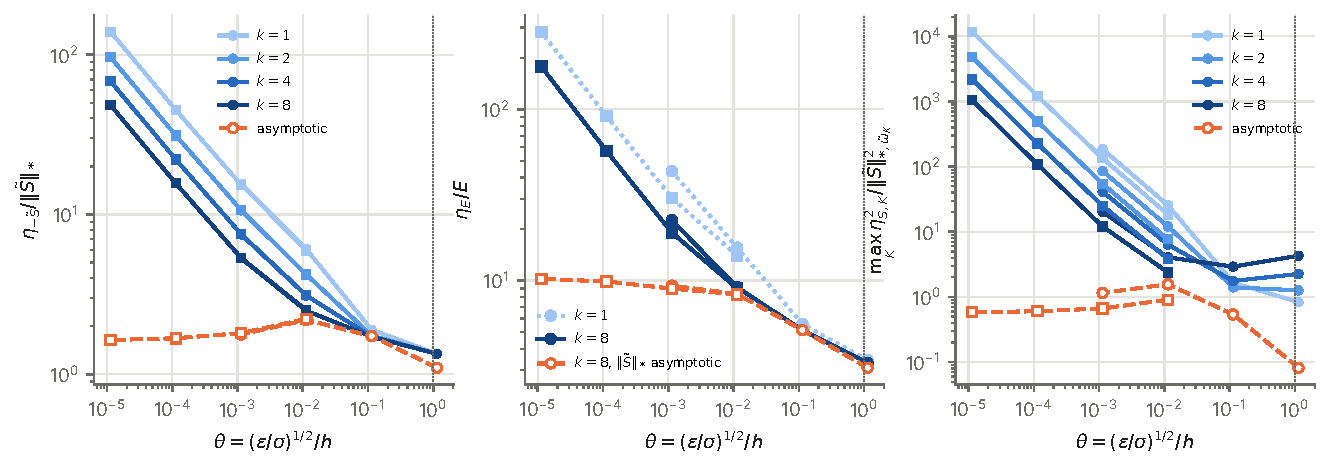
\includegraphics[width=\textwidth]{figures/sv_refref.pdf}
\caption{\asref{Reaction regime, layers problem, $n=16$, A+S estimator; circles $\sigma=1$, squares $\sigma=10^4$.
Left: $\eta_{-\Stil}/\|\Stil\|_*$ with $P_2$ references on $k$-times refined meshes and with the asymptotic value
\eqref{eq:Sasym}. Middle: $\eta_E/E$ with the same-mesh and the $8$ times refined references, and with
$\|\Stil\|_*$ from \eqref{eq:Sasym}. Right: the local ratio for $\ell=-\Stil$; the refined references are lower bounds
of the local dual norms, so these ratios are upper estimates; the asymptotic value is valid only for $\theta\ll1$.}}
\label{fig:refref}
\end{figure}

\begin{figure}[!htbp]
\centering
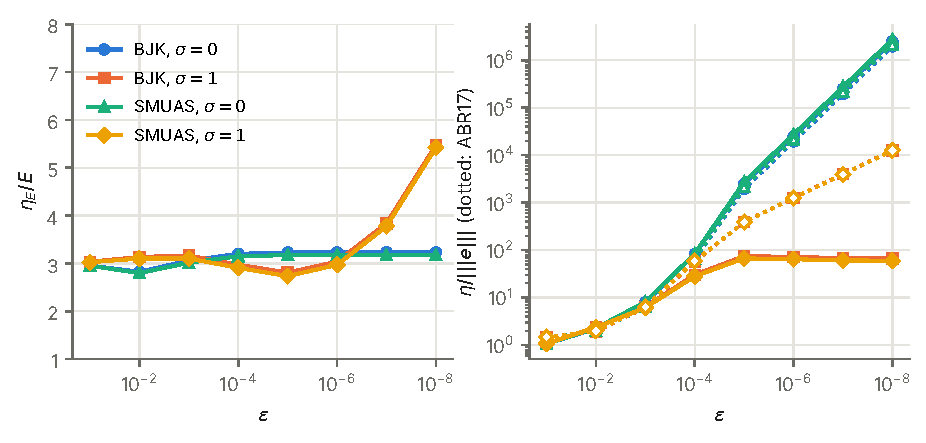
\includegraphics[width=\textwidth]{figures/sv_sweep.pdf}
\caption{Layers problem, $n=32$, as functions of $\eps$. Left: $I_E=\eta_E/E$. Right: the energy-norm
indices $\eta/\tnorm{e}$ (solid) and, dotted with open markers, that of the guaranteed bound of
\cite{ABR17}.}
\label{fig:sweep}
\end{figure}

\subsection{Variable reaction}\label{sec:num-cb}

With $c=1+(c_{\max}-1)xy$ and $\sigma=1$, the constant of (H3) is $\|c\|_\infty/\sigma=c_{\max}$, attained at
the vertex $(1,1)$. \refe{The computed $c_b$ is the sampled enclosure of Remark~\ref{rem:CF}, which is diagnostic: $c$ is not
affine on the cells, so the sampled maximum is enlarged by $\frac{h_K}2\max|\nabla c|$; here this gives} $c_b=1.12\,c_{\max}$, $1.06\,c_{\max}$
and $1.03\,c_{\max}$ for $n=8,16,32$, and $\kappa=2+c_b$ (Table~\ref{tab:cb}). The bound $E\le\eta_E$ holds in
all runs. The index of $\eta_{E,c}$ grows at most linearly, $\eta_{E,c}/E_c\le3\,c_b$ in all runs, as
Corollary~\ref{cor:twoc} predicts; it is often much smaller, down to $0.05\,c_b$, because the factor $M=c_b$ in front of $\tnorm{e}$ in $E_c$ also enlarges the
error measure. The index of $\eta_E$ grows faster, up to $5.2\,c_b$ at $c_b\approx10^3$, but stays far
below the worst case $(1+c_b)^2$ of Corollary~\ref{cor:two}. A variable reaction with a small lower
bound $\sigma$ is therefore the one situation in which the estimator loses its robustness, in
accordance with the theory; Section~\ref{sec:concl} discusses how to remove it.

% generated by examples/convection_diffusion/sv_numerics/make_figures.py; do not edit
\begin{table}[!htbp]
\centering
\small
\setlength{\tabcolsep}{4pt}
\caption{Variable reaction $c=1+(c_{\max}-1)xy$, $\sigma=1$, $\eps\in\{10^{-3},10^{-6}\}$, $n\in\{8,16,32\}$: ranges over the six runs; $c_b$ and $\kappa$ are the means of the sampled enclosures (Remark~\ref{rem:CF}; diagnostic), which exceed $c_{\max}$ by $3$--$12\,\%$.}\label{tab:cb}
\begin{tabular}{rrrllll}
\toprule
$c_{\max}$ & $c_b$ & $\kappa$ & $\eta_E/E$ & $\eta_{E,c}/E_c$ & $\eta_{E,c}/(c_bE_c)$ & $E\le\eta_E$\\
\midrule
1 & 1.00 & 3.00 & 3.85--5.34 & 3.85--5.34 & 3.85--5.34 & yes\\
10 & 10.66 & 12.66 & 14.63--19.94 & 8.69--30.35 & 0.85--2.95 & yes\\
100 & 107.22 & 109.22 & 128--271 & 12.27--216 & 0.12--2.09 & yes\\
1000 & $1.1\cdot10^{3}$ & $1.1\cdot10^{3}$ & 1618--5312 & 56.23--1125 & 0.05--1.09 & yes\\
\bottomrule
\end{tabular}
\end{table}


\subsection{Local efficiency}\label{sec:num-loc}

Table~\ref{tab:loc} reports the localised measure for the layers problem on the $16\times16$ mesh. The
local ratio $\max_K\eta_K^2/E_{\mathrm{loc}}(\tilde\omega_K)^2$ is at most $0.51$ in all cases, and
independent of $\eps$ for $\eps\le10^{-4}$: the estimator is locally efficient, as stated in
Theorem~\ref{thm:loc}. The ratio $E_{\mathrm{loc}}/E$ lies between $0.48$ and $1.01$, so on these
problems the localised measure captures most of the global one, and the guaranteed bound
$E_{\mathrm{loc}}\le\sqrt{d+1}\,\eta_E$ of Theorem~\ref{thm:loc} overestimates $E_{\mathrm{loc}}$ by a
factor $5$--$12$. The largest value, $\eta_E/E_{\mathrm{loc}}=7.0$ for $\sigma=1$ and $\eps=10^{-8}$, is the
same reference effect as in Section~\ref{sec:num-robust}.

% generated by examples/convection_diffusion/sv_numerics/make_figures.py; do not edit
\begin{table}[!htbp]
\centering
\small
\setlength{\tabcolsep}{4pt}
\caption{Localised measure (Theorem~\ref{thm:loc}), outflow layers, BJK, $n=16$. The last but one column is $\max_K\eta_K^2/E_{\mathrm{loc}}(\tilde\omega_K)^2$ with $\eta_K=\eta_{A,K}+\eta_{S,K}$.}\label{tab:loc}
\begin{tabular}{rrrrrrr}
\toprule
$\sigma$ & $\eps$ & $E_{\mathrm{loc}}/E$ & $\eta_E/E_{\mathrm{loc}}$ & $\sqrt{d+1}\,\eta_E/E_{\mathrm{loc}}$ & local max & $I_E$\\
\midrule
0 & $10^{-2}$ & 0.48 & 5.94 & 10.29 & 0.26 & 2.88\\
0 & $10^{-4}$ & 0.60 & 5.50 & 9.53 & 0.37 & 3.28\\
0 & $10^{-6}$ & 0.60 & 5.50 & 9.52 & 0.37 & 3.29\\
0 & $10^{-8}$ & 0.60 & 5.50 & 9.52 & 0.37 & 3.29\\
1 & $10^{-2}$ & 0.52 & 6.38 & 11.05 & 0.51 & 3.33\\
1 & $10^{-4}$ & 0.95 & 3.07 & 5.32 & 0.13 & 2.93\\
1 & $10^{-6}$ & 1.01 & 3.47 & 6.01 & 0.07 & 3.51\\
1 & $10^{-8}$ & 1.01 & 7.04 & 12.20 & 0.07 & 7.13\\
\bottomrule
\end{tabular}
\end{table}


\subsection{Adaptive refinement}\label{sec:num-adapt}

Starting from the $8\times8$ mesh, we mark by the indicators $\eta_K=\eta_{A,K}+\eta_{S,K}$ with the
dual strategy of \cite{AJ27} (all cells with $\eta_K\ge\theta\max\eta$, $\theta=0.5$, reduced until at least
$5\,\%$ of the cells are marked) and refine by red--green refinement, until $N>3\cdot10^4$.
Table~\ref{tab:adapt} and Figures~\ref{fig:adapt} and~\ref{fig:adaptmesh} show the results for the layers
problem.
\begin{itemize}
  \item \textbf{Effectivity.} $I_E$ stays between $2.86$ and $3.55$ in every loop of all three runs, from
  $N=81$ to $N=45\,094$, while the local mesh size spans three orders of magnitude.
  \item \textbf{Where the mesh is refined.} The refinement concentrates in the outflow layers at $x=1$ and
  $y=1$ (Figure~\ref{fig:adaptmesh}); the smallest cells have $h_{\min}=3.5\cdot10^{-4}$ for $\eps=10^{-3}$,
  below $\eps$, so the layers are resolved, and $h_{\min}=1.7\cdot10^{-4}$ for $\eps=10^{-5}$, where they are not.
  \item \textbf{Convergence.} For $\eps=10^{-3}$, $E$ decreases at the rate $1.8$--$1.9$ with respect to
  $N^{-1/2}$ over the second half of the loops: this is the pre-asymptotic phase in which the layers become
  resolved, faster than the optimal rate $1$. For $\eps=10^{-5}$ the rate is $0.98$. On the finest uniform mesh
  ($N=16\,641$) the error $E$ is $18$, $4.4$ and $17$ times larger than the adaptive error at the same $N$.
  Under uniform refinement $E$ decreases at the rate $0.46$--$0.60$ for $\sigma=0$ and $0.04$--$0.51$ for
  $\sigma=1$, because the layers are never resolved; the index $I_E$ is $2.86$--$3.37$ there as well.
  \item \textbf{Energy norm.} Along the adaptive runs the energy-norm index $I$ falls from $29$ to $1.1$
  ($\eps=10^{-3}$) and from $8.4\cdot10^3$ to $6.2$ ($\eps=10^{-5}$): once the mesh resolves the layers, the
  energy error and the dual norm of the residual become comparable, while $I_E$ is insensitive to this.
\end{itemize}

% generated by examples/convection_diffusion/sv_numerics/make_figures.py; do not edit
\begin{table}[!htbp]
\centering
\small
\setlength{\tabcolsep}{4pt}
\caption{Adaptive refinement for the outflow-layers problem, BJK, dual marking by the SV indicators $\eta_K$, red--green refinement. The rate is that of $E$ with respect to $N^{-1/2}$ over the second half of the loops; the last column is the ratio of $E$ on the finest uniform mesh ($N=16641$) to the adaptive $E$ at the same $N$.}\label{tab:adapt}
\begin{tabular}{rrrrllrlr}
\toprule
$\eps$ & $\sigma$ & loops & $N$ (last) & $h_{\min}$ & $E$ (last) & rate & $\eta_E/E$ & gain\\
\midrule
$10^{-3}$ & 0 & 15 & 33010 & $3.45\cdot10^{-4}$ & $7.395\cdot10^{-2}$ & 1.88 & 2.86--3.25 & 18.3\\
$10^{-5}$ & 0 & 12 & 31866 & $1.73\cdot10^{-4}$ & $3.941$ & 0.98 & 2.94--3.35 & 4.4\\
$10^{-3}$ & 1 & 17 & 45094 & $1.73\cdot10^{-4}$ & $5.891\cdot10^{-2}$ & 1.83 & 2.96--3.55 & 17.2\\
\bottomrule
\end{tabular}
\end{table}


\begin{figure}[!htbp]
\centering
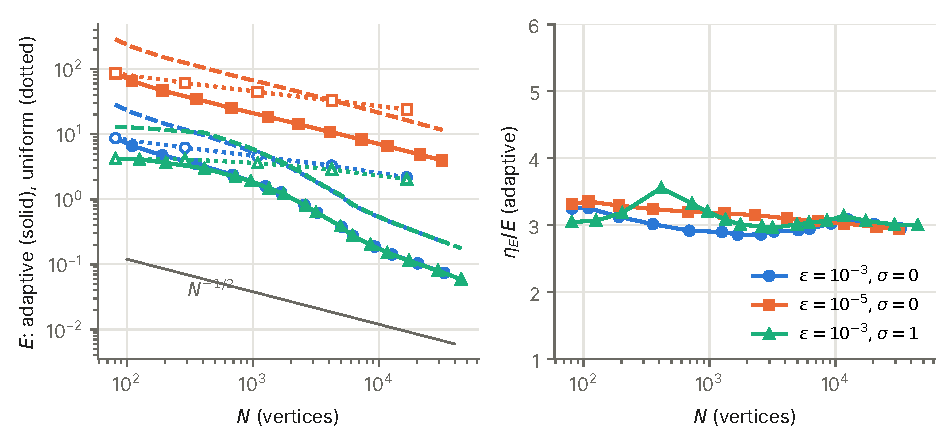
\includegraphics[width=\textwidth]{figures/sv_adapt.pdf}
\caption{Adaptive refinement, layers problem, BJK. Left: $E$ for adaptive (solid) and uniform (dotted, open
markers) refinement, and $\eta_E$ for the adaptive runs (dashed). Right: $I_E$ along the adaptive runs.}
\label{fig:adapt}
\end{figure}

\begin{figure}[!htbp]
\centering
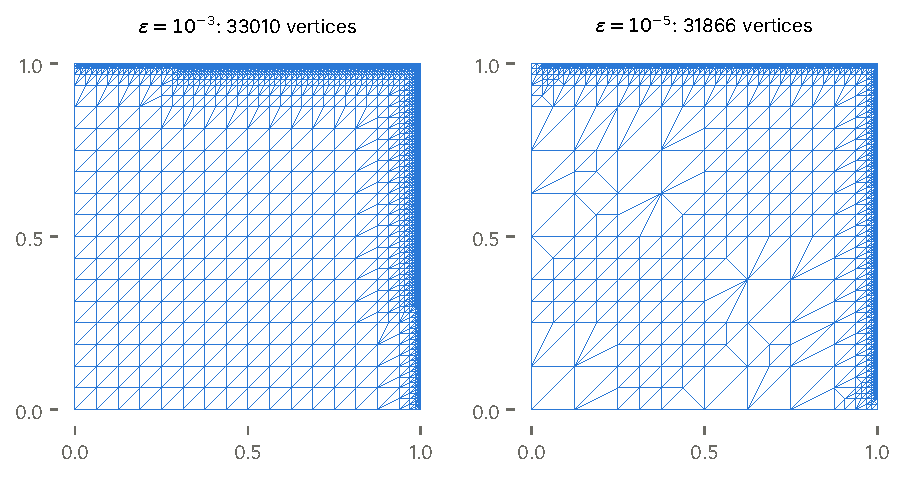
\includegraphics[width=\textwidth]{figures/sv_adapt_mesh.pdf}
\caption{Final adaptive meshes, layers problem, $\sigma=0$.}
\label{fig:adaptmesh}
\end{figure}

\subsection{\adapt{Uniform versus adaptive refinement}}\label{sec:num-unad}
{\color{magenta}

We repeat the uniform-mesh studies of Tables~\ref{tab:conv} and~\ref{tab:sweep} with adaptive refinement:
the same problems, the same marking as in Section~\ref{sec:num-adapt}, from the $8\times8$ mesh up to
$N\approx2\cdot10^4$ (Table~\ref{tab:conv}) and $N\approx10^4$ (Table~\ref{tab:sweep}). For the robustness
sweep we compare at equal cost: the adaptive loop whose $N$ is closest to $N=1089$, the size of the $32\times32$
mesh of Table~\ref{tab:sweep}.

\paragraph{Refinement studies (Figure~\ref{fig:aconv}).}
\begin{itemize}
  \item \textbf{Effectivity.} Along the adaptive runs $I_E$ lies in $2.83$--$4.18$ and tends to the same values
  as on uniform meshes, about $3.0$--$3.2$. The bound held in every loop.
  \item \textbf{Accuracy.} For the smooth solution, adaptive refinement gains nothing: at $N=16\,641$ the two
  errors agree to within $1\,\%$, and $E$ converges at the rate $1$ in both cases. For the layers problem the
  uniform error is $5.4$ ($\eps=10^{-2}$) and $5.9$ ($\eps=10^{-4}$) times the adaptive one at the same $N$.
  For $\eps=10^{-4}$, $E$ converges at the rate $0.47$ under uniform refinement and at $1.4$--$1.9$ in the last
  adaptive loops, in which the layers become resolved.
\end{itemize}

\begin{figure}[!htbp]
\centering
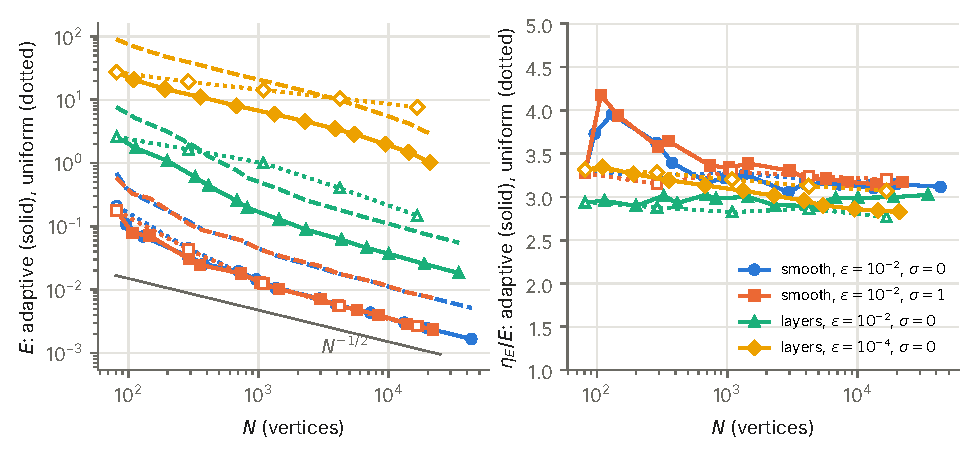
\includegraphics[width=\textwidth]{figures/sv_aconv.pdf}
\caption{\adapt{The cases of Table~\ref{tab:conv} under adaptive refinement. Left: $E$ for adaptive (solid) and uniform
(dotted, open markers) refinement, and $\eta_E$ for the adaptive runs (dashed). Right: $I_E$, adaptive (solid) and
uniform (dotted).}}
\label{fig:aconv}
\end{figure}

\paragraph{Robustness sweep (Figures~\ref{fig:abudget} and~\ref{fig:aloops}).}
\begin{itemize}
  \item \textbf{$\sigma=0$.} At equal cost, $I_E=2.89$--$3.22$ on the adaptive meshes against $2.80$--$3.23$ on the
  uniform mesh, for all $\eps$ and both stabilisations, and it stays in $2.82$--$3.35$ over all loops: the
  estimator is as robust on the meshes it generates as on the fixed mesh.
  \item \textbf{$\sigma=1$, small $\eps$.} The rise of $I_E$ to $5.4$--$5.5$ on the uniform mesh at
  $\eps\le10^{-7}$ (Section~\ref{sec:num-robust}) does not occur at equal cost on the adaptive meshes, where
  $I_E=2.75$--$3.16$. Figure~\ref{fig:aloops} shows why. The large values, up to $9.6$, appear only on the
  coarse initial mesh, and they come from the stabilisation part: $I_S=17.8$ at $N=81$ for $\eps=10^{-8}$. As the
  mesh resolves the layers, $I_S$ falls to $1.5$--$1.6$ and $I_E$ returns to about $3$. This confirms that the
  rise on the uniform mesh is a property of the under-resolved $P_2$ reference for $\|\Stil\|_*$, not of the
  estimator.
  \item \textbf{Smooth problem.} For $\eps\le10^{-3}$ the adaptive indices are higher than the uniform ones at
  equal cost: $I_E=4.0$--$5.3$ against $3.6$--$3.8$ for $\sigma=0$, and $4.5$--$6.0$ against $3.9$--$6.0$ for
  $\sigma=1$. Along the runs they reach $7.8$ after the first loop, and $10.9$ on the initial mesh. For $\sigma=1$
  and $\eps\le10^{-6}$ the fixed-point iteration reaches the iteration limit $2\cdot10^4$ on most meshes beyond
  $N\approx1100$, and the bound holds at these iterates.
  \item \textbf{Energy norm.} At $\sigma=0$ the energy-norm index still grows like $\eps^{-1}$ on the adaptive meshes,
  to $4\cdot10^5$ at $\eps=10^{-8}$ (uniform: $2.5\cdot10^6$); only the augmented measure is robust.
  \item \textbf{An open point.} For the layers problem with $\sigma=1$ and $\eps=10^{-6}$, $I_E$ rises again in the
  last loops, from $2.8$ to $4.3$, together with $I_\oplus$ (from $3.2$ to $6.6$). We have not identified the cause;
  it may be the convective part of the reference becoming resolved, and would need runs beyond $N=10^4$.
\end{itemize}

\begin{figure}[!htbp]
\centering
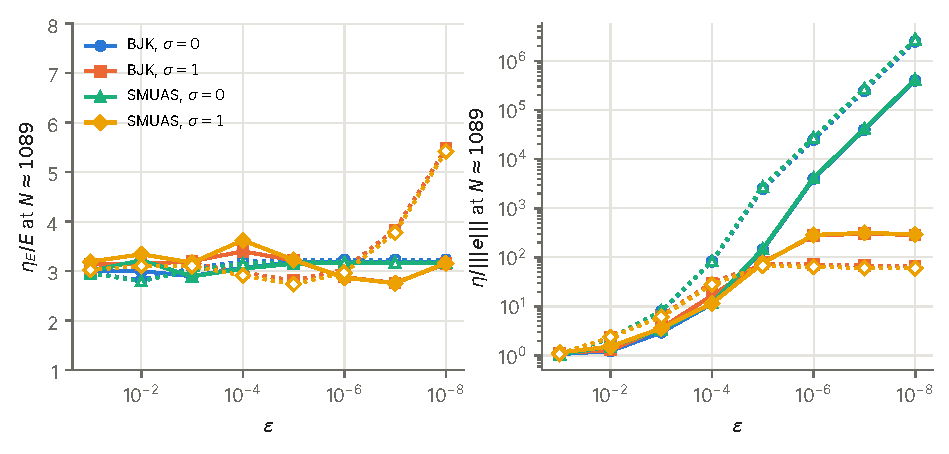
\includegraphics[width=\textwidth]{figures/sv_asweep_budget.pdf}
\caption{\adapt{The robustness sweep of Table~\ref{tab:sweep} at equal cost, layers problem: adaptive meshes with
$N\approx1089$ (solid) against the uniform $32\times32$ mesh (dotted, open markers). Left: $I_E$. Right: the
energy-norm index $\eta/\tnorm{e}$.}}
\label{fig:abudget}
\end{figure}

\begin{figure}[!htbp]
\centering
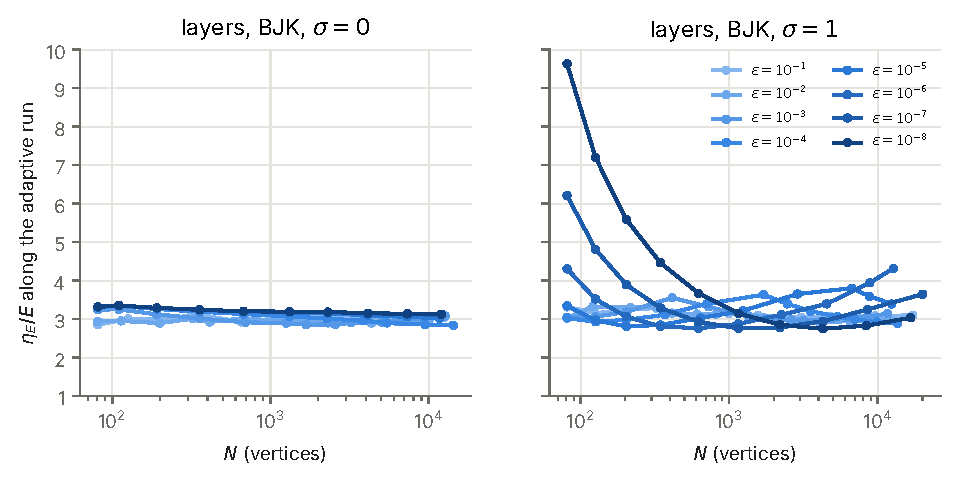
\includegraphics[width=\textwidth]{figures/sv_asweep_loops.pdf}
\caption{\adapt{$I_E$ along the adaptive runs of the robustness sweep, layers problem, BJK; one line per $\eps$, darker for
smaller $\eps$.}}
\label{fig:aloops}
\end{figure}

\paragraph{Which refinement to use.} For computing solutions, adaptive refinement is clearly preferable when the
solution has layers, by factors $4$--$18$ in $E$ at equal $N$, and it is what the estimator is designed for. For
testing the theory, the uniform meshes remain the primary evidence: a fixed coarse mesh keeps the layers
unresolved, which is the regime in which robustness can fail, isolates the dependence on $\eps$ and $\sigma$, and
is the only setting in which rates in $h$ are meaningful. The adaptive runs confirm that the effectivity stays at
about $3$ on the meshes the estimator generates itself.
}% end of the magenta block

\subsection{Inexact iterates and adaptive stopping}\label{sec:num-stop}

\paragraph{Iterates.} Table~\ref{tab:iter} and Figure~\ref{fig:iter} evaluate the estimator at the
fixed-point iterates $u^i$ on the $16\times16$ mesh. The index $I_E$ stays between $2.9$ and $5.3$ at
every iterate, including the first one, where the algebraic part $\eta_{\mathrm{alg}}$ is up to $71\,\%$
of $\eta_{\mathrm{disc}}$: this is part~2 of Proposition~\ref{prop:stop}, efficiency at every iterate
without any condition on the algebraic error. The ratio $\eta_{\mathrm{alg}}/\eta_{\mathrm{disc}}$
decreases monotonically for all problems except the smooth one with $\eps=10^{-6}$ and $\sigma=0$, for
which the fixed-point iteration does not converge in $2\cdot10^4$ iterations; there the ratio stalls
between $10^{-3}$ and $4\cdot10^{-3}$. In that case the error is smallest at $i\approx10$, $E(u^{10})=4.8$, and grows to
$8.4$ at $i=2\cdot10^4$: further iterations make the iterate worse in $E$, and the estimator, which is
efficient at every iterate, reflects this.

% generated by examples/convection_diffusion/sv_numerics/make_figures.py; do not edit
\begin{table}[!htbp]
\centering
\small
\setlength{\tabcolsep}{4pt}
\caption{Fixed-point iterates $u^i$, $i\in\{1,2,5,\dots,1000\}$ below the converged count, and the converged solution; BJK, $n=16$. The split is $\eta_{\mathrm{disc}}=\eta_E-\eta_{\mathrm{alg}}$.}\label{tab:iter}
\begin{tabular}{lrrrlrrl}
\toprule
problem & $\eps$ & $\sigma$ & it.\ to tol. & $\eta_E/E$ over $i$ & $\max_i\eta_{\mathrm{alg}}/\eta_{\mathrm{disc}}$ & $E(u^1)/E(u^{\mathrm{last}})$ & $E\le\eta_E$\\
\midrule
smooth & $10^{-2}$ & 0 & 39 & 3.24--3.63 & 0.71 & 1.81 & yes\\
smooth & $10^{-2}$ & 1 & 37 & 3.15--3.45 & 0.51 & 1.58 & yes\\
smooth & $10^{-6}$ & 0 & 20000 & 3.76--4.61 & 0.58 & 1.06 & yes\\
smooth & $10^{-6}$ & 1 & 664 & 4.42--5.28 & 0.19 & 1.20 & yes\\
layers & $10^{-2}$ & 0 & 47 & 2.88--2.97 & 0.02 & 1.01 & yes\\
layers & $10^{-2}$ & 1 & 45 & 3.32--3.33 & 0.01 & 1.01 & yes\\
layers & $10^{-6}$ & 0 & 635 & 3.29--3.47 & 0.04 & 1.01 & yes\\
layers & $10^{-6}$ & 1 & 502 & 3.51--3.56 & 0.02 & 1.03 & yes\\
\bottomrule
\end{tabular}
\end{table}


\begin{figure}[!htbp]
\centering
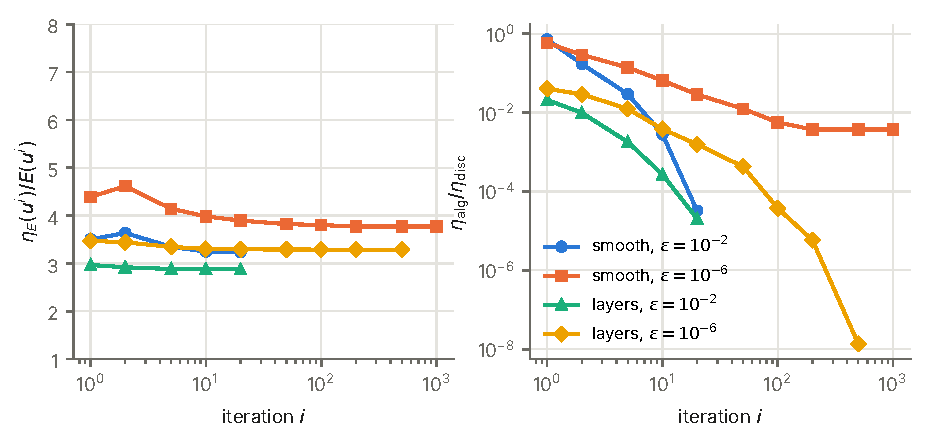
\includegraphics[width=\textwidth]{figures/sv_iter.pdf}
\caption{Fixed-point iterates, BJK, $\sigma=0$, $n=16$. Left: $I_E$ at the iterate $u^i$. Right: the
ratio $\eta_{\mathrm{alg}}/\eta_{\mathrm{disc}}$ (points with a ratio below $10^{-8}$ are omitted).}
\label{fig:iter}
\end{figure}

\paragraph{Adaptive stopping.} Table~\ref{tab:stop} runs five adaptive loops \refe{as in} Section~\ref{sec:num-adapt}
in which the fixed-point iteration is stopped either at the fixed tolerance $\|r\|\le10^{-10}\sqrt N$ or by
the criterion \eqref{eq:stop}, $\eta_{\mathrm{alg}}\le\gamma\eta_{\mathrm{disc}}$, with
$\eta_{\mathrm{disc}}=\eta_E-\eta_{\mathrm{alg}}$; each loop starts from the zero initial guess.
\begin{itemize}
  \item \textbf{Savings.} With $\gamma=0.1$, the total number of iterations drops from $227$ to $25$ (smooth,
  $\eps=10^{-2}$) and from $2323$ to $25$ (layers, $\eps=10^{-4}$), by factors $9$ and $93$; with $\gamma=0.01$
  the factors are $4.5$ and $46$.
  \item \textbf{Accuracy.} The final error $E$ changes by at most $6\,\%$ ($\gamma=0.1$, layers) and by at most
  $0.3\,\%$ for $\gamma\le0.01$. The index $I_E$ stays in $3.1$--$4.8$ in all runs, and in every stopped loop
  $\eta_{\mathrm{alg}}/\eta_{\mathrm{disc}}\le\gamma$, so $E\le(1+\gamma)\eta_{\mathrm{disc}}$
  (Proposition~\ref{prop:stop}, part~3).
  \item \textbf{Non-converging iteration.} For the smooth problem with $\eps=10^{-6}$ the fixed-point
  iteration does not reach the tolerance within $10^4$ iterations on any mesh, and $50\,000$ iterations give
  $E=3.22$. The criterion with $\gamma=0.1$ stops after $5$--$15$ iterations per loop, $50$ in total, with a
  \emph{smaller} error, $E=1.98$: as in Figure~\ref{fig:iter}, the early iterates are better than the late
  ones. For $\gamma=10^{-3}$ the criterion fires in only one of the five loops, since $\eta_{\mathrm{alg}}/\eta_{\mathrm{disc}}$ stalls
  at about $3\cdot10^{-3}$; this is a property of the iteration, not of the estimator.
\end{itemize}

% generated by examples/convection_diffusion/sv_numerics/make_figures.py; do not edit
\begin{table}[!htbp]
\centering
\footnotesize
\setlength{\tabcolsep}{4pt}
\caption{Adaptive stopping in five adaptive loops (dual marking by the SV indicators, red--green refinement), BJK, $\sigma=0$. ``tol.'' is the fixed tolerance $\|r\|\le10^{-10}\sqrt N$; otherwise the iteration stops at $\eta_{\mathrm{alg}}\le\gamma\eta_{\mathrm{disc}}$ (at most $10^4$ iterations). The last column says whether every loop stopped before the iteration limit.}\label{tab:stop}
\begin{tabular}{lrrrrlllr}
\toprule
problem & $\eps$ & $\gamma$ & it./loop & total & $E$ (last) & $\eta_E/E$ & $\max\eta_{\mathrm{alg}}/\eta_{\mathrm{disc}}$ & stopped\\
\midrule
smooth & $10^{-2}$ & tol. & 30--59 & 227 & $2.550\cdot10^{-2}$ & 3.29--3.95 & $5.78\cdot10^{-8}$ & yes\\
smooth & $10^{-2}$ & 0.1 & 5 & 25 & $2.554\cdot10^{-2}$ & 3.41--3.97 & $5.07\cdot10^{-2}$ & yes\\
smooth & $10^{-2}$ & 0.01 & 10 & 50 & $2.551\cdot10^{-2}$ & 3.33--3.98 & $7.27\cdot10^{-3}$ & yes\\
smooth & $10^{-2}$ & 0.001 & 10--20 & 80 & $2.551\cdot10^{-2}$ & 3.29--3.96 & $9.89\cdot10^{-4}$ & yes\\
smooth & $10^{-6}$ & tol. & 10000 & 50000 & $3.218$ & 3.77--4.58 & $3.03\cdot10^{-3}$ & no\\
smooth & $10^{-6}$ & 0.1 & 5--15 & 50 & $1.984$ & 4.04--4.79 & $9.83\cdot10^{-2}$ & yes\\
smooth & $10^{-6}$ & 0.01 & 120--760 & 2190 & $2.749$ & 3.80--4.45 & $9.10\cdot10^{-3}$ & yes\\
smooth & $10^{-6}$ & 0.001 & 7320--10000 & 47320 & $3.218$ & 3.77--4.58 & $3.03\cdot10^{-3}$ & no\\
layers & $10^{-4}$ & tol. & 385--628 & 2323 & $8.044$ & 3.13--3.34 & $3.57\cdot10^{-9}$ & yes\\
layers & $10^{-4}$ & 0.1 & 5 & 25 & $8.524$ & 3.20--3.42 & $2.49\cdot10^{-2}$ & yes\\
layers & $10^{-4}$ & 0.01 & 10 & 50 & $8.023$ & 3.15--3.38 & $8.43\cdot10^{-3}$ & yes\\
layers & $10^{-4}$ & 0.001 & 25--50 & 175 & $8.04$ & 3.14--3.35 & $9.29\cdot10^{-4}$ & yes\\
\bottomrule
\end{tabular}
\end{table}


\subsection{Variable diffusion}\label{sec:num-vareps}

Table~\ref{tab:vareps} reports the variable-diffusion problems on the meshes $n=8,16,32$. All bounds are
guaranteed. For the smooth coefficient, the oscillation $\eta_\eps$ converges at the rate $2.09$--$2.13$
in $h$, in accordance with Lemma~\ref{lem:V}(iii), and is at most $12\,\%$ of $\eta$ (at contrast $10^4$ on
the coarsest mesh). For the jump aligned with the mesh, $\Pi_1\eps=\eps$ and $\eta_\eps=0$. The
effectivity $I_E$ lies in $2.6$--$4.5$ for contrasts up to $10^4$, for $\eps=10^{-2}$ and $10^{-6}$ alike. For
the jump it does not grow with the contrast; for the smooth coefficient it grows mildly, from
$3.1$ at contrast $1$ to at most $4.3$ at contrast $10^4$ (on the coarsest mesh). This is the quasi-monotone case; the constants of
Theorem~\ref{thm:vareps} depend on the patch contrast, but for an aligned jump that contrast does not
show up in the indices. Checkerboard (non-quasi-monotone) coefficients are not tested; for them no
local estimator can be robust \cite{Li26}.

% generated by examples/convection_diffusion/sv_numerics/make_figures.py; do not edit
\begin{table}[!htbp]
\centering
\footnotesize
\setlength{\tabcolsep}{4pt}
\caption{Variable diffusion, BJK, $\sigma=0$, $n\in\{8,16,32\}$: ranges over the three meshes. The rate is that of $\eta_\eps$ with respect to $N^{-1/2}$ between $n=16$ and $n=32$ (expected: $2$).}\label{tab:vareps}
\begin{tabular}{lrrllllrl}
\toprule
$\eps(x)$ & $\eps$ & contrast & $I$ & $I_\oplus$ & $I_E$ & $\max\eta_\eps/\eta$ & rate & $E\le\eta_E$\\
\midrule
smooth & $10^{-2}$ & 1 & 1.23--4.58 & 3.30--4.06 & 3.07--3.13 & 0.000 & --- & yes\\
smooth & $10^{-2}$ & 100 & 1.07--1.24 & 3.16--3.39 & 3.15--3.26 & 0.035 & 2.09 & yes\\
smooth & $10^{-2}$ & 10000 & 1.10--1.44 & 3.30--4.28 & 3.29--4.27 & 0.117 & 2.09 & yes\\
smooth & $10^{-6}$ & 1 & 7959--36796 & 3.72--5.01 & 3.50--3.70 & 0.000 & --- & yes\\
smooth & $10^{-6}$ & 100 & 818--3354 & 3.73--5.44 & 3.54--4.03 & 0.000 & 2.13 & yes\\
smooth & $10^{-6}$ & 10000 & 64.07--336 & 4.31--5.49 & 3.94--4.46 & 0.001 & 2.10 & yes\\
jump & $10^{-2}$ & 100 & 2.56--7.63 & 3.43--4.18 & 2.61--2.99 & 0.000 & --- & yes\\
jump & $10^{-2}$ & 10000 & 2.61--8.12 & 3.43--4.22 & 2.60--3.01 & 0.000 & --- & yes\\
jump & $10^{-6}$ & 100 & 9025--28125 & 4.75--5.12 & 3.44--3.54 & 0.000 & --- & yes\\
jump & $10^{-6}$ & 10000 & 2156--4989 & 4.78--5.08 & 3.41--3.52 & 0.000 & --- & yes\\
\bottomrule
\end{tabular}
\end{table}


\subsection{Three dimensions}\label{sec:num-3d}

Table~\ref{tab:d3} repeats the uniform-refinement study on the unit cube ($n=4,8,16$, up to $N=4913$
vertices and $24\,576$ tetrahedra).
\begin{itemize}
  \item \textbf{Layers.} $I_E=2.94$--$3.55$ for $\eps=10^{-2}$ and $10^{-6}$, as in two dimensions; $I_\oplus\le4.9$
  and $I_S=1.21$--$1.26$.
  \item \textbf{Smooth solution.} $I_E$ is higher than in two dimensions, $5.1$--$6.4$, but decreases under
  refinement for both values of $\eps$ ($5.97\to5.40$ and $6.39\to5.09$). These meshes are coarse: $E$ still
  converges at the pre-asymptotic rates $2.1$--$2.7$ in $h$, dominated by the stabilisation part
  $\|\Stil\|_*$, which is estimated sharply ($I_S=1.28$--$1.31$); the larger index comes from the convective
  dual norm on coarse tetrahedral meshes. For $\eps=10^{-6}$ on the finest mesh the fixed-point iteration does
  not converge within $2\cdot10^4$ iterations, and the bound still holds at the last iterate.
  \item \textbf{Energy norm.} As in two dimensions, $I$ is useless for $\sigma=0$ and small $\eps$
  ($1.0\cdot10^4$--$1.4\cdot10^5$ at $\eps=10^{-6}$, against $2.6$--$9.3$ at $\eps=10^{-2}$), while $I_E$ is not
  affected.
  \item \textbf{Cost.} The estimator takes about $8$\,s at $N=729$ and $220$--$240$\,s at $N=4913$ in our
  Python implementation; the cost is dominated by the vertex-patch problems in $\RTN$, whose size grows
  quickly with the number of tetrahedra per patch in three dimensions. The patch problems are independent and
  can be solved in parallel; the global $\RT_0$ defect problem takes a small fraction of the time.
\end{itemize}

% generated by examples/convection_diffusion/sv_numerics/make_figures.py; do not edit
\begin{table}[!htbp]
\centering
\small
\setlength{\tabcolsep}{4pt}
\caption{Three dimensions, uniform refinement of the unit cube, BJK, $\sigma=0$. Rates with respect to $N^{-1/3}\sim h$; the last column is the time of the estimator in seconds.}\label{tab:d3}
\begin{tabular}{lrrlrrrrr}
\toprule
problem & $\eps$ & $N$ & $E$ & rate & $I$ & $I_\oplus$ & $I_E$ & time\\
\midrule
smooth & $10^{-2}$ & 125 & $0.7$ &  & 9.27 & 7.82 & 5.97 & 0.7\\
smooth & $10^{-2}$ & 729 & $0.144$ & 2.69 & 4.83 & 6.98 & 5.71 & 9.0\\
smooth & $10^{-2}$ & 4913 & $3.55\cdot10^{-2}$ & 2.20 & 2.64 & 5.84 & 5.40 & 226.6\\
smooth & $10^{-6}$ & 125 & $6.72\cdot10^{1}$ &  & $7.4\cdot10^{4}$ & 9.26 & 6.39 & 0.6\\
smooth & $10^{-6}$ & 729 & $2.00\cdot10^{1}$ & 2.06 & $2.8\cdot10^{4}$ & 6.93 & 5.31 & 8.4\\
smooth & $10^{-6}$ & 4913 & $4.06$ & 2.51 & $1.0\cdot10^{4}$ & 5.56 & 5.09 & 238.0\\
layers & $10^{-2}$ & 125 & $2.74$ &  & 6.67 & 4.01 & 3.10 & 0.6\\
layers & $10^{-2}$ & 729 & $1.82$ & 0.70 & 4.31 & 3.71 & 3.01 & 8.0\\
layers & $10^{-2}$ & 4913 & $1.14$ & 0.73 & 2.93 & 3.64 & 2.94 & 217.3\\
layers & $10^{-6}$ & 125 & $2.79\cdot10^{2}$ &  & $1.4\cdot10^{5}$ & 4.71 & 3.38 & 0.5\\
layers & $10^{-6}$ & 729 & $2.01\cdot10^{2}$ & 0.56 & $7.3\cdot10^{4}$ & 4.78 & 3.47 & 8.5\\
layers & $10^{-6}$ & 4913 & $1.35\cdot10^{2}$ & 0.63 & $3.8\cdot10^{4}$ & 4.93 & 3.55 & 236.1\\
\bottomrule
\end{tabular}
\end{table}


\subsection{Summary}

The experiments answer the questions (Q1)--(Q7) as follows.
\begin{enumerate}[label=(Q\arabic*)]
  \item The bound $E\le\eta_E$ held in every run: two and three dimensions, both stabilisations,
  $\eps=10^{-1},\dots,10^{-8}$, $\sigma\in\{0,1\}$, variable reaction and diffusion, adaptive meshes and inexact
  iterates\refe{, and so did $I\ge1$, $I_\oplus\ge1$ and $I_S\ge1$. Since the references are lower bounds of the dual
  norms, this is a consistency check rather than a proof}.
  \item For constant coefficients, $I_E$ lies in $2.6$--$5.3$ in two dimensions, inexact iterates included,
  independently of $\eps$, $\sigma$, the stabilisation and the mesh; the only exception is a rise to $6.0$
  ($n=32$) and $7.1$ ($n=16$) at $\sigma=1$, $\eps\le10^{-7}$, \adapt{which the adaptive runs identify as an
  under-resolved reference for $\|\Stil\|_*$ (Section~\ref{sec:num-unad})}\asref{, as the asymptotically exact
  reference \eqref{eq:Sasym} confirms ($I_S=1.6$--$2.2$ and $\eta_E/E=8.3$--$10.2$ for $\theta$ down to $10^{-5}$)}; in three dimensions it is $2.9$--$6.4$ and
  decreases under refinement. The energy-norm index $I$, and the guaranteed bound of \cite{ABR17}, are not
  robust.
  \item The effectivity grows with $c_b$, at most linearly for $\eta_{E,c}$ and well below $c_b^2$ for $\eta_E$:
  a variable reaction with a small lower bound is the one case in which robustness is lost, as the theory
  predicts.
  \item The local ratio $\max_K\eta_K^2/E_{\mathrm{loc}}(\tilde\omega_K)^2$ is at most $0.51$.
  \item Adaptive refinement driven by $\eta_K$ resolves the layers and reduces $E$ by factors $4$--$18$
  against uniform refinement at equal $N$, with $I_E=2.9$--$3.6$ throughout. \adapt{Repeating the refinement and
  robustness studies adaptively gives the same effectivity, about $3$, as on uniform meshes.}
  \item The estimator is efficient at every iterate, and the stopping criterion saves up to $99\,\%$ of the
  iterations at a change of the error of at most $6\,\%$ ($\gamma=0.1$) or $0.3\,\%$ ($\gamma\le0.01$).
  \item For variable diffusion, $\eta_\eps$ converges at rate $2$ and $I_E$ stays in $2.6$--$4.5$ up to contrast
  $10^4$.
\end{enumerate}

\paragraph{Reproducibility.} All results are produced by the scripts \texttt{run\_numerics.py} and
\texttt{make\_figures.py} in the directory
\path{examples/convection_diffusion/sv_numerics} of \texttt{galerkit}. The first runs the experiments (about
$35$ minutes on four cores, the three-dimensional runs sequentially because of their memory use); the
second writes the tables, the figures and, for every stored solution, a VTK file
(\texttt{.vtu}) with $u_h$, $u$, $u-u_h$, $\eps$, $\eta_K$, $\tnorm{e}_K$ and the local effectivity
$\eta_K/\tnorm{e}_K$. \adapt{The figures of Section~\ref{sec:num-unad} are produced by
\texttt{make\_adaptive\_figures.py} in the same directory.}

).
% Data: examples/convection_diffusion/sv_numerics/run_numerics.py (output/*.json);
% tables and figures: make_figures.py -> tables/*.tex, figures/sv_*.{pdf,png}.
% All numbers quoted in the text below are read off those tables.

% ===========================================================================
\section{Numerical experiments}\label{sec:num}
% ===========================================================================

We test the estimator against the exact error. The questions are the ones raised by the theory:
\begin{enumerate}[label=(Q\arabic*)]
  \item Is the bound guaranteed, $E\le\eta_E$, in every run (Theorem~\ref{thm:rel})?
  \item Are the effectivity indices bounded independently of $\eps$, $\sigma$ and the stabilisation
  (Theorem~\ref{thm:eff}, Corollary~\ref{cor:two}), and do they stay bounded under refinement?
  \item Does the dependence on $c_b$ follow Corollaries~\ref{cor:two} and~\ref{cor:twoc}?
  \item Is the estimator locally efficient in the localisable measure (Theorem~\ref{thm:loc})?
  \item Do the indicators drive adaptive refinement to the optimal rate?
  \item Are the bounds valid at inexact iterates, and does the stopping criterion of
  Proposition~\ref{prop:stop} save iterations without spoiling the error?
  \item Does the variable-diffusion version keep its effectivity, with $\eta_\eps=O(h^2)$
  (Theorem~\ref{thm:vareps})?
\end{enumerate}

\subsection{Setup}

\paragraph{Discretisation.} Conforming $P_1$ elements on uniform meshes of the unit square
($n\times n$ squares, each cut into two triangles; $N=(n+1)^2$ vertices) or the unit cube ($n^3$
cubes, each cut into six tetrahedra), and on red--green refined meshes in the adaptive runs. The
stabilisations are the AFC scheme with the limiter of \cite{BJK17} (BJK), and the symmetrised
monotone upwind-type algebraic stabilisation of \cite{Kn23} (SMUAS). The nonlinear problem is solved
by the damped fixed-point iteration of \cite{AJ27} up to $\|r\|\le10^{-10}\sqrt N$, with at most
$2\cdot10^4$ iterations, unless stated otherwise.

\paragraph{Test problems} (all with $b$ constant, so $\sigma=c$, $c_b=1$ and $\kappa=3$, except in
Section~\ref{sec:num-cb}).
\begin{itemize}
  \item \emph{smooth}: $u=\prod_i\sin(\pi x_i)+x_1^2\prod_{i>1}x_i$, $b=(1,\tfrac12)$ or
  $(1,\tfrac12,\tfrac14)$, Dirichlet data on $\partial\Omega$; $f$ is computed from $u$. The solution
  has no layers, so its error is not dominated by layers, but for small $\eps$ the scheme is
  convection-dominated on every mesh used.
  \item \emph{layers}: $u=\prod_iw(x_i)$ with
  $w(s)=s-\bigl(e^{(s-1)/\eps}-e^{-1/\eps}\bigr)/\bigl(1-e^{-1/\eps}\bigr)$, $b=(1,\dots,1)$, homogeneous
  Dirichlet data; $u$ has exponential layers of width $\eps$ at the outflow boundary $x_i=1$.
  \item \emph{variable diffusion}: $u=\phi(x_1)\prod_{i>1}4x_i(1-x_i)$, either with
  $\eps(x)=\eps\,k^{x_1}$, $\phi(s)=4s(1-s)$ (\emph{smooth}), or with $\eps$ jumping from $\eps$ to $k\eps$
  at $x_1=\frac12$ and $\phi$ chosen such that the flux $\eps\phi'$ is continuous (\emph{jump}); $k$ is
  the contrast.
\end{itemize}

\paragraph{Error measures.} $\tnorm{e}$ is computed with a quadrature of degree~8. The dual norms
$\|B_A'(e,\cdot)\|_*$ and $\|\Stil\|_*$, and the local dual norms of $E_{\mathrm{loc}}$, are computed
from their Riesz representatives in the $P_2$ space on the same mesh (on each vertex patch for
$E_{\mathrm{loc}}$). These are \emph{lower} bounds of the true dual norms, so the reported effectivity
indices are slight overestimates; they become crude when the dual norm concentrates in layers that
the mesh does not resolve (see Section~\ref{sec:num-robust}). We report the effectivity indices
\[
  I=\frac{\eta}{\tnorm{e}},\qquad I_\oplus=\frac{\kappa\eta}{\tnorm{e}_\oplus},\qquad
  I_S=\frac{\eta_S}{\|\Stil\|_*},\qquad I_E=\frac{\eta_E}{E},
\]
of which $I_E$ is the one covered by Corollary~\ref{cor:two}; $I_\oplus\ge1$ and $I\ge1$ are guaranteed
too, but only $I_\oplus$ is expected to be robust.

\subsection{Solutions and indicators}

Figure~\ref{fig:snap} shows the discrete solution of the layers problem for $\eps=10^{-3}$ on the
$32\times32$ mesh, the cell indicators $\eta_K=\eta_{A,K}+\eta_{S,K}$, and the local energy errors
$\tnorm{e}_K$. The mesh does not resolve the layers ($h\approx4.4\cdot10^{-2}\gg\eps$); the AFC
solution is free of oscillations, and both the indicators and the error concentrate in the cells at
the outflow boundary, with a decay of several orders of magnitude into the interior. The indicator
is larger than $\tnorm{e}_K$ in the layer cells: it measures the residual in the dual norm, which
contains the convective part $\|B_A'(e,\cdot)\|_*$ of the error.

\begin{figure}[!htbp]
\centering
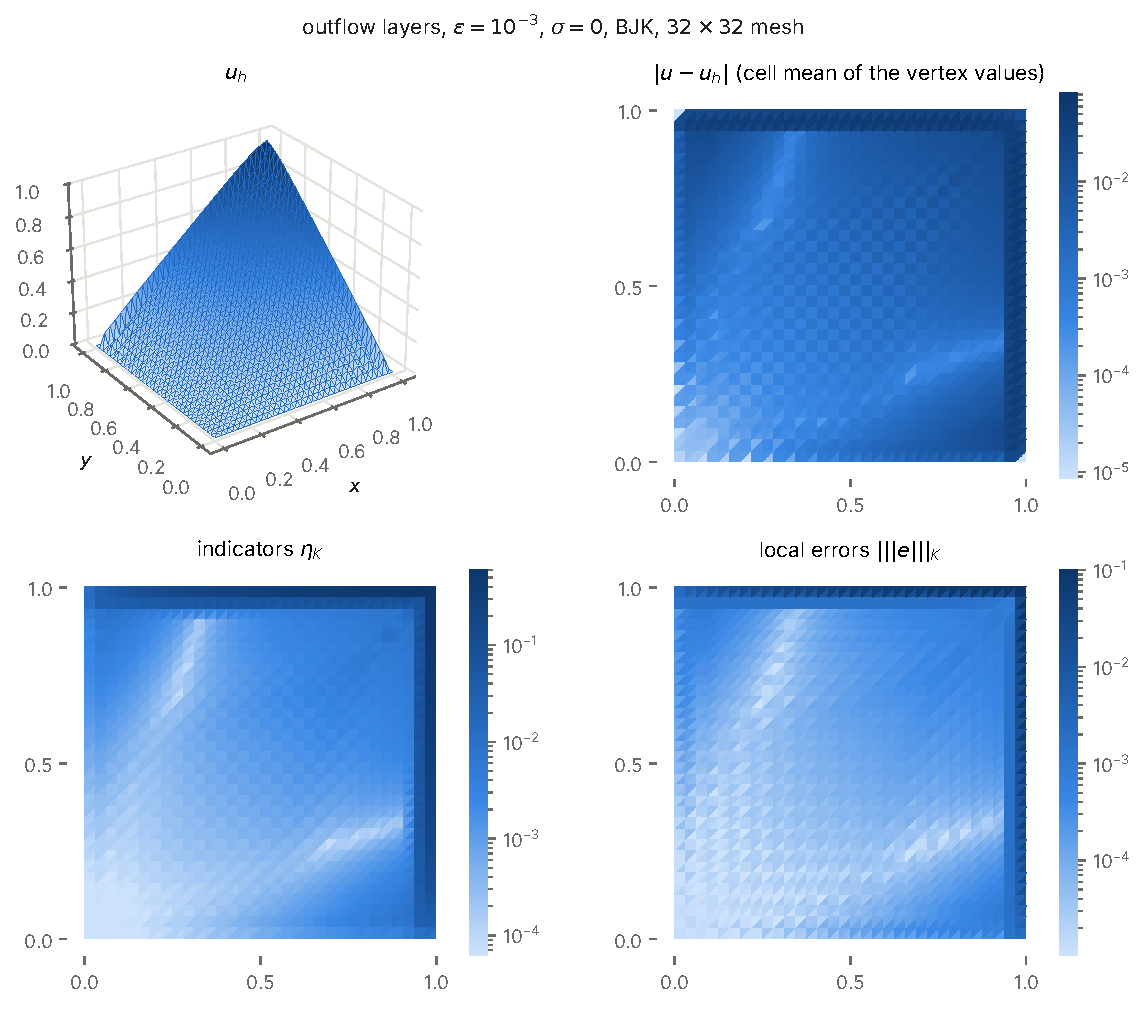
\includegraphics[width=\textwidth]{figures/sv_snap.pdf}
\caption{Layers problem, $\eps=10^{-3}$, $\sigma=0$, BJK, $n=32$: discrete solution $u_h$, indicators
$\eta_K$ and local errors $\tnorm{e}_K$ (logarithmic colour scale, common to both).}
\label{fig:snap}
\end{figure}

\subsection{Uniform refinement}\label{sec:num-conv}

Table~\ref{tab:conv} and Figure~\ref{fig:conv} report uniform refinement from $n=8$ to $n=128$.
\begin{itemize}
  \item \textbf{Smooth solution, $\eps=10^{-2}$.} $E$ and $\eta_E$ converge at the optimal rate $1$ in
  $h$ once the mesh resolves the solution; on the coarse meshes both decrease faster, because the
  stabilisation term $\|\Stil\|_*$ dominates $E$ there and decreases at a higher rate. The effectivity
  $I_E$ lies between $3.15$ and $3.29$ for $\sigma=0$ and $\sigma=1$ alike. The energy-norm index $I$
  tends to $1.1$: in the diffusion-dominated regime the energy norm and the dual norm of the
  residual coincide asymptotically.
  \item \textbf{Layers, $\eps=10^{-2}$.} The layers are resolved only from $n=64$ on, and the
  convergence of $E$ accelerates accordingly; $I_E$ stays between $2.77$ and $2.94$.
  \item \textbf{Layers, $\eps=10^{-4}$.} The meshes never resolve the layers. The energy error
  $\tnorm{e}$ \emph{increases} under refinement, because the error, concentrated in the outflow
  cells, sees an increasing part of the layer, while $E$ is dominated by the convective dual norm and
  decreases at the rate $0.45$--$0.53$; $\eta_E$ follows it with the rate $0.49$--$0.55$. The index $I_E$
  is $3.07$--$3.31$ on every mesh, whereas the energy-norm index $I$ falls from $833$ to $18.7$: the
  energy-norm bound is guaranteed but useless in this regime, which is why the error is measured in
  $E$.
\end{itemize}

% generated by examples/convection_diffusion/sv_numerics/make_figures.py; do not edit
\begin{table}[!htbp]
\centering
\small
\setlength{\tabcolsep}{4pt}
\caption{Uniform refinement in 2D, BJK. Rates with respect to $N^{-1/2}\sim h$; the expected rate is $1$ once the mesh resolves the solution. Effectivity indices $I=\eta/\tnorm{e}$, $I_\oplus=\kappa\eta/\tnorm{e}_\oplus$, $I_E=\eta_E/E$; the last column is the number of fixed-point iterations.}\label{tab:conv}
\begin{tabular}{rlllrlrrrr}
\toprule
$N$ & $\tnorm{e}$ & $E$ & rate & $\eta_E$ & rate & $I$ & $I_\oplus$ & $I_E$ & it.\\
\midrule
\multicolumn{10}{l}{\emph{smooth, $\eps=10^{-2}$, $\sigma=0$}}\\
81 & $4.88\cdot10^{-2}$ & $0.209$ &  & $0.687$ &  & 4.12 & 4.22 & 3.29 & 59\\
289 & $2.15\cdot10^{-2}$ & $4.48\cdot10^{-2}$ & 2.42 & $0.145$ & 2.45 & 2.05 & 3.86 & 3.24 & 39\\
1089 & $1.04\cdot10^{-2}$ & $1.26\cdot10^{-2}$ & 1.91 & $4.15\cdot10^{-2}$ & 1.89 & 1.31 & 3.46 & 3.28 & 18\\
4225 & $5.16\cdot10^{-3}$ & $5.51\cdot10^{-3}$ & 1.23 & $1.76\cdot10^{-2}$ & 1.26 & 1.14 & 3.24 & 3.20 & 9\\
16641 & $2.58\cdot10^{-3}$ & $2.65\cdot10^{-3}$ & 1.07 & $8.40\cdot10^{-3}$ & 1.08 & 1.09 & 3.18 & 3.17 & 6\\
\multicolumn{10}{l}{\emph{smooth, $\eps=10^{-2}$, $\sigma=1$}}\\
81 & $5.01\cdot10^{-2}$ & $0.178$ &  & $0.582$ &  & 3.34 & 4.04 & 3.27 & 56\\
289 & $2.16\cdot10^{-2}$ & $4.31\cdot10^{-2}$ & 2.23 & $0.136$ & 2.29 & 1.89 & 3.69 & 3.15 & 37\\
1089 & $1.04\cdot10^{-2}$ & $1.25\cdot10^{-2}$ & 1.87 & $4.12\cdot10^{-2}$ & 1.80 & 1.29 & 3.46 & 3.29 & 18\\
4225 & $5.16\cdot10^{-3}$ & $5.47\cdot10^{-3}$ & 1.22 & $1.77\cdot10^{-2}$ & 1.24 & 1.15 & 3.29 & 3.24 & 9\\
16641 & $2.58\cdot10^{-3}$ & $2.64\cdot10^{-3}$ & 1.06 & $8.45\cdot10^{-3}$ & 1.08 & 1.10 & 3.22 & 3.20 & 6\\
\multicolumn{10}{l}{\emph{layers, $\eps=10^{-2}$, $\sigma=0$}}\\
81 & $0.522$ & $2.6$ &  & $7.62$ &  & 4.19 & 3.78 & 2.94 & 67\\
289 & $0.471$ & $1.64$ & 0.72 & $4.72$ & 0.75 & 2.88 & 3.64 & 2.88 & 47\\
1089 & $0.366$ & $1$ & 0.74 & $2.83$ & 0.77 & 2.21 & 3.56 & 2.82 & 63\\
4225 & $0.231$ & $0.401$ & 1.35 & $1.15$ & 1.33 & 1.52 & 3.26 & 2.86 & 28\\
16641 & $0.127$ & $0.148$ & 1.46 & $0.409$ & 1.51 & 1.07 & 2.77 & 2.77 & 9\\
\multicolumn{10}{l}{\emph{layers, $\eps=10^{-4}$, $\sigma=0$}}\\
81 & $3.07\cdot10^{-2}$ & $2.72\cdot10^{1}$ &  & $9.02\cdot10^{1}$ &  & 833.01 & 4.76 & 3.31 & 405\\
289 & $6.15\cdot10^{-2}$ & $1.94\cdot10^{1}$ & 0.53 & $6.37\cdot10^{1}$ & 0.55 & 290.45 & 4.81 & 3.28 & 709\\
1089 & $0.154$ & $1.42\cdot10^{1}$ & 0.47 & $4.56\cdot10^{1}$ & 0.51 & 82.17 & 4.75 & 3.20 & 700\\
4225 & $0.242$ & $1.05\cdot10^{1}$ & 0.45 & $3.27\cdot10^{1}$ & 0.49 & 37.26 & 4.65 & 3.12 & 626\\
16641 & $0.342$ & $7.6$ & 0.47 & $2.33\cdot10^{1}$ & 0.49 & 18.72 & 4.54 & 3.07 & 566\\
\bottomrule
\end{tabular}
\end{table}


\begin{figure}[!htbp]
\centering
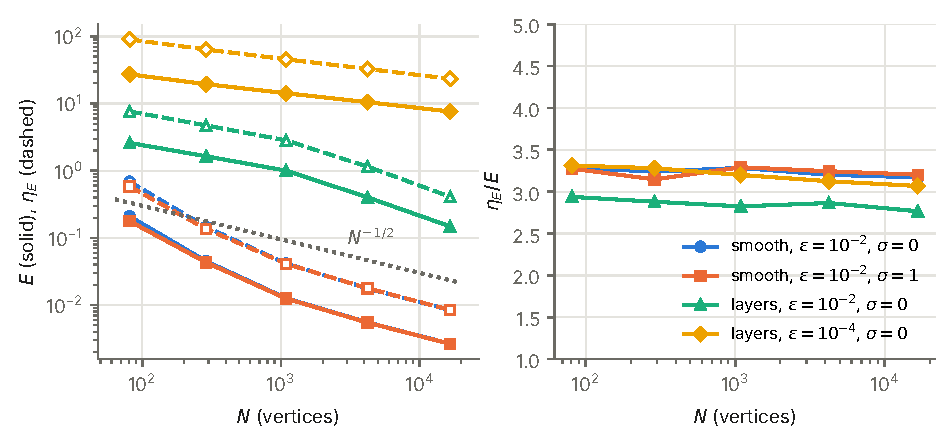
\includegraphics[width=\textwidth]{figures/sv_conv.pdf}
\caption{Uniform refinement in 2D, BJK. Left: $E$ (solid) and $\eta_E$ (dashed, open markers).
Right: effectivity index $I_E=\eta_E/E$.}
\label{fig:conv}
\end{figure}

\subsection{Robustness in \texorpdfstring{$\eps$}{eps}, \texorpdfstring{$\sigma$}{sigma} and the stabilisation}\label{sec:num-robust}

Table~\ref{tab:sweep} and Figure~\ref{fig:sweep} sweep $\eps$ from $10^{-1}$ to $10^{-8}$ on the fixed
mesh $n=32$, for $\sigma\in\{0,1\}$, both stabilisations and both problems.
\begin{itemize}
  \item \textbf{$\sigma=0$.} $I_E$ lies in $2.80$--$3.23$ for the layers problem and in $3.15$--$3.78$
  for the smooth problem, and becomes constant for $\eps\le10^{-5}$. $I_\oplus$ stays below $4.9$,
  and the stabilisation part is estimated sharply, $I_S=1.21$--$1.34$. BJK and SMUAS give the
  same indices $I_E$ and $I_\oplus$ to within $3\,\%$, as Remark~\ref{rem:robust} predicts: the limiter enters only
  through the functional, not the constants.
  \item \textbf{Energy norm.} The energy-norm index $I$ grows like $\eps^{-1}$ for $\sigma=0$, up to
  $2.5\cdot10^6$ at $\eps=10^{-8}$; the guaranteed energy-norm bound of \cite{ABR17} behaves in the
  same way. For $\sigma=1$, $I$ saturates at about $60$--$90$, the reaction giving $L^2$ control, while
  the ABR17 bound keeps growing ($1.3\cdot10^4$ at $\eps=10^{-8}$), because its reaction cut-off is not
  robust.
  \item \textbf{$\sigma=1$, small $\eps$.} Down to $\eps=10^{-6}$, $I_E$ stays in $2.7$--$3.2$ for the
  layers problem and in $3.2$--$4.9$ for the smooth one. For $\eps<10^{-6}$ it rises, to $5.5$ (layers)
  and $6.0$ (smooth) at $\eps=10^{-8}$. This increase comes from $I_S$ ($7.8$ and $10.4$ at
  $\eps=10^{-8}$), while $I_\oplus$ \emph{decreases}. This is consistent with a
  reference effect rather than with a loss of robustness: for $\sigma>0$, the Riesz representative of
  $\Stil$ has layers of width $(\eps/\sigma)^{1/2}=10^{-4}$, far below the mesh size $3\cdot10^{-2}$, so
  the same-mesh $P_2$ reference underestimates $\|\Stil\|_*$. Theorem~\ref{thm:eff} bounds $\eta_S$ by
  the true dual norm, independently of $\eps$. \adapt{The adaptive runs of Section~\ref{sec:num-unad} confirm this:
  once the mesh resolves the layers, $I_S$ falls to $1.5$--$1.6$ and $I_E$ to about $3$.} \asref{The
  asymptotic reference below makes this quantitative.}
\end{itemize}

% generated by examples/convection_diffusion/sv_numerics/make_figures.py; do not edit
\begin{table}[!htbp]
\centering
\footnotesize
\setlength{\tabcolsep}{4pt}
\caption{Robustness in $\eps$ and $\sigma$ on the uniform mesh with $n=32$ ($N=1089$). $I_E=\eta_E/E$, $I_\oplus=\kappa\eta/\tnorm{e}_\oplus$, $I_S=\eta_S/\|\Stil\|_*$, $I=\eta/\tnorm{e}$ and, for comparison, the effectivity $I_{\mathrm{ABR17}}$ of the guaranteed energy-norm bound of \cite{ABR17}.}\label{tab:sweep}
\begin{tabular}{llrrrrrrrr}
\toprule
case & index & $10^{-1}$ & $10^{-2}$ & $10^{-3}$ & $10^{-4}$ & $10^{-5}$ & $10^{-6}$ & $10^{-7}$ & $10^{-8}$\\
\midrule
layers, BJK, $\sigma=0$ & $I_E$ & 2.96 & 2.82 & 3.06 & 3.20 & 3.23 & 3.23 & 3.23 & 3.23\\
 & $I_\oplus$ & 2.98 & 3.56 & 4.30 & 4.75 & 4.84 & 4.84 & 4.84 & 4.84\\
 & $I_S$ & 1.26 & 1.24 & 1.24 & 1.22 & 1.22 & 1.22 & 1.22 & 1.22\\
 & $I$ & 1.06 & 2.21 & 7.95 & 82.17 & $2.5\cdot10^{3}$ & $2.5\cdot10^{4}$ & $2.5\cdot10^{5}$ & $2.5\cdot10^{6}$\\
 & $I_{\mathrm{ABR17}}$ & 1.47 & 1.93 & 6.26 & 64.53 & $1.9\cdot10^{3}$ & $1.9\cdot10^{4}$ & $1.9\cdot10^{5}$ & $1.9\cdot10^{6}$\\
\addlinespace
layers, BJK, $\sigma=1$ & $I_E$ & 3.03 & 3.13 & 3.16 & 2.97 & 2.81 & 3.04 & 3.83 & 5.47\\
 & $I_\oplus$ & 3.05 & 3.95 & 4.25 & 4.02 & 3.83 & 3.50 & 3.28 & 3.24\\
 & $I_S$ & 1.29 & 1.29 & 1.41 & 1.54 & 1.66 & 2.55 & 4.41 & 7.79\\
 & $I$ & 1.09 & 2.33 & 6.39 & 30.27 & 74.58 & 71.78 & 67.57 & 66.77\\
 & $I_{\mathrm{ABR17}}$ & 1.47 & 1.94 & 6.25 & 57.80 & 391.31 & $1.3\cdot10^{3}$ & $4.0\cdot10^{3}$ & $1.3\cdot10^{4}$\\
\addlinespace
layers, SMUAS, $\sigma=0$ & $I_E$ & 2.95 & 2.80 & 3.01 & 3.15 & 3.17 & 3.18 & 3.18 & 3.18\\
 & $I_\oplus$ & 2.97 & 3.57 & 4.29 & 4.73 & 4.82 & 4.82 & 4.82 & 4.82\\
 & $I_S$ & 1.34 & 1.24 & 1.25 & 1.23 & 1.23 & 1.23 & 1.23 & 1.23\\
 & $I$ & 1.06 & 2.26 & 8.09 & 83.92 & $2.7\cdot10^{3}$ & $2.7\cdot10^{4}$ & $2.7\cdot10^{5}$ & $2.7\cdot10^{6}$\\
 & $I_{\mathrm{ABR17}}$ & 1.47 & 1.97 & 6.38 & 65.99 & $2.2\cdot10^{3}$ & $2.2\cdot10^{4}$ & $2.2\cdot10^{5}$ & $2.2\cdot10^{6}$\\
\addlinespace
layers, SMUAS, $\sigma=1$ & $I_E$ & 3.03 & 3.10 & 3.10 & 2.91 & 2.73 & 2.97 & 3.78 & 5.42\\
 & $I_\oplus$ & 3.04 & 3.95 & 4.20 & 4.00 & 3.81 & 3.49 & 3.27 & 3.24\\
 & $I_S$ & 1.37 & 1.28 & 1.41 & 1.50 & 1.61 & 2.46 & 4.26 & 7.53\\
 & $I$ & 1.08 & 2.36 & 6.14 & 28.08 & 66.99 & 64.21 & 60.54 & 59.85\\
 & $I_{\mathrm{ABR17}}$ & 1.47 & 1.99 & 6.38 & 58.84 & 389.93 & $1.3\cdot10^{3}$ & $4.0\cdot10^{3}$ & $1.3\cdot10^{4}$\\
\addlinespace
smooth, BJK, $\sigma=0$ & $I_E$ & 3.15 & 3.28 & 3.76 & 3.78 & 3.58 & 3.58 & 3.58 & 3.58\\
 & $I_\oplus$ & 3.17 & 3.46 & 4.85 & 4.49 & 3.87 & 3.86 & 3.85 & 3.85\\
 & $I_S$ & 1.29 & 1.30 & 1.24 & 1.21 & 1.22 & 1.22 & 1.22 & 1.22\\
 & $I$ & 1.12 & 1.31 & 6.28 & 77.92 & 778.23 & $6.9\cdot10^{3}$ & $6.8\cdot10^{4}$ & $6.8\cdot10^{5}$\\
 & $I_{\mathrm{ABR17}}$ & 1.70 & 1.76 & 5.18 & 74.26 & 842.71 & $7.5\cdot10^{3}$ & $7.4\cdot10^{4}$ & $7.4\cdot10^{5}$\\
\addlinespace
smooth, BJK, $\sigma=1$ & $I_E$ & 3.22 & 3.29 & 3.86 & 4.66 & 4.93 & 4.81 & 5.04 & 6.00\\
 & $I_\oplus$ & 3.24 & 3.46 & 4.82 & 5.50 & 5.68 & 5.22 & 4.79 & 4.69\\
 & $I_S$ & 1.32 & 1.37 & 1.45 & 1.66 & 2.24 & 3.41 & 5.88 & 10.39\\
 & $I$ & 1.14 & 1.29 & 5.60 & 42.08 & 90.00 & 92.63 & 85.82 & 84.22\\
 & $I_{\mathrm{ABR17}}$ & 1.70 & 1.76 & 5.05 & 49.08 & 229.66 & 763.28 & $2.4\cdot10^{3}$ & $7.7\cdot10^{3}$\\
\bottomrule
\end{tabular}
\end{table}


{\color{teal}
\paragraph{An asymptotically exact reference for $\|\Stil\|_*$.} For $\theta\ll1$ the dual norm of the
stabilisation functional can be evaluated without resolving its Riesz representative. With
$q=A\nabla u_h$ cellwise constant, $\Stil(v)=(q,\nabla v)=-\sum_F(\jump{q\cdot n},v)_F$ for $v\in H^1_D$, since
$\dv q=0$ in each cell. Away from the vertices, the Riesz representative is a sum of one-dimensional layers
$-\eps z''+\sigma z=\jump{q\cdot n}\,\delta_F$ across the faces, each of energy
$\jump{q\cdot n}^2/(2(\eps\sigma)^{1/2})$ per unit length. Hence
\begin{equation}\label{eq:Sasym}
  \|\Stil\|_*^2=\sum_{F\text{ interior}}\frac{\|\jump{q\cdot n}\|_F^2}{2(\eps\sigma)^{1/2}}\,\bigl(1+O(\theta)\bigr),
  \qquad \theta\to0,
\end{equation}
and the same sum over the faces interior to $\tilde\omega_K$ gives $\|\Stil\|_{*,\tilde\omega_K}^2$.
Table~\ref{tab:refref} and Figure~\ref{fig:refref} compare this value with $P_2$ references on the same mesh and on
$k$-times refined meshes ($k=2,4,8$), for the layers problem on the $16\times16$ mesh with $\sigma\in\{1,10^4\}$, using
the A+S estimator alone (without the direct variant of Remark~\ref{rem:direct}).
\begin{itemize}
  \item \textbf{The references.} At $\theta=0.11$ the asymptotic value agrees with the refined reference to $1\,\%$
  ($2.92$ against $2.95$). For smaller $\theta$ the $P_2$ references are far from converged: at $\theta=10^{-5}$ the
  same-mesh value underestimates $\|\Stil\|_*$ by a factor $85$, and even the $8$ times refined one by a factor $30$.
  \item \textbf{Theorem~\ref{thm:eff} for $\ell=-\Stil$.} Measured against \eqref{eq:Sasym}, the index
  $I_S=\eta_{-\Stil}/\|\Stil\|_*$ lies in $1.64$--$2.22$ for all $\theta\le10^{-2}$; the local ratio
  $\max_K\eta_{S,K}^2/\|\Stil\|_{*,\tilde\omega_K}^2$ lies in $0.58$--$1.56$. For this functional the theorem has no
  oscillation term, so this is a direct confirmation of robust global and local efficiency in the reaction regime.
  \item \textbf{The error measure.} With $\|\Stil\|_*$ from \eqref{eq:Sasym} and the other two parts of $E$ from the
  $8$ times refined mesh, $\eta_E/E$ stays in $8.3$--$10.2$ over three decades of $\theta$, whereas the same-mesh
  reference gives values up to $284$. The rises of $I_E$ in Table~\ref{tab:sweep} and in Section~\ref{sec:num-unad} at
  small $\theta$ are therefore an artifact of the reference, not a loss of robustness.
\end{itemize}
}

% generated by examples/convection_diffusion/sv_numerics/make_exp36_figures.py; do not edit
\begin{table}[!htbp]
\centering
\small
\setlength{\tabcolsep}{3.5pt}
\caption{\asref{Reaction regime, layers problem, $n=16$, BJK, the A+S estimator alone. $\|\tilde S\|_*$ from $P_2$ on the same mesh ($k=1$), on the $8$ times refined mesh ($k=8$), and the asymptotic value \eqref{eq:Sasym}; $I_S=\eta_{-\tilde S}/\|\tilde S\|_*$; $\eta_E/E$ with the same-mesh reference and with $E^*$, in which $\|\tilde S\|_*$ is the larger of the $k=8$ and the asymptotic value.}}\label{tab:refref}
\begin{tabular}{rrrrrrrrrr}
\toprule
$\sigma$ & $\eps$ & $\theta$ & \multicolumn{3}{c}{$\|\tilde S\|_*$} & \multicolumn{2}{c}{$I_S$} & \multicolumn{2}{c}{$\eta_E/E$}\\
 & & & $k=1$ & $k=8$ & asympt. & $k=8$ & asympt. & $k=1$ & $E^*$\\
\midrule
1 & $10^{-2}$ & $1.1$ & 0.461 & 0.461 & 0.564 & 1.34 & 1.10 & 3.4 & 3.1 \\
1 & $10^{-4}$ & $1.1\cdot10^{-1}$ & 2.67 & 2.95 & 2.92 & 1.72 & 1.73 & 5.6 & 5.1 \\
1 & $10^{-6}$ & $1.1\cdot10^{-2}$ & 3.34 & 8.14 & 9.28 & 2.49 & 2.19 & 15.6 & 8.4 \\
1 & $10^{-8}$ & $1.1\cdot10^{-3}$ & 3.35 & 9.77 & 29.4 & 5.33 & 1.77 & 43.5 & 9.3 \\
10000 & $10^{-2}$ & $1.1\cdot10^{-2}$ & 5.02 & 11.9 & 13.5 & 2.52 & 2.22 & 14.0 & 8.3 \\
10000 & $10^{-4}$ & $1.1\cdot10^{-3}$ & 5.29 & 15.2 & 45 & 5.36 & 1.81 & 30.4 & 9.0 \\
10000 & $10^{-6}$ & $1.1\cdot10^{-4}$ & 5.29 & 15.2 & 142 & 15.68 & 1.68 & 91.1 & 9.9 \\
10000 & $10^{-8}$ & $1.1\cdot10^{-5}$ & 5.29 & 15.2 & 450 & 48.39 & 1.64 & 283.6 & 10.2 \\
\bottomrule
\end{tabular}
\end{table}


\begin{figure}[!htbp]
\centering
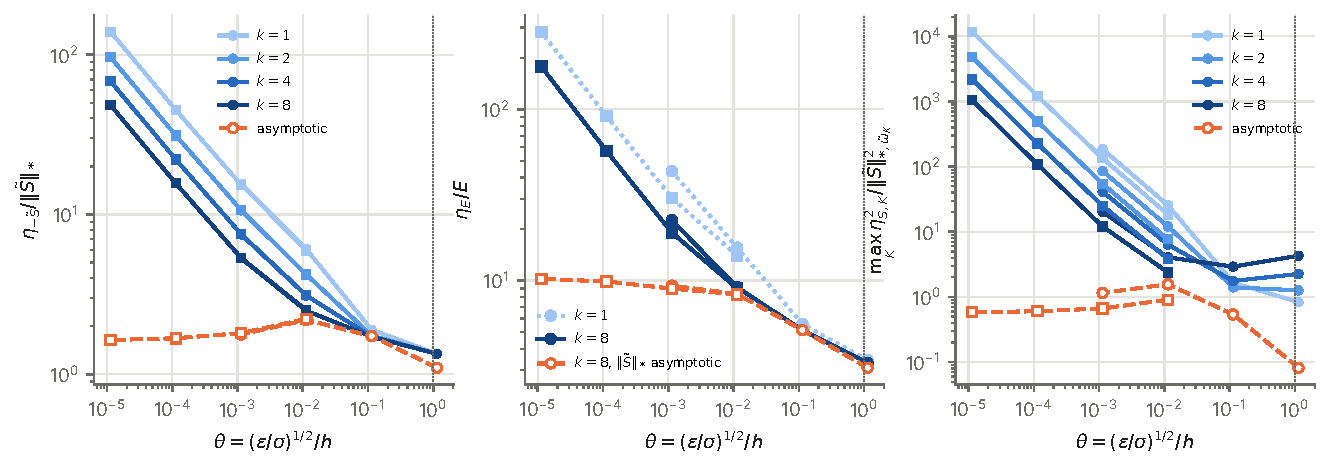
\includegraphics[width=\textwidth]{figures/sv_refref.pdf}
\caption{\asref{Reaction regime, layers problem, $n=16$, A+S estimator; circles $\sigma=1$, squares $\sigma=10^4$.
Left: $\eta_{-\Stil}/\|\Stil\|_*$ with $P_2$ references on $k$-times refined meshes and with the asymptotic value
\eqref{eq:Sasym}. Middle: $\eta_E/E$ with the same-mesh and the $8$ times refined references, and with
$\|\Stil\|_*$ from \eqref{eq:Sasym}. Right: the local ratio for $\ell=-\Stil$; the refined references are lower bounds
of the local dual norms, so these ratios are upper estimates; the asymptotic value is valid only for $\theta\ll1$.}}
\label{fig:refref}
\end{figure}

\begin{figure}[!htbp]
\centering
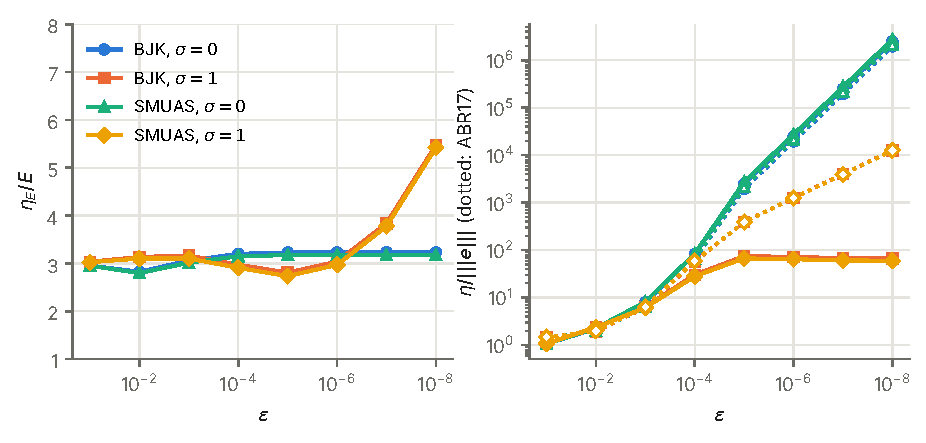
\includegraphics[width=\textwidth]{figures/sv_sweep.pdf}
\caption{Layers problem, $n=32$, as functions of $\eps$. Left: $I_E=\eta_E/E$. Right: the energy-norm
indices $\eta/\tnorm{e}$ (solid) and, dotted with open markers, that of the guaranteed bound of
\cite{ABR17}.}
\label{fig:sweep}
\end{figure}

\subsection{Variable reaction}\label{sec:num-cb}

With $c=1+(c_{\max}-1)xy$ and $\sigma=1$, the constant of (H3) is $\|c\|_\infty/\sigma=c_{\max}$, attained at
the vertex $(1,1)$. \refe{The computed $c_b$ is the sampled enclosure of Remark~\ref{rem:CF}, which is diagnostic: $c$ is not
affine on the cells, so the sampled maximum is enlarged by $\frac{h_K}2\max|\nabla c|$; here this gives} $c_b=1.12\,c_{\max}$, $1.06\,c_{\max}$
and $1.03\,c_{\max}$ for $n=8,16,32$, and $\kappa=2+c_b$ (Table~\ref{tab:cb}). The bound $E\le\eta_E$ holds in
all runs. The index of $\eta_{E,c}$ grows at most linearly, $\eta_{E,c}/E_c\le3\,c_b$ in all runs, as
Corollary~\ref{cor:twoc} predicts; it is often much smaller, down to $0.05\,c_b$, because the factor $M=c_b$ in front of $\tnorm{e}$ in $E_c$ also enlarges the
error measure. The index of $\eta_E$ grows faster, up to $5.2\,c_b$ at $c_b\approx10^3$, but stays far
below the worst case $(1+c_b)^2$ of Corollary~\ref{cor:two}. A variable reaction with a small lower
bound $\sigma$ is therefore the one situation in which the estimator loses its robustness, in
accordance with the theory; Section~\ref{sec:concl} discusses how to remove it.

% generated by examples/convection_diffusion/sv_numerics/make_figures.py; do not edit
\begin{table}[!htbp]
\centering
\small
\setlength{\tabcolsep}{4pt}
\caption{Variable reaction $c=1+(c_{\max}-1)xy$, $\sigma=1$, $\eps\in\{10^{-3},10^{-6}\}$, $n\in\{8,16,32\}$: ranges over the six runs; $c_b$ and $\kappa$ are the means of the sampled enclosures (Remark~\ref{rem:CF}; diagnostic), which exceed $c_{\max}$ by $3$--$12\,\%$.}\label{tab:cb}
\begin{tabular}{rrrllll}
\toprule
$c_{\max}$ & $c_b$ & $\kappa$ & $\eta_E/E$ & $\eta_{E,c}/E_c$ & $\eta_{E,c}/(c_bE_c)$ & $E\le\eta_E$\\
\midrule
1 & 1.00 & 3.00 & 3.85--5.34 & 3.85--5.34 & 3.85--5.34 & yes\\
10 & 10.66 & 12.66 & 14.63--19.94 & 8.69--30.35 & 0.85--2.95 & yes\\
100 & 107.22 & 109.22 & 128--271 & 12.27--216 & 0.12--2.09 & yes\\
1000 & $1.1\cdot10^{3}$ & $1.1\cdot10^{3}$ & 1618--5312 & 56.23--1125 & 0.05--1.09 & yes\\
\bottomrule
\end{tabular}
\end{table}


\subsection{Local efficiency}\label{sec:num-loc}

Table~\ref{tab:loc} reports the localised measure for the layers problem on the $16\times16$ mesh. The
local ratio $\max_K\eta_K^2/E_{\mathrm{loc}}(\tilde\omega_K)^2$ is at most $0.51$ in all cases, and
independent of $\eps$ for $\eps\le10^{-4}$: the estimator is locally efficient, as stated in
Theorem~\ref{thm:loc}. The ratio $E_{\mathrm{loc}}/E$ lies between $0.48$ and $1.01$, so on these
problems the localised measure captures most of the global one, and the guaranteed bound
$E_{\mathrm{loc}}\le\sqrt{d+1}\,\eta_E$ of Theorem~\ref{thm:loc} overestimates $E_{\mathrm{loc}}$ by a
factor $5$--$12$. The largest value, $\eta_E/E_{\mathrm{loc}}=7.0$ for $\sigma=1$ and $\eps=10^{-8}$, is the
same reference effect as in Section~\ref{sec:num-robust}.

% generated by examples/convection_diffusion/sv_numerics/make_figures.py; do not edit
\begin{table}[!htbp]
\centering
\small
\setlength{\tabcolsep}{4pt}
\caption{Localised measure (Theorem~\ref{thm:loc}), outflow layers, BJK, $n=16$. The last but one column is $\max_K\eta_K^2/E_{\mathrm{loc}}(\tilde\omega_K)^2$ with $\eta_K=\eta_{A,K}+\eta_{S,K}$.}\label{tab:loc}
\begin{tabular}{rrrrrrr}
\toprule
$\sigma$ & $\eps$ & $E_{\mathrm{loc}}/E$ & $\eta_E/E_{\mathrm{loc}}$ & $\sqrt{d+1}\,\eta_E/E_{\mathrm{loc}}$ & local max & $I_E$\\
\midrule
0 & $10^{-2}$ & 0.48 & 5.94 & 10.29 & 0.26 & 2.88\\
0 & $10^{-4}$ & 0.60 & 5.50 & 9.53 & 0.37 & 3.28\\
0 & $10^{-6}$ & 0.60 & 5.50 & 9.52 & 0.37 & 3.29\\
0 & $10^{-8}$ & 0.60 & 5.50 & 9.52 & 0.37 & 3.29\\
1 & $10^{-2}$ & 0.52 & 6.38 & 11.05 & 0.51 & 3.33\\
1 & $10^{-4}$ & 0.95 & 3.07 & 5.32 & 0.13 & 2.93\\
1 & $10^{-6}$ & 1.01 & 3.47 & 6.01 & 0.07 & 3.51\\
1 & $10^{-8}$ & 1.01 & 7.04 & 12.20 & 0.07 & 7.13\\
\bottomrule
\end{tabular}
\end{table}


\subsection{Adaptive refinement}\label{sec:num-adapt}

Starting from the $8\times8$ mesh, we mark by the indicators $\eta_K=\eta_{A,K}+\eta_{S,K}$ with the
dual strategy of \cite{AJ27} (all cells with $\eta_K\ge\theta\max\eta$, $\theta=0.5$, reduced until at least
$5\,\%$ of the cells are marked) and refine by red--green refinement, until $N>3\cdot10^4$.
Table~\ref{tab:adapt} and Figures~\ref{fig:adapt} and~\ref{fig:adaptmesh} show the results for the layers
problem.
\begin{itemize}
  \item \textbf{Effectivity.} $I_E$ stays between $2.86$ and $3.55$ in every loop of all three runs, from
  $N=81$ to $N=45\,094$, while the local mesh size spans three orders of magnitude.
  \item \textbf{Where the mesh is refined.} The refinement concentrates in the outflow layers at $x=1$ and
  $y=1$ (Figure~\ref{fig:adaptmesh}); the smallest cells have $h_{\min}=3.5\cdot10^{-4}$ for $\eps=10^{-3}$,
  below $\eps$, so the layers are resolved, and $h_{\min}=1.7\cdot10^{-4}$ for $\eps=10^{-5}$, where they are not.
  \item \textbf{Convergence.} For $\eps=10^{-3}$, $E$ decreases at the rate $1.8$--$1.9$ with respect to
  $N^{-1/2}$ over the second half of the loops: this is the pre-asymptotic phase in which the layers become
  resolved, faster than the optimal rate $1$. For $\eps=10^{-5}$ the rate is $0.98$. On the finest uniform mesh
  ($N=16\,641$) the error $E$ is $18$, $4.4$ and $17$ times larger than the adaptive error at the same $N$.
  Under uniform refinement $E$ decreases at the rate $0.46$--$0.60$ for $\sigma=0$ and $0.04$--$0.51$ for
  $\sigma=1$, because the layers are never resolved; the index $I_E$ is $2.86$--$3.37$ there as well.
  \item \textbf{Energy norm.} Along the adaptive runs the energy-norm index $I$ falls from $29$ to $1.1$
  ($\eps=10^{-3}$) and from $8.4\cdot10^3$ to $6.2$ ($\eps=10^{-5}$): once the mesh resolves the layers, the
  energy error and the dual norm of the residual become comparable, while $I_E$ is insensitive to this.
\end{itemize}

% generated by examples/convection_diffusion/sv_numerics/make_figures.py; do not edit
\begin{table}[!htbp]
\centering
\small
\setlength{\tabcolsep}{4pt}
\caption{Adaptive refinement for the outflow-layers problem, BJK, dual marking by the SV indicators $\eta_K$, red--green refinement. The rate is that of $E$ with respect to $N^{-1/2}$ over the second half of the loops; the last column is the ratio of $E$ on the finest uniform mesh ($N=16641$) to the adaptive $E$ at the same $N$.}\label{tab:adapt}
\begin{tabular}{rrrrllrlr}
\toprule
$\eps$ & $\sigma$ & loops & $N$ (last) & $h_{\min}$ & $E$ (last) & rate & $\eta_E/E$ & gain\\
\midrule
$10^{-3}$ & 0 & 15 & 33010 & $3.45\cdot10^{-4}$ & $7.395\cdot10^{-2}$ & 1.88 & 2.86--3.25 & 18.3\\
$10^{-5}$ & 0 & 12 & 31866 & $1.73\cdot10^{-4}$ & $3.941$ & 0.98 & 2.94--3.35 & 4.4\\
$10^{-3}$ & 1 & 17 & 45094 & $1.73\cdot10^{-4}$ & $5.891\cdot10^{-2}$ & 1.83 & 2.96--3.55 & 17.2\\
\bottomrule
\end{tabular}
\end{table}


\begin{figure}[!htbp]
\centering
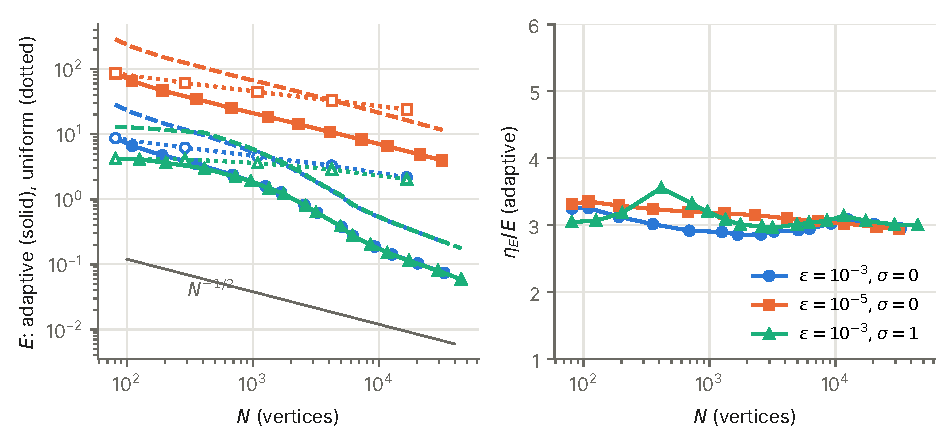
\includegraphics[width=\textwidth]{figures/sv_adapt.pdf}
\caption{Adaptive refinement, layers problem, BJK. Left: $E$ for adaptive (solid) and uniform (dotted, open
markers) refinement, and $\eta_E$ for the adaptive runs (dashed). Right: $I_E$ along the adaptive runs.}
\label{fig:adapt}
\end{figure}

\begin{figure}[!htbp]
\centering
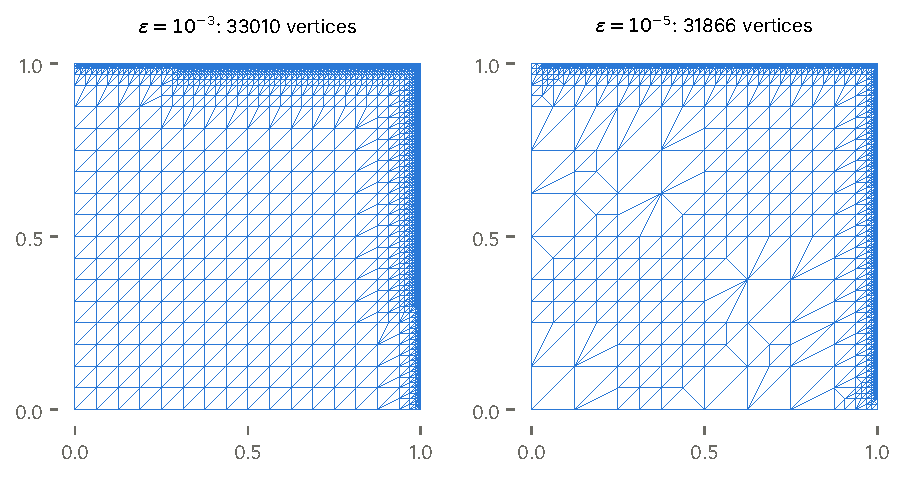
\includegraphics[width=\textwidth]{figures/sv_adapt_mesh.pdf}
\caption{Final adaptive meshes, layers problem, $\sigma=0$.}
\label{fig:adaptmesh}
\end{figure}

\subsection{\adapt{Uniform versus adaptive refinement}}\label{sec:num-unad}
{\color{magenta}

We repeat the uniform-mesh studies of Tables~\ref{tab:conv} and~\ref{tab:sweep} with adaptive refinement:
the same problems, the same marking as in Section~\ref{sec:num-adapt}, from the $8\times8$ mesh up to
$N\approx2\cdot10^4$ (Table~\ref{tab:conv}) and $N\approx10^4$ (Table~\ref{tab:sweep}). For the robustness
sweep we compare at equal cost: the adaptive loop whose $N$ is closest to $N=1089$, the size of the $32\times32$
mesh of Table~\ref{tab:sweep}.

\paragraph{Refinement studies (Figure~\ref{fig:aconv}).}
\begin{itemize}
  \item \textbf{Effectivity.} Along the adaptive runs $I_E$ lies in $2.83$--$4.18$ and tends to the same values
  as on uniform meshes, about $3.0$--$3.2$. The bound held in every loop.
  \item \textbf{Accuracy.} For the smooth solution, adaptive refinement gains nothing: at $N=16\,641$ the two
  errors agree to within $1\,\%$, and $E$ converges at the rate $1$ in both cases. For the layers problem the
  uniform error is $5.4$ ($\eps=10^{-2}$) and $5.9$ ($\eps=10^{-4}$) times the adaptive one at the same $N$.
  For $\eps=10^{-4}$, $E$ converges at the rate $0.47$ under uniform refinement and at $1.4$--$1.9$ in the last
  adaptive loops, in which the layers become resolved.
\end{itemize}

\begin{figure}[!htbp]
\centering
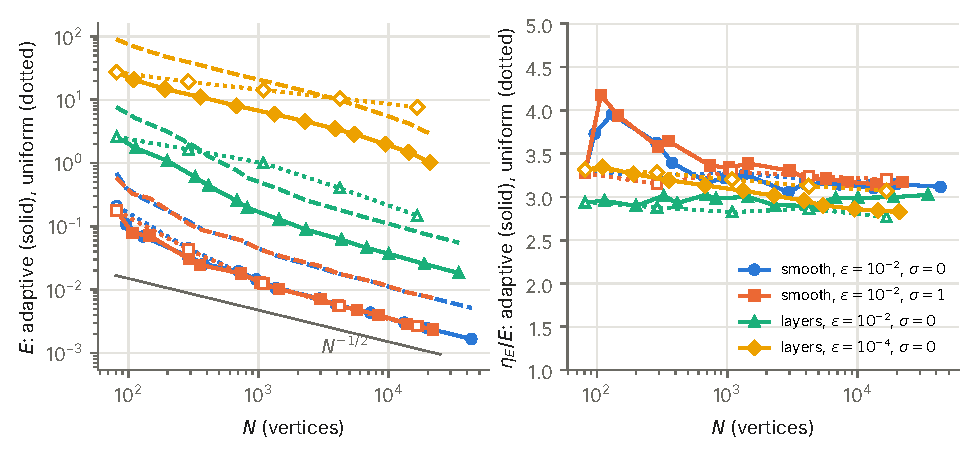
\includegraphics[width=\textwidth]{figures/sv_aconv.pdf}
\caption{\adapt{The cases of Table~\ref{tab:conv} under adaptive refinement. Left: $E$ for adaptive (solid) and uniform
(dotted, open markers) refinement, and $\eta_E$ for the adaptive runs (dashed). Right: $I_E$, adaptive (solid) and
uniform (dotted).}}
\label{fig:aconv}
\end{figure}

\paragraph{Robustness sweep (Figures~\ref{fig:abudget} and~\ref{fig:aloops}).}
\begin{itemize}
  \item \textbf{$\sigma=0$.} At equal cost, $I_E=2.89$--$3.22$ on the adaptive meshes against $2.80$--$3.23$ on the
  uniform mesh, for all $\eps$ and both stabilisations, and it stays in $2.82$--$3.35$ over all loops: the
  estimator is as robust on the meshes it generates as on the fixed mesh.
  \item \textbf{$\sigma=1$, small $\eps$.} The rise of $I_E$ to $5.4$--$5.5$ on the uniform mesh at
  $\eps\le10^{-7}$ (Section~\ref{sec:num-robust}) does not occur at equal cost on the adaptive meshes, where
  $I_E=2.75$--$3.16$. Figure~\ref{fig:aloops} shows why. The large values, up to $9.6$, appear only on the
  coarse initial mesh, and they come from the stabilisation part: $I_S=17.8$ at $N=81$ for $\eps=10^{-8}$. As the
  mesh resolves the layers, $I_S$ falls to $1.5$--$1.6$ and $I_E$ returns to about $3$. This confirms that the
  rise on the uniform mesh is a property of the under-resolved $P_2$ reference for $\|\Stil\|_*$, not of the
  estimator.
  \item \textbf{Smooth problem.} For $\eps\le10^{-3}$ the adaptive indices are higher than the uniform ones at
  equal cost: $I_E=4.0$--$5.3$ against $3.6$--$3.8$ for $\sigma=0$, and $4.5$--$6.0$ against $3.9$--$6.0$ for
  $\sigma=1$. Along the runs they reach $7.8$ after the first loop, and $10.9$ on the initial mesh. For $\sigma=1$
  and $\eps\le10^{-6}$ the fixed-point iteration reaches the iteration limit $2\cdot10^4$ on most meshes beyond
  $N\approx1100$, and the bound holds at these iterates.
  \item \textbf{Energy norm.} At $\sigma=0$ the energy-norm index still grows like $\eps^{-1}$ on the adaptive meshes,
  to $4\cdot10^5$ at $\eps=10^{-8}$ (uniform: $2.5\cdot10^6$); only the augmented measure is robust.
  \item \textbf{An open point.} For the layers problem with $\sigma=1$ and $\eps=10^{-6}$, $I_E$ rises again in the
  last loops, from $2.8$ to $4.3$, together with $I_\oplus$ (from $3.2$ to $6.6$). We have not identified the cause;
  it may be the convective part of the reference becoming resolved, and would need runs beyond $N=10^4$.
\end{itemize}

\begin{figure}[!htbp]
\centering
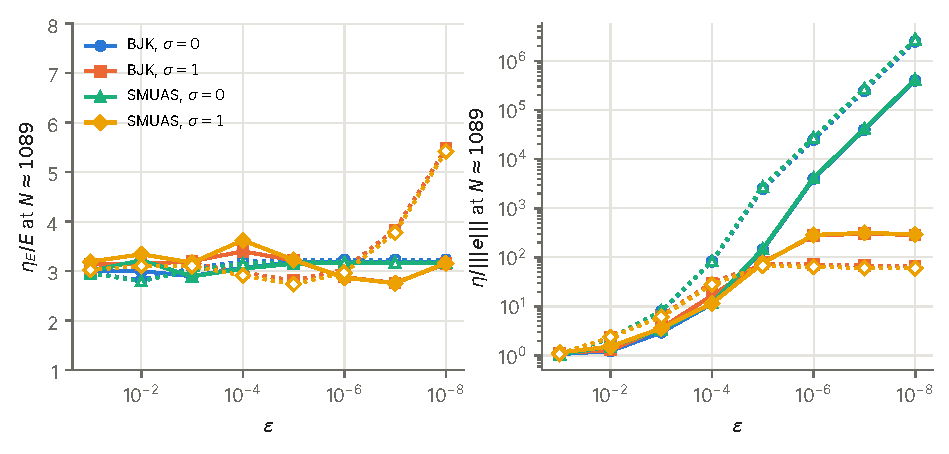
\includegraphics[width=\textwidth]{figures/sv_asweep_budget.pdf}
\caption{\adapt{The robustness sweep of Table~\ref{tab:sweep} at equal cost, layers problem: adaptive meshes with
$N\approx1089$ (solid) against the uniform $32\times32$ mesh (dotted, open markers). Left: $I_E$. Right: the
energy-norm index $\eta/\tnorm{e}$.}}
\label{fig:abudget}
\end{figure}

\begin{figure}[!htbp]
\centering
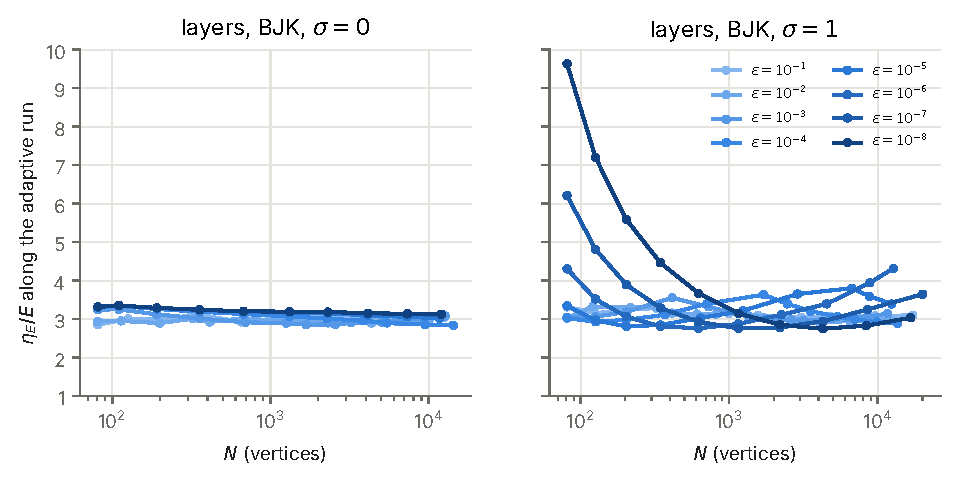
\includegraphics[width=\textwidth]{figures/sv_asweep_loops.pdf}
\caption{\adapt{$I_E$ along the adaptive runs of the robustness sweep, layers problem, BJK; one line per $\eps$, darker for
smaller $\eps$.}}
\label{fig:aloops}
\end{figure}

\paragraph{Which refinement to use.} For computing solutions, adaptive refinement is clearly preferable when the
solution has layers, by factors $4$--$18$ in $E$ at equal $N$, and it is what the estimator is designed for. For
testing the theory, the uniform meshes remain the primary evidence: a fixed coarse mesh keeps the layers
unresolved, which is the regime in which robustness can fail, isolates the dependence on $\eps$ and $\sigma$, and
is the only setting in which rates in $h$ are meaningful. The adaptive runs confirm that the effectivity stays at
about $3$ on the meshes the estimator generates itself.
}% end of the magenta block

\subsection{Inexact iterates and adaptive stopping}\label{sec:num-stop}

\paragraph{Iterates.} Table~\ref{tab:iter} and Figure~\ref{fig:iter} evaluate the estimator at the
fixed-point iterates $u^i$ on the $16\times16$ mesh. The index $I_E$ stays between $2.9$ and $5.3$ at
every iterate, including the first one, where the algebraic part $\eta_{\mathrm{alg}}$ is up to $71\,\%$
of $\eta_{\mathrm{disc}}$: this is part~2 of Proposition~\ref{prop:stop}, efficiency at every iterate
without any condition on the algebraic error. The ratio $\eta_{\mathrm{alg}}/\eta_{\mathrm{disc}}$
decreases monotonically for all problems except the smooth one with $\eps=10^{-6}$ and $\sigma=0$, for
which the fixed-point iteration does not converge in $2\cdot10^4$ iterations; there the ratio stalls
between $10^{-3}$ and $4\cdot10^{-3}$. In that case the error is smallest at $i\approx10$, $E(u^{10})=4.8$, and grows to
$8.4$ at $i=2\cdot10^4$: further iterations make the iterate worse in $E$, and the estimator, which is
efficient at every iterate, reflects this.

% generated by examples/convection_diffusion/sv_numerics/make_figures.py; do not edit
\begin{table}[!htbp]
\centering
\small
\setlength{\tabcolsep}{4pt}
\caption{Fixed-point iterates $u^i$, $i\in\{1,2,5,\dots,1000\}$ below the converged count, and the converged solution; BJK, $n=16$. The split is $\eta_{\mathrm{disc}}=\eta_E-\eta_{\mathrm{alg}}$.}\label{tab:iter}
\begin{tabular}{lrrrlrrl}
\toprule
problem & $\eps$ & $\sigma$ & it.\ to tol. & $\eta_E/E$ over $i$ & $\max_i\eta_{\mathrm{alg}}/\eta_{\mathrm{disc}}$ & $E(u^1)/E(u^{\mathrm{last}})$ & $E\le\eta_E$\\
\midrule
smooth & $10^{-2}$ & 0 & 39 & 3.24--3.63 & 0.71 & 1.81 & yes\\
smooth & $10^{-2}$ & 1 & 37 & 3.15--3.45 & 0.51 & 1.58 & yes\\
smooth & $10^{-6}$ & 0 & 20000 & 3.76--4.61 & 0.58 & 1.06 & yes\\
smooth & $10^{-6}$ & 1 & 664 & 4.42--5.28 & 0.19 & 1.20 & yes\\
layers & $10^{-2}$ & 0 & 47 & 2.88--2.97 & 0.02 & 1.01 & yes\\
layers & $10^{-2}$ & 1 & 45 & 3.32--3.33 & 0.01 & 1.01 & yes\\
layers & $10^{-6}$ & 0 & 635 & 3.29--3.47 & 0.04 & 1.01 & yes\\
layers & $10^{-6}$ & 1 & 502 & 3.51--3.56 & 0.02 & 1.03 & yes\\
\bottomrule
\end{tabular}
\end{table}


\begin{figure}[!htbp]
\centering
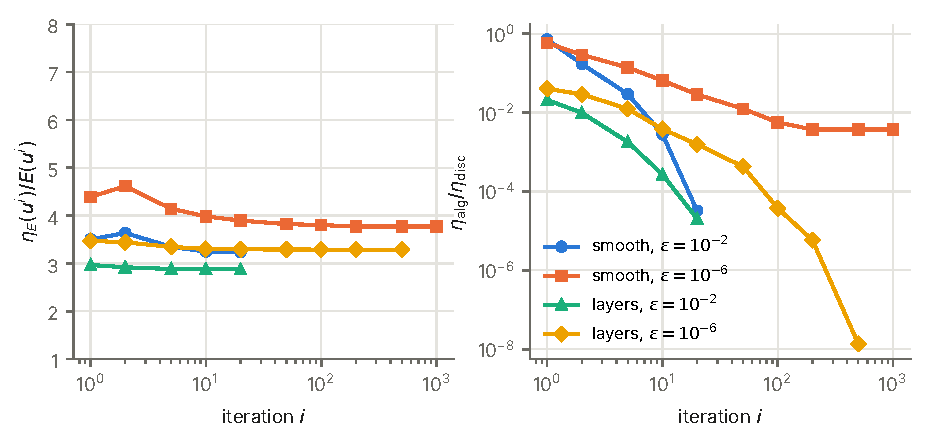
\includegraphics[width=\textwidth]{figures/sv_iter.pdf}
\caption{Fixed-point iterates, BJK, $\sigma=0$, $n=16$. Left: $I_E$ at the iterate $u^i$. Right: the
ratio $\eta_{\mathrm{alg}}/\eta_{\mathrm{disc}}$ (points with a ratio below $10^{-8}$ are omitted).}
\label{fig:iter}
\end{figure}

\paragraph{Adaptive stopping.} Table~\ref{tab:stop} runs five adaptive loops \refe{as in} Section~\ref{sec:num-adapt}
in which the fixed-point iteration is stopped either at the fixed tolerance $\|r\|\le10^{-10}\sqrt N$ or by
the criterion \eqref{eq:stop}, $\eta_{\mathrm{alg}}\le\gamma\eta_{\mathrm{disc}}$, with
$\eta_{\mathrm{disc}}=\eta_E-\eta_{\mathrm{alg}}$; each loop starts from the zero initial guess.
\begin{itemize}
  \item \textbf{Savings.} With $\gamma=0.1$, the total number of iterations drops from $227$ to $25$ (smooth,
  $\eps=10^{-2}$) and from $2323$ to $25$ (layers, $\eps=10^{-4}$), by factors $9$ and $93$; with $\gamma=0.01$
  the factors are $4.5$ and $46$.
  \item \textbf{Accuracy.} The final error $E$ changes by at most $6\,\%$ ($\gamma=0.1$, layers) and by at most
  $0.3\,\%$ for $\gamma\le0.01$. The index $I_E$ stays in $3.1$--$4.8$ in all runs, and in every stopped loop
  $\eta_{\mathrm{alg}}/\eta_{\mathrm{disc}}\le\gamma$, so $E\le(1+\gamma)\eta_{\mathrm{disc}}$
  (Proposition~\ref{prop:stop}, part~3).
  \item \textbf{Non-converging iteration.} For the smooth problem with $\eps=10^{-6}$ the fixed-point
  iteration does not reach the tolerance within $10^4$ iterations on any mesh, and $50\,000$ iterations give
  $E=3.22$. The criterion with $\gamma=0.1$ stops after $5$--$15$ iterations per loop, $50$ in total, with a
  \emph{smaller} error, $E=1.98$: as in Figure~\ref{fig:iter}, the early iterates are better than the late
  ones. For $\gamma=10^{-3}$ the criterion fires in only one of the five loops, since $\eta_{\mathrm{alg}}/\eta_{\mathrm{disc}}$ stalls
  at about $3\cdot10^{-3}$; this is a property of the iteration, not of the estimator.
\end{itemize}

% generated by examples/convection_diffusion/sv_numerics/make_figures.py; do not edit
\begin{table}[!htbp]
\centering
\footnotesize
\setlength{\tabcolsep}{4pt}
\caption{Adaptive stopping in five adaptive loops (dual marking by the SV indicators, red--green refinement), BJK, $\sigma=0$. ``tol.'' is the fixed tolerance $\|r\|\le10^{-10}\sqrt N$; otherwise the iteration stops at $\eta_{\mathrm{alg}}\le\gamma\eta_{\mathrm{disc}}$ (at most $10^4$ iterations). The last column says whether every loop stopped before the iteration limit.}\label{tab:stop}
\begin{tabular}{lrrrrlllr}
\toprule
problem & $\eps$ & $\gamma$ & it./loop & total & $E$ (last) & $\eta_E/E$ & $\max\eta_{\mathrm{alg}}/\eta_{\mathrm{disc}}$ & stopped\\
\midrule
smooth & $10^{-2}$ & tol. & 30--59 & 227 & $2.550\cdot10^{-2}$ & 3.29--3.95 & $5.78\cdot10^{-8}$ & yes\\
smooth & $10^{-2}$ & 0.1 & 5 & 25 & $2.554\cdot10^{-2}$ & 3.41--3.97 & $5.07\cdot10^{-2}$ & yes\\
smooth & $10^{-2}$ & 0.01 & 10 & 50 & $2.551\cdot10^{-2}$ & 3.33--3.98 & $7.27\cdot10^{-3}$ & yes\\
smooth & $10^{-2}$ & 0.001 & 10--20 & 80 & $2.551\cdot10^{-2}$ & 3.29--3.96 & $9.89\cdot10^{-4}$ & yes\\
smooth & $10^{-6}$ & tol. & 10000 & 50000 & $3.218$ & 3.77--4.58 & $3.03\cdot10^{-3}$ & no\\
smooth & $10^{-6}$ & 0.1 & 5--15 & 50 & $1.984$ & 4.04--4.79 & $9.83\cdot10^{-2}$ & yes\\
smooth & $10^{-6}$ & 0.01 & 120--760 & 2190 & $2.749$ & 3.80--4.45 & $9.10\cdot10^{-3}$ & yes\\
smooth & $10^{-6}$ & 0.001 & 7320--10000 & 47320 & $3.218$ & 3.77--4.58 & $3.03\cdot10^{-3}$ & no\\
layers & $10^{-4}$ & tol. & 385--628 & 2323 & $8.044$ & 3.13--3.34 & $3.57\cdot10^{-9}$ & yes\\
layers & $10^{-4}$ & 0.1 & 5 & 25 & $8.524$ & 3.20--3.42 & $2.49\cdot10^{-2}$ & yes\\
layers & $10^{-4}$ & 0.01 & 10 & 50 & $8.023$ & 3.15--3.38 & $8.43\cdot10^{-3}$ & yes\\
layers & $10^{-4}$ & 0.001 & 25--50 & 175 & $8.04$ & 3.14--3.35 & $9.29\cdot10^{-4}$ & yes\\
\bottomrule
\end{tabular}
\end{table}


\subsection{Variable diffusion}\label{sec:num-vareps}

Table~\ref{tab:vareps} reports the variable-diffusion problems on the meshes $n=8,16,32$. All bounds are
guaranteed. For the smooth coefficient, the oscillation $\eta_\eps$ converges at the rate $2.09$--$2.13$
in $h$, in accordance with Lemma~\ref{lem:V}(iii), and is at most $12\,\%$ of $\eta$ (at contrast $10^4$ on
the coarsest mesh). For the jump aligned with the mesh, $\Pi_1\eps=\eps$ and $\eta_\eps=0$. The
effectivity $I_E$ lies in $2.6$--$4.5$ for contrasts up to $10^4$, for $\eps=10^{-2}$ and $10^{-6}$ alike. For
the jump it does not grow with the contrast; for the smooth coefficient it grows mildly, from
$3.1$ at contrast $1$ to at most $4.3$ at contrast $10^4$ (on the coarsest mesh). This is the quasi-monotone case; the constants of
Theorem~\ref{thm:vareps} depend on the patch contrast, but for an aligned jump that contrast does not
show up in the indices. Checkerboard (non-quasi-monotone) coefficients are not tested; for them no
local estimator can be robust \cite{Li26}.

% generated by examples/convection_diffusion/sv_numerics/make_figures.py; do not edit
\begin{table}[!htbp]
\centering
\footnotesize
\setlength{\tabcolsep}{4pt}
\caption{Variable diffusion, BJK, $\sigma=0$, $n\in\{8,16,32\}$: ranges over the three meshes. The rate is that of $\eta_\eps$ with respect to $N^{-1/2}$ between $n=16$ and $n=32$ (expected: $2$).}\label{tab:vareps}
\begin{tabular}{lrrllllrl}
\toprule
$\eps(x)$ & $\eps$ & contrast & $I$ & $I_\oplus$ & $I_E$ & $\max\eta_\eps/\eta$ & rate & $E\le\eta_E$\\
\midrule
smooth & $10^{-2}$ & 1 & 1.23--4.58 & 3.30--4.06 & 3.07--3.13 & 0.000 & --- & yes\\
smooth & $10^{-2}$ & 100 & 1.07--1.24 & 3.16--3.39 & 3.15--3.26 & 0.035 & 2.09 & yes\\
smooth & $10^{-2}$ & 10000 & 1.10--1.44 & 3.30--4.28 & 3.29--4.27 & 0.117 & 2.09 & yes\\
smooth & $10^{-6}$ & 1 & 7959--36796 & 3.72--5.01 & 3.50--3.70 & 0.000 & --- & yes\\
smooth & $10^{-6}$ & 100 & 818--3354 & 3.73--5.44 & 3.54--4.03 & 0.000 & 2.13 & yes\\
smooth & $10^{-6}$ & 10000 & 64.07--336 & 4.31--5.49 & 3.94--4.46 & 0.001 & 2.10 & yes\\
jump & $10^{-2}$ & 100 & 2.56--7.63 & 3.43--4.18 & 2.61--2.99 & 0.000 & --- & yes\\
jump & $10^{-2}$ & 10000 & 2.61--8.12 & 3.43--4.22 & 2.60--3.01 & 0.000 & --- & yes\\
jump & $10^{-6}$ & 100 & 9025--28125 & 4.75--5.12 & 3.44--3.54 & 0.000 & --- & yes\\
jump & $10^{-6}$ & 10000 & 2156--4989 & 4.78--5.08 & 3.41--3.52 & 0.000 & --- & yes\\
\bottomrule
\end{tabular}
\end{table}


\subsection{Three dimensions}\label{sec:num-3d}

Table~\ref{tab:d3} repeats the uniform-refinement study on the unit cube ($n=4,8,16$, up to $N=4913$
vertices and $24\,576$ tetrahedra).
\begin{itemize}
  \item \textbf{Layers.} $I_E=2.94$--$3.55$ for $\eps=10^{-2}$ and $10^{-6}$, as in two dimensions; $I_\oplus\le4.9$
  and $I_S=1.21$--$1.26$.
  \item \textbf{Smooth solution.} $I_E$ is higher than in two dimensions, $5.1$--$6.4$, but decreases under
  refinement for both values of $\eps$ ($5.97\to5.40$ and $6.39\to5.09$). These meshes are coarse: $E$ still
  converges at the pre-asymptotic rates $2.1$--$2.7$ in $h$, dominated by the stabilisation part
  $\|\Stil\|_*$, which is estimated sharply ($I_S=1.28$--$1.31$); the larger index comes from the convective
  dual norm on coarse tetrahedral meshes. For $\eps=10^{-6}$ on the finest mesh the fixed-point iteration does
  not converge within $2\cdot10^4$ iterations, and the bound still holds at the last iterate.
  \item \textbf{Energy norm.} As in two dimensions, $I$ is useless for $\sigma=0$ and small $\eps$
  ($1.0\cdot10^4$--$1.4\cdot10^5$ at $\eps=10^{-6}$, against $2.6$--$9.3$ at $\eps=10^{-2}$), while $I_E$ is not
  affected.
  \item \textbf{Cost.} The estimator takes about $8$\,s at $N=729$ and $220$--$240$\,s at $N=4913$ in our
  Python implementation; the cost is dominated by the vertex-patch problems in $\RTN$, whose size grows
  quickly with the number of tetrahedra per patch in three dimensions. The patch problems are independent and
  can be solved in parallel; the global $\RT_0$ defect problem takes a small fraction of the time.
\end{itemize}

% generated by examples/convection_diffusion/sv_numerics/make_figures.py; do not edit
\begin{table}[!htbp]
\centering
\small
\setlength{\tabcolsep}{4pt}
\caption{Three dimensions, uniform refinement of the unit cube, BJK, $\sigma=0$. Rates with respect to $N^{-1/3}\sim h$; the last column is the time of the estimator in seconds.}\label{tab:d3}
\begin{tabular}{lrrlrrrrr}
\toprule
problem & $\eps$ & $N$ & $E$ & rate & $I$ & $I_\oplus$ & $I_E$ & time\\
\midrule
smooth & $10^{-2}$ & 125 & $0.7$ &  & 9.27 & 7.82 & 5.97 & 0.7\\
smooth & $10^{-2}$ & 729 & $0.144$ & 2.69 & 4.83 & 6.98 & 5.71 & 9.0\\
smooth & $10^{-2}$ & 4913 & $3.55\cdot10^{-2}$ & 2.20 & 2.64 & 5.84 & 5.40 & 226.6\\
smooth & $10^{-6}$ & 125 & $6.72\cdot10^{1}$ &  & $7.4\cdot10^{4}$ & 9.26 & 6.39 & 0.6\\
smooth & $10^{-6}$ & 729 & $2.00\cdot10^{1}$ & 2.06 & $2.8\cdot10^{4}$ & 6.93 & 5.31 & 8.4\\
smooth & $10^{-6}$ & 4913 & $4.06$ & 2.51 & $1.0\cdot10^{4}$ & 5.56 & 5.09 & 238.0\\
layers & $10^{-2}$ & 125 & $2.74$ &  & 6.67 & 4.01 & 3.10 & 0.6\\
layers & $10^{-2}$ & 729 & $1.82$ & 0.70 & 4.31 & 3.71 & 3.01 & 8.0\\
layers & $10^{-2}$ & 4913 & $1.14$ & 0.73 & 2.93 & 3.64 & 2.94 & 217.3\\
layers & $10^{-6}$ & 125 & $2.79\cdot10^{2}$ &  & $1.4\cdot10^{5}$ & 4.71 & 3.38 & 0.5\\
layers & $10^{-6}$ & 729 & $2.01\cdot10^{2}$ & 0.56 & $7.3\cdot10^{4}$ & 4.78 & 3.47 & 8.5\\
layers & $10^{-6}$ & 4913 & $1.35\cdot10^{2}$ & 0.63 & $3.8\cdot10^{4}$ & 4.93 & 3.55 & 236.1\\
\bottomrule
\end{tabular}
\end{table}


\subsection{Summary}

The experiments answer the questions (Q1)--(Q7) as follows.
\begin{enumerate}[label=(Q\arabic*)]
  \item The bound $E\le\eta_E$ held in every run: two and three dimensions, both stabilisations,
  $\eps=10^{-1},\dots,10^{-8}$, $\sigma\in\{0,1\}$, variable reaction and diffusion, adaptive meshes and inexact
  iterates\refe{, and so did $I\ge1$, $I_\oplus\ge1$ and $I_S\ge1$. Since the references are lower bounds of the dual
  norms, this is a consistency check rather than a proof}.
  \item For constant coefficients, $I_E$ lies in $2.6$--$5.3$ in two dimensions, inexact iterates included,
  independently of $\eps$, $\sigma$, the stabilisation and the mesh; the only exception is a rise to $6.0$
  ($n=32$) and $7.1$ ($n=16$) at $\sigma=1$, $\eps\le10^{-7}$, \adapt{which the adaptive runs identify as an
  under-resolved reference for $\|\Stil\|_*$ (Section~\ref{sec:num-unad})}\asref{, as the asymptotically exact
  reference \eqref{eq:Sasym} confirms ($I_S=1.6$--$2.2$ and $\eta_E/E=8.3$--$10.2$ for $\theta$ down to $10^{-5}$)}; in three dimensions it is $2.9$--$6.4$ and
  decreases under refinement. The energy-norm index $I$, and the guaranteed bound of \cite{ABR17}, are not
  robust.
  \item The effectivity grows with $c_b$, at most linearly for $\eta_{E,c}$ and well below $c_b^2$ for $\eta_E$:
  a variable reaction with a small lower bound is the one case in which robustness is lost, as the theory
  predicts.
  \item The local ratio $\max_K\eta_K^2/E_{\mathrm{loc}}(\tilde\omega_K)^2$ is at most $0.51$.
  \item Adaptive refinement driven by $\eta_K$ resolves the layers and reduces $E$ by factors $4$--$18$
  against uniform refinement at equal $N$, with $I_E=2.9$--$3.6$ throughout. \adapt{Repeating the refinement and
  robustness studies adaptively gives the same effectivity, about $3$, as on uniform meshes.}
  \item The estimator is efficient at every iterate, and the stopping criterion saves up to $99\,\%$ of the
  iterations at a change of the error of at most $6\,\%$ ($\gamma=0.1$) or $0.3\,\%$ ($\gamma\le0.01$).
  \item For variable diffusion, $\eta_\eps$ converges at rate $2$ and $I_E$ stays in $2.6$--$4.5$ up to contrast
  $10^4$.
\end{enumerate}

\paragraph{Reproducibility.} All results are produced by the scripts \texttt{run\_numerics.py} and
\texttt{make\_figures.py} in the directory
\path{examples/convection_diffusion/sv_numerics} of \texttt{galerkit}. The first runs the experiments (about
$35$ minutes on four cores, the three-dimensional runs sequentially because of their memory use); the
second writes the tables, the figures and, for every stored solution, a VTK file
(\texttt{.vtu}) with $u_h$, $u$, $u-u_h$, $\eps$, $\eta_K$, $\tnorm{e}_K$ and the local effectivity
$\eta_K/\tnorm{e}_K$. \adapt{The figures of Section~\ref{sec:num-unad} are produced by
\texttt{make\_adaptive\_figures.py} in the same directory.}

